\documentclass{article}

\usepackage{graphicx} % Required for inserting images
\usepackage{titlesec}
\usepackage[hidelinks]{hyperref}
\usepackage{blindtext}
\usepackage{listings}
\usepackage[usenames,dvipsnames]{color}
\usepackage{subfig}
\usepackage{multirow}
\usepackage{array}
\usepackage{pdfpages}
\usepackage{tikz}
\usetikzlibrary{calc}
\usetikzlibrary{arrows}
\usepackage{pgfplots}
\pgfplotsset{compat=1.12}
\usepackage{placeins}
\usepackage{titlepic}
\usepackage{amsmath}
\usepackage{lastpage}
\usepackage{fancyhdr}

\title{SPROJ1 Group 5}
\author{Michał Sulej, Bence Tóth, \\Theodor Erbs Dam Hansen, Danial Jeddi}
\date{\parbox{\linewidth}{\centering%
  January $2^{\text{nd}}$ 2024\endgraf\bigskip
  Assoc. Prof. Luciana Tavares \hspace*{1cm} Assoc. Prof. Oliver Niebuhr\endgraf\vspace{3mm}
  Mentor\ Mikkel B. Mogensen \endgraf\vspace{6mm}
  University of Southern Denmark}}

\titlepic{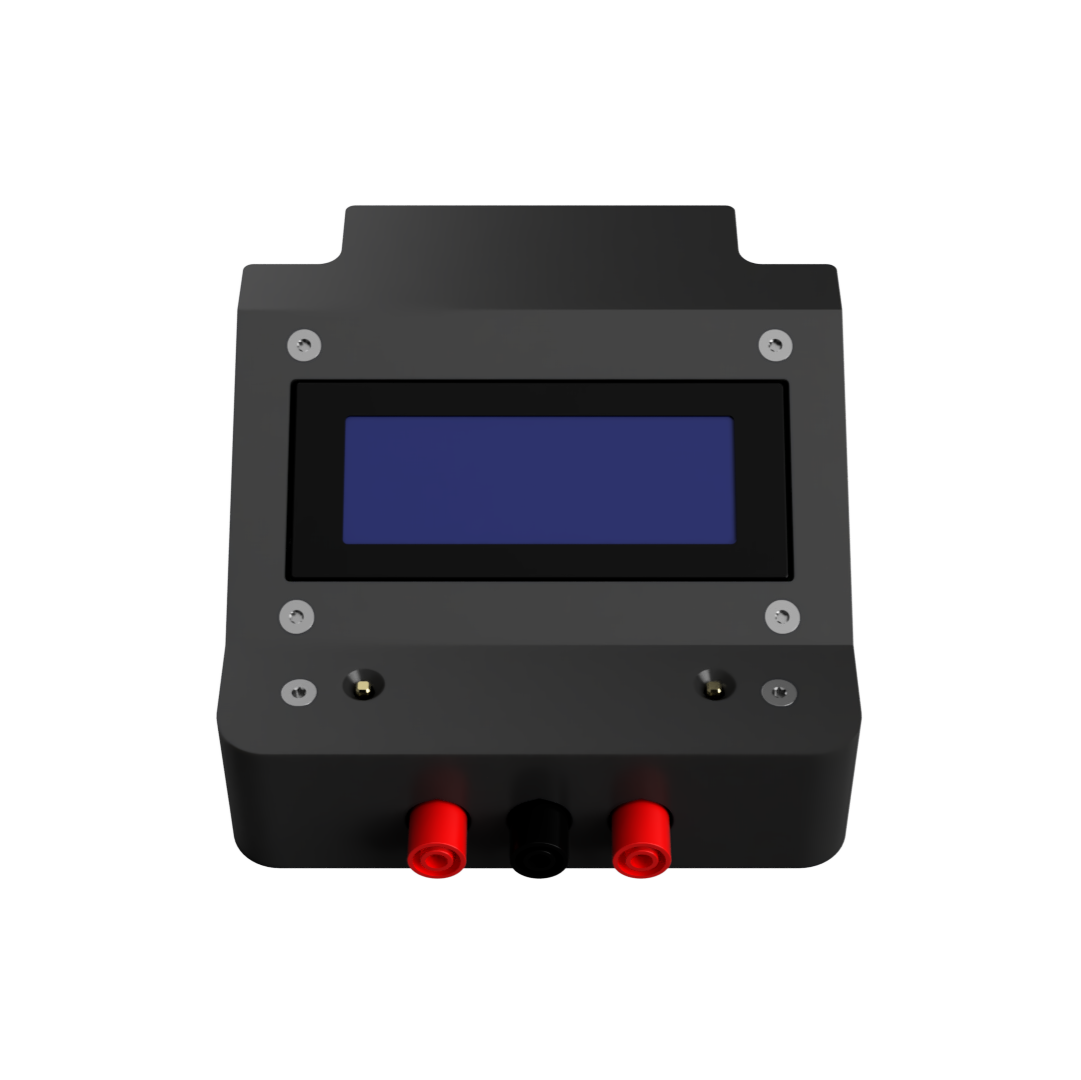
\includegraphics[width=0.95\textwidth]{images/SPROJ1_Rend.png}}

\pagestyle{fancy}
% \fancyhf{} % clear existing header/footer entries
% \renewcommand{\headrulewidth}{0pt}
% Place Page X of Y on the right-hand
% side of the footer
\fancyfoot[C]{Page \thepage \hspace{1pt} of \pageref{LastPage}}

\begin{document}

\maketitle

\label{sec:tableofcontents}
\tableofcontents
\section*{Contacts}
\vspace{1cm}
\begin{tabular}[h]{c}
     \textbf{Michał Sulej}   \\
     misul23@student.sdu.dk  \\
     \\
     \\
     \\
     \\
    \textbf{Theodor Erbs Dam Hansen}  \\
    thans22@student.sdu.dk            \\
\end{tabular}
\hfill
\begin{tabular}[h]{c}
     \textbf{Bence Tóth}    \\
     betot23@student.sdu.dk \\
     \\
     \\
     \\
     \\
     \textbf{Danial Jeddi}  \\
     dajed23@student.sdu.dk \\
\end{tabular}
\newpage

\section{Abstract}
\label{sec:abstract}
This report details the collaborative efforts of our group in designing and constructing a multimeter capable of measuring voltage, current, frequency, resistance, continuity, and temperature. Our work involved different aspects, like research, prototyping, circuit planning, coding, and addressing challenges that arose during the development process. In the end, we came up with a device that fulfills the requirements.
\section{Introduction}
\label{sec:introduction}

\subsection{Requirements}
This project aims to create a multimeter with the following requirements: 
\begin{itemize}
    \item Voltmeter with a range of 0 - 20V.
    \item Resistance meter.
    \item Two or more additional electrical quantities.
    \item Show measurements with correct units on the display.
    \item The final prototype should be a fully usable tool without any dangling wires and such.
    \item It should have a case and be portable.
    \item The user should be able to use a menu to select between functions.
    \item The main microcontroller should be protected so that it doesn't break during operation.
\end{itemize}

\subsection{Work Distribution}
The device is a result of the whole team working together. We decided to split the requirements into smaller, more manageable subsystems and assign a person to each one of them.
\renewcommand{\arraystretch}{1.3}
\begin{table}[h]
    \centering
    \begin{tabular}{|l|l|l|l|}
        \hline
        \textbf{Theodor} & \textbf{Bence} & \textbf{Michał} & \textbf{Danial} \\
        \hline
        Resistance Section & Frequency Section & Voltage Section & Temperature Section\\
        \hline
        Current Section & Firmware Development & PCB Design & \\
        \hline
        Mechanical Design & & Project Management & \\
        \hline
        % Bence & Frequency Section\\
        % Bence & Firmware Development\\
        % Theodor & Resistance Section\\
        % Theodor & Current Section\\
        % Theodor & Mechanical Design\\
        % Michał & Voltage Section\\
        % Michał & PCB Design\\
        % Danial & Temperature Section\\
    \end{tabular}
    \caption{Roles}
    \label{tab:roles}
\end{table}


\subsection{Terminations \& Acronyms}
\label{sec:terminations}
\renewcommand{\arraystretch}{1.5}
\begin{center}
\begin{tabular}{ | m{1.5cm} | m{5cm}| m{5cm} | } 
\hline
 \textbf{Term} & \textbf{Backronym} & \textbf{Meaning} \\ 
\hline
        PCB & Printed Circuit Board & A board with components and connections \\
        \hline
        V$_{\text{cc}}$ & Voltage collector, collector & The supply-voltage to the circuit \\
        \hline
        GND & Ground & The zero-potential plane of the circuit \\
        \hline
        ADC & Analog to digital converter & Converts analog signals to digital values \\
        \hline
        GPIO & General Purpose Input/Output & This describes the pins on the micro-controller \\
        \hline
        IC & Integrated Circuit & Semiconductor chip that performs specific functions \\
        \hline
        OP-AMP & Operational Amplifier & High-powered signal amplifier \\
        \hline
        LCD & Liquid Crystal Display & Screen with liquid crystals for displaying characters \\
        \hline
        MOSFET & Metal-Oxide-Semiconductor Field-Effect Transistor & Voltage controlled transistor \\
        \hline
        BJT & Bipolar-junction transistor & Current controlled transistor \\
        \hline
        MCU & Micro-controller Unit & IC used to execute the program \\
        \hline
        IRQ & Interrupt Request & Signal used to stop running a program in order to execute a special program \\
        \hline
        ISR & Interrupt Service Routine & A special function to execute during an interrupt \\
        \hline
\end{tabular}
\end{center}
\newpage
\section{Methods}
\label{sec:methods}
\subsection{Voltage measurement}
\label{sec:method_voltage}

\subsubsection{Idea}
Since we are using the internal ADC of the ATMEGA328P microcontroller, which has only a 10-bit ADC, we decided that it would be a good idea to try and make multiple ranges.
That is to make the most of the available resources.
We chose to make two ranges 0-5V and 5-20V. The range switch is performed automatically by the analog circuitry, not the MCU.

\subsubsection{Development}
During development, we faced many issues. Our initial attempts were made with TL072 OP-AMPs since they were in the university parts bin. However due to them not being a rail-to-rail variant, the output voltage couldn't go as low as we wanted it to go without a split rail power supply. 

After proper OP-AMPs arrived we got around to testing our design. After wiring the circuit it seemed to behave sporadically and not as intended. It appeared as if the OP-AMPs worked as an inverter when supplied with a 0V signal. Some forum posts suggested that it may be related to common mode rejection. However, later we found that the problem lied with the power supplies in the Mechatronics Lab. The output of the power supply began to oscillate with 2.5$V_{pp}$ after random amount time of operation. The solution is to just restart the power supply, either by turning it on and off or by turning the current limit to zero and back to some non-zero value. After testing the circuit with a working power supply the circuit worked flawlessly. 

Initially, the switching point was referenced with a zener diode. However, after assembling the first PCB, we found that the 4.8V zener supplied with 5V had a much lower voltage than expected thus we removed it and referenced the switching point to 5V. We could do that since the switching points' stability is not that important.

\subsubsection{Final Implementation}
In the beginning, the initial voltage is divided by four and buffered to not disturb it. The output of the buffer also creates a high range of the voltage measurement section. The schematic of which is shown in Figure \ref{fig:voltageSectionInput}.

\begin{figure}[h]
    \centering
    \frame{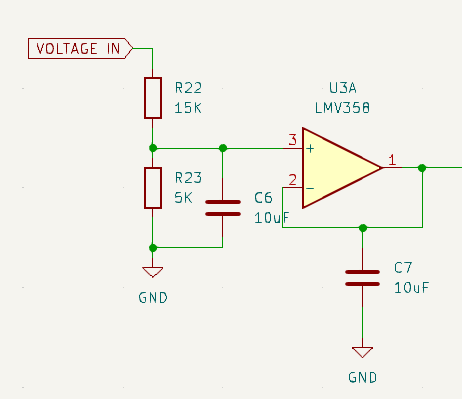
\includegraphics[width=0.5\linewidth]{images/voltageSectionInput.png}}
    \caption{The divider and buffer}
    \label{fig:voltageSectionInput}
\end{figure}

To get the lower voltage range, that is 0-5V, we applied a times four multiplier. That is to reverse the by-four division done by the voltage divider previously. Its schematic is presented in Figure \ref{fig:voltageSectionAmp}.

\begin{figure}[h]
    \centering
    \frame{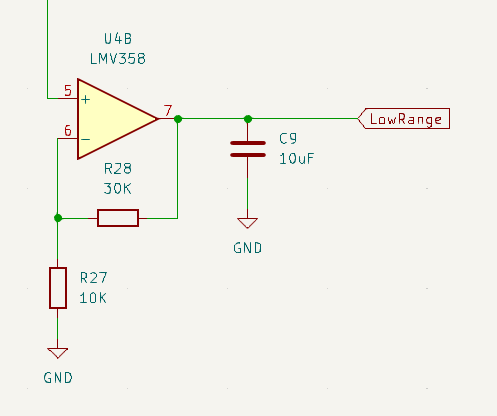
\includegraphics[width=0.5\linewidth]{images/voltageSectionAmp.png}}
    \caption{Lower range amplifier}
    \label{fig:voltageSectionAmp}
\end{figure}

Another part of the voltage section is the comparator which is responsible for detecting the point at which we switch between the different ranges. As we can see in Figure \ref{fig:voltageSectionComp} the comparator is made using the comparator configuration for an OP-AMP. The reference voltage doesn't have to be very stable since it just determines the switching point. The voltage at the inverting input is calculated using the following formula. $$V_{inv}=\frac{V_{ref}}{4}$$ The division is to compensate the initial division that scales the 0-20V to 0-5V.

\begin{figure}[h]
    \centering
    \frame{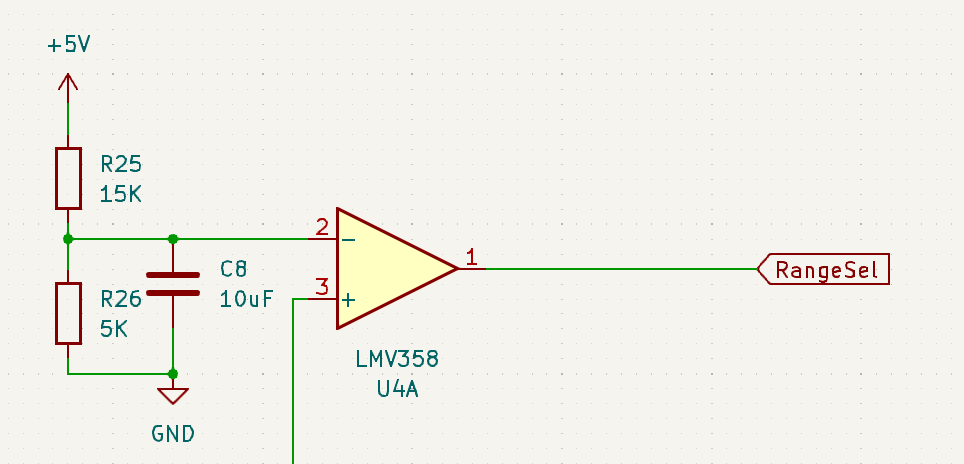
\includegraphics[width=0.5\linewidth]{images/voltageSectionComp.png}}
    \caption{Range select comparator}
    \label{fig:voltageSectionComp}
\end{figure}

The range switching itself is done by the use of a signal relay. To drive the relay we use a standard NMOS transistor. The circuitry can be seen in Figure \ref{fig:voltageSectionRelay}. The relay switches between the direct output of the buffer and the amplifier which are presented in Figure \ref{fig:voltageSectionInput} and Figure \ref{fig:voltageSectionAmp} respectively.

\begin{figure}[h]
    \centering
    \frame{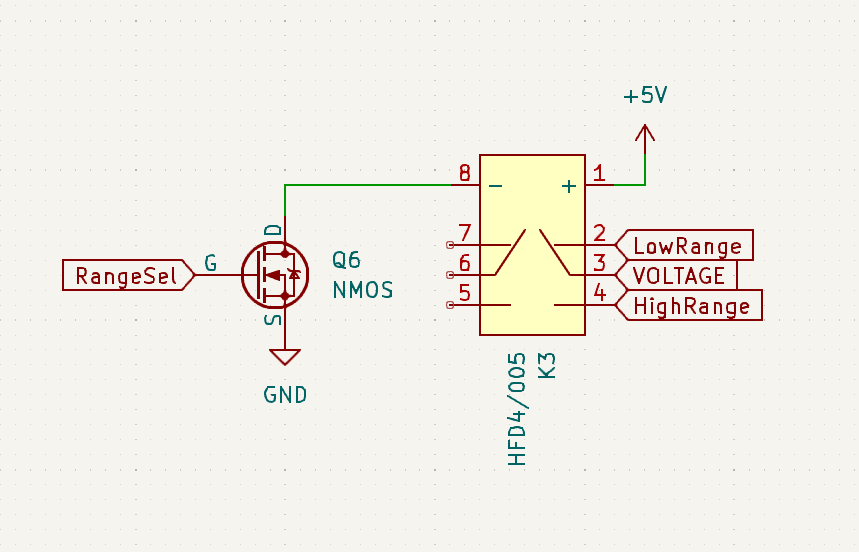
\includegraphics[width=0.5\linewidth]{images/voltageSectionRelay.png}}
    \caption{Range switching relay}
    \label{fig:voltageSectionRelay}
\end{figure}

The relay is controlled by the signal from the comparator. However, this signal also tells the microcontroller what range has been selected by the analog front end. The full circuit can be seen in the schematic, block 14. in section \ref{sec:appendix}.
\FloatBarrier
\subsection{Current measurement}
\label{sec:method_current}
This section shall describe the thought process and functionality of the current measurement part of the project.

\subsubsection{Idea}
As mentioned, we decided very early on that we wanted the current measurement as an extra feature for our product. The question then was, what methods were available to do this kind of measurement?
The two main categories of current measurement techniques we looked into were:
\begin{itemize}
    \item Voltage created over a known resistor
    \item Magnetic field created by current flowing through a coil
\end{itemize}

Before deciding, we first went on the easiest test, at least access-wise, which was voltage over a known resistor. This was done by designing a differential amplifier with an operational amplifier.
\begin{figure}[h]
    \centering
    \frame{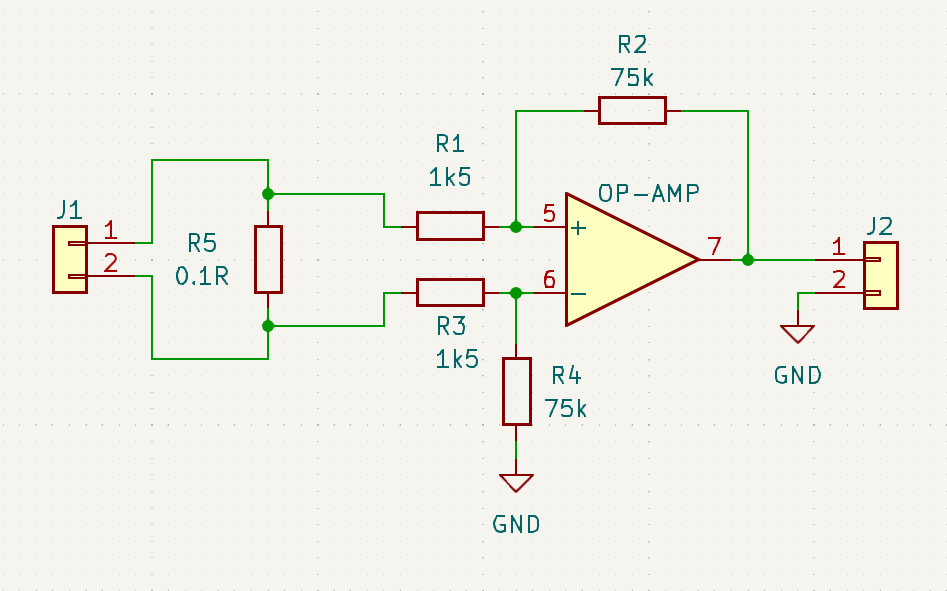
\includegraphics[width=\textwidth]{images/sch.diff.amp.png}}
    \caption{Differential amplifier used for testing}
    \label{fig:diff}
\end{figure}

As seen in Figure \ref{fig:diff}, the differential amplifier is built up by four resistors, the op-amp, and the shunt-resistor. This amplifier intends to magnify the voltage across the shunt-resistor, so the ADC in the Arduino can measure and then calculate the current flowing through the shunt, with the gain in mind.  The gain, in this case, was determined to be 50gg since our goal was a max current of 1A, and with a shunt resistance of 100m$\Omega$, this would result in an output of the amplifier to be 5V, which is the max input voltage. The gain was calculated with this equation, simplified:
\[V_{out}=(R_1/R_2)*(V_2-V_1)\]
Where the ratio between $R_1$ and $R_2$ is the overall gain and $V_2-V_1$ is the voltage difference that is multiplied.
\\
With this setup, we quickly discovered a limitation with this method, since there are special requirements for what is called a low-side measurement and a high-side measurement (Figure \ref{fig:hsls}). With the low-side measurement, this technique proved great, since this op-amp was an \textit{LM358APE4}, which has a very low common-mode voltage range that is ideal in this situation\footnote{See TI Application brief, References \ref{sec:references}}.

\begin{figure}[h]
    \centering
    \frame{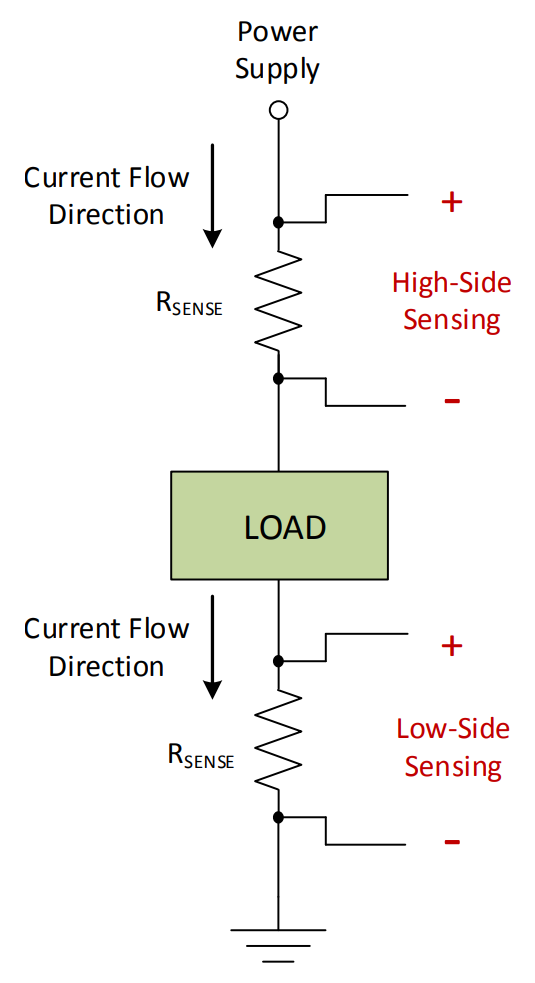
\includegraphics[scale=0.25]{images/hs_ls.png}}
    \caption{Specifying low-side versus high-side}
    \label{fig:hsls}
\end{figure}

But the opposite is the case with the high-side sensing, since in this instance the $V_{CM}$ is source dependent and thus can require a higher $V_{CM}$. This was where we decided on the other alternative to voltage over a known resistor. Because, with a multi-meter, you sometimes have to measure high-side and sometimes low-side, but the result can not be great if both considerations are implemented in the same design, since this would be paradoxical for an op-amp to have both properties.
\newpage
The current sensing method we then went with was the before-mentioned current through a coil. When this is the case, a magnetic field is created, and the magnitude of this field determines the current flowing through it. The limitations then are:
\begin{itemize}
    \item The thickness of the coil wire
    \item Saturation of the magnetic field
    \item Amount of winding
    \item Core material
\end{itemize}
And a way to measure the magnetic field.
With enough time to fine-tune these elements, this could be possible to implement ourselves, but we decided on buying an IC that would cover the whole spectrum with known elements.

\subsubsection{Implementation}
With the decision to go with an integrated circuit, the next step was to choose the sensor. With the limitation being the integrated ADC of the \textit{ATMEGA328}, we were looking for an analogue module, meaning the output voltage had to have a proportionality with the current. This voltage should have a high correlation with the current since we only have a 10-bit ADC.
\\ \\
We found a match on RS Components, mainly the \textit{ACS723LLCTR-05AB-T}. With the sensitivity being 400mV per 1A, this was the largest available. At the zero current, the output equates to $\frac{V_{CC}}{2}$, since this sensor is bidirectional in this case, 2.5V at 5V$_{CC}$. The \textit{ACS723} has a maximum current rating of 5A, at this current the max output voltage corresponds to 
\[V_{offset}+(V_{sens}*A)=V_{out}\Rightarrow2.5V+(0.400V*5)=4.5V\]
 The same is the case at -5A, hence 
\[2.5V+(0.400V*(-5))=0.5V\]
% \newpage
The magnetic field sensor used in this IC is a chopper-stabilized BiCMOS Hall IC. As illustrated by Figure \ref{fig:currentSens}\footnote{Illustration by Monolithpower, see References \ref{sec:references}} the conductor will generate a magnetic field, that is then picked up by the Hall transducer, and then amplified. 
\begin{figure}[h]
    \centering
    \frame{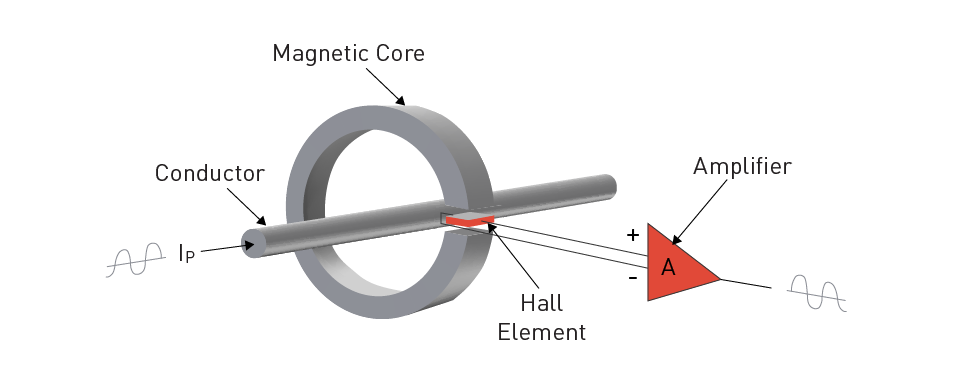
\includegraphics[width=\textwidth]{images/Current_Sensors_Article_Fig5-_960_x_385.png}}
    \caption{Current sens illustration}
    \label{fig:currentSens}
\end{figure}
\\
Another great feature of having this kind of sensor is the galvanic isolation between the two circuits, meaning the circuit measured cannot destroy or advisedly interfere with our system and vice versa. The only real interference when measuring a circuit would be the impedance introduced with IC, typically 0.65m$\Omega$ - basically nothing.

The \textit{ACS723} also has a tuned filter implemented that can be programmed by external components via its bandwidth select pin (6). If it is pulled down to GND, it selects the 80kHz range, while pulled up the filter is selected to be 20kHz. Since we can not utilize this extra bandwidth, and after some testing, we chose the 20kHz range by pulling it up to $V_{CC}$.
% \newpage
\begin{figure}[h]
    \centering
    \frame{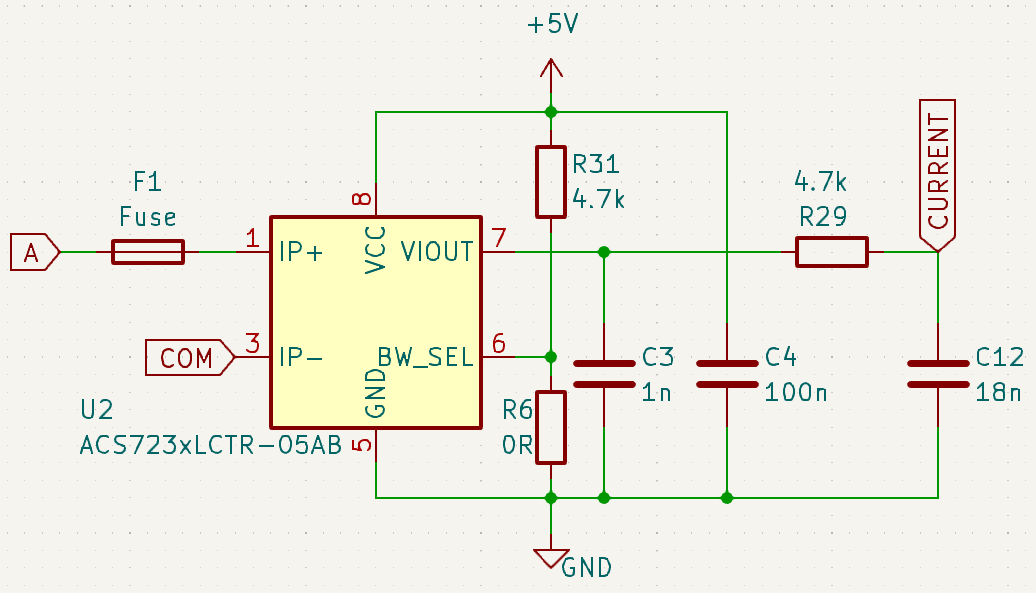
\includegraphics[width=\textwidth]{images/Current_sch.png}}
    \caption{Current sense schematic}
    \label{fig:CurrSch}
\end{figure}

For the circuit of the current sensor, see Figure \ref{fig:CurrSch}, we implemented a fuse of 5A and a low-pass filter. The filter is based on the sampling frequency of 20kHz mentioned before, to filter out unwanted noise. The dampening equates to -20dB since we used 2kHz as our cut-off frequency. With a predetermined resistor of 4.7k$\Omega$, we only need to determine the capacitor, in this case, C12
\[C_{12}=\frac{1}{2\pi*f_0*R}\Rightarrow\frac{1}{2\pi*2*10^3Hz*4.7*10^3\Omega}=16.9*10^{-9}F\Rightarrow18nF\]
With this 1$^{st}$-degree filter, the dampening equates to -20dB/decade, hence each doubling of frequency is a dampening of a factor of 10. Any higher frequencies picked up will be grounded by the capacitor.
\\\\
The fuse, F1, will be of a 5x20mm flick-type or F-type, meaning it will interrupt- or burn over quickly when it reaches 5A and not linger - thus fast-acting, to minimize the damage it might cause the IC. It is mounted on a PCB fuse block, thus making it easy to change.
% \newpage
\subsubsection{Code}
The code is set so the voltage we read from the \textit{ACS723} right when we switch to the function, via the buttons, is set as the voltage reference. This equates to about 2.5V but can vary quite a lot from time to time, $\pm$50mV, so it was necessary to measure the voltage at zero current draw, to the reference voltage. The voltage is sampled 100 times in the for-loop to remove unnecessary noise. With the known sensitivity of 400mV/A, and 10-bit ADC sampling, the current can be calculated, where \textit{value} is the filtered measured voltage from the loop:

\begin{align}
  & currFactor      &= &\hspace{2mm} \frac{1000}{400}                 &\text{(Sensitivity)} \notag \\
  & shuntVoltage    &= &\hspace{2mm} \frac{5}{1023}*1000*value       &\text{(ADC 10-bit value to voltage)} \notag \\
  & current         &= &\hspace{2mm} (shuntVoltage-V_{ref})*currFactor   &\text{(Actual current)} \notag \\
  \notag
\end{align}

\subsection{Frequency measurement}
\label{sec:method_frequency}

\subsubsection{Idea}
From the beginning, we thought about measuring not only square-wave signals, but triangle, saw-tooth, and any other type of signal, as long as they have a single dominant frequency. For this reason, we opted to use a \textit{SN74HC14} Schmitt-trigger inverter to convert any type of signal to a square wave, which can be directly read by the GPIO pin of the Arduino microcontroller. Using a 5V Zener diode as a clamping diode for the input of the Schmitt-trigger. To further improve the capabilities of our frequency front-end, we used a capacitor to AC couple the input, thus removing its DC offset. Next we set our own offset right at the switching point of the Schmitt-trigger. By doing this we decreased the minimum amplitude that the input signal has to have. When it comes to the frequency measurement capabilities we found that the lower limit of this method seems to be around 25Hz, while the upper limit is around 100 kHz, with a maximum allowed error of $\pm$5\% taken into consideration.
The schematic for the frequency measurement can be seen in section \ref{sec:appendix}. See the full schematic, in block 9.

\subsubsection{Code implementation}
The method for measuring frequency is based on the built-in Arduino function called \textit{pulseIn}. This function returns the amount of time it took (in microseconds) for the voltage at the specified input pin to go from either HIGH to LOW or from LOW to HIGH level. By measuring both scenarios we get the whole period of the signal. We can calculate the frequency by taking the reciprocal of the sum of these two timeouts given by the \textit{pulseIn} function.
\subsection{Resistance measurement}

\subsubsection{Idea}
\label{sec:method_resistance_idea}
With the overall feature idea being auto-range, the resistance measurement is no exception. We knew we needed more than one voltage divider, meaning more than one voltage divider with a known resistance of R1. See Figure \ref{fig:vol_div}. This means there needed to be a solution to be able to switch between these known resistors since the optimal configuration is to have the highest V$_{\text{CC}}$ possible, for better accuracy. This can be done by either removing the V$_{\text{CC}}$ for the resistors not being used, or removing the ground plane.
In this case, we opted for removing V$_{\text{CC}}$, since we wanted to do this with transistors. We chose MOSFET specifically, since they have a very low impedance when saturated, compared to the average BJT. And since the voltage across the unknown resistor can vary between 0V to 5V, thus the Source-pin, the N-channel variation is not optimal, whereas the P-channel is well suited since the Source-pin is always the same. Hence, we opted for five different values, since that can cover a large enough resistance spectrum for our purpose. This also implies that we need five GPIO-pins, other than the analogue-pin, which we only have a limited supply of. But it is needed. For the schematic used, see section \ref{sec:appendix}, the full schematic, block 8. We opted for the P-channel MOSFET \textit{IRLML6401TRPBF}, since it proved to have a saturation impedance, R$_{\text{DS(ON)}}$, of only 0.05$\Omega$, limiting the parasitic resistance in our measurement of the known- and unknown resistor.

\begin{figure}[h]
    \centering
    \frame{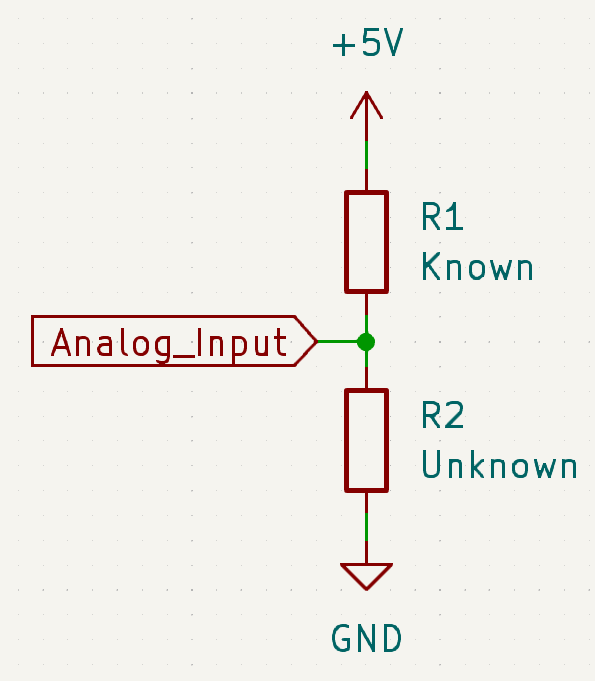
\includegraphics[scale=0.25]{images/Vol_div.png}}
    \caption{Voltage Divider setup}
    \label{fig:vol_div}
\end{figure}

\subsubsection{Code implementation}
\label{sec:method_resistance_code}
The data sampling and evaluation are done using two nested for-loops and a switch statement. The first loop iterates through as many times as it is declared beforehand using a constant. This loop is used for averaging out the final value. The second, inner for-loop does the data collection. The data is stored in an array, whose elements correspond to the measured values at the different resistance ranges. Using the function called \textit{setResistancePin}, the 5 control pins of the PMOS transistors are switched so that only one is active at any given time (the selected pin will be LOW, while the other pins HIGH). After the correct range has been selected using this method, the value measured by the ADC of the MCU is stored at the particular index of the array. There is a small delay of approximately 4 milliseconds between the measurements to let the voltage settle at the input pin. To get the range that is closest to 2.5V (half of the V$_{CC}$), the function \textit{getClosestToHalf} is used. This function iterates through the array of measured values and updates the correct index to be used by checking the size of the difference between the measured value and 512 (i.e. half of the maximum resolution of the built-in ADC, 10 bits - 1023 is the maximum value). After the correct index to be used is found, the values for the variables used in the final calculation are chosen in a switch statement. The value of the unknown resistance is found by the following formula:
\vspace{1cm}\[R_X=\frac{M*R_N}{2^A-1-M}\]
where: \[R_X , R_N , M , A\] are the unknown resistance value, known resistance value (selected range), the measured digital value and the resolution of the ADC, respectively. After the loops have finished, the result is averaged out. Before displaying the final value, a function called \textit{checkDisconnectedRes} is used to check whether there is an actual resistor connected to the input terminals or not. This function iterates through the array of measured values, checking whether the values are below a certain threshold value. If all the values at the specific ranges are below this threshold value, that means that there is nothing connected to the input terminals, thus nothing is displayed. Otherwise, the calculated resistance value and the selected range are displayed on the LCD screen. With this method, we can measure resistances from 0 $\Omega$ up to around 3 M$\Omega$ with adequate precision.


\subsection{Temperature measurement}
\label{sec:method_temperature}
This section shall describe the thought process and functionality of the temperature measurement part of the project.

\subsubsection{Idea}
The first idea for this challenge was to implement a temperature-dependent resistor with a positive temperature coefficient, PTC. This is a resistor whose resistance value will increase when the temperature does. The corresponding voltage across the resistor will change as well, thus making it possible to measure the temperature that way, since we know what its value is at a certain temperature, it can be calculated from said voltage.
Another solution would be a dedicated IC that has built-in stabilization and better-known and documented properties. This would also speed up calibration time and decrease implementation difficulties.

\subsubsection{Implementation}
We settled with the idea of an IC, just to speed up the research and development. The IC of choice landed on the \textit{LM35}, which has an analogue output that corresponds to its current temperature. Time was running short, so we included it in a very basic form, to be expanded in some future feature work-over. The code we ended up writing was heavily inspired by the LM35 library seen in section \ref{sec:references}.
\subsection{Continuity test}
\label{sec:method_continuity}

\subsubsection{Idea}
Most digital multimeters on the market come with an option to measure the continuity of the circuit, i.e. whether the measured trace is intact or not. This type of measurement comes in handy while troubleshooting a PCB, as there could be traces that are damaged, hence not making a proper contact, causing the circuit to not function as it is intended. For this measurement the resistance circuit is used, which has been previously discussed. 

\subsubsection{Code implementation}
The continuity test uses the same method as the resistance measurement, but here the selected range is fixed to be the one containing the 100$\Omega$ resistor. After the value of the resistance is calculated using the aforementioned formula, this value is compared to the maximum allowed value of 10$\Omega$. If the calculated value is below this threshold, the piezoelectric buzzer is activated using the built-in Arduino function \textit{tone}, which produces a square wave signal at a chosen frequency of 1kHz. In this case, the value of the resistance is displayed on the LCD screen as well.
\newpage
\subsection{Mechanical design}
\label{sec:method_mechanical}
This section shall describe the thought process and functionality of the mechanical part of the project.

\subsubsection{Idea}
The main constriction, the bulky 4x20 LCD, limits the compactness of the design. On the other hand, it simplifies the final product because there are limited options to include the display logically.

Right from the get-go, we decided that the switching between modes would not be done via a rotary switch, but rather digitally via a relay-matrix. This is important for mechanical design since it determines the functionality and what is needed to consider when designing the enclosure. By using the digitalized version of switching between modes, the only things we needed access to from the outside of the enclosure were:
% \newpage
\begin{itemize}
    \item Two buttons to control the modes (Next mode - previous mode)
    \item Reading the LCD
    \item Easy access to the 9V battery
    \item Being able to access the on/off switch
    \item Program the Arduino Nano
    \item Access to screws to disassemble the multi-meter
\end{itemize}
And with the exterior brainstormed, the interior needed some thinking. The requirements there would be:
\begin{itemize}
    \item An isolated place for the battery
    \item A way to fasten our PCB
    \item Somehow be able to access the buttons from the PCB
    \item The assembly screws to have threads to attach themselves
\end{itemize}
\label{sec:points}
\newpage
\subsubsection{Implementation}
With the points in \ref{sec:points} as a guide, the design would centre around the LCD. We decided that the best way to see the display from as many angles as possible, the LCD would need to be angled, in this case 30$^{\circ}$. \newline
The PCB will be mounted on the bottom of the case and the inner surface area will determine the cut-out of the PCB. This was done with the CAD-program Fusion 360 from Autodesk, a sketch-based CAD entity. This allows us to export the sketch we created, determining the dimensions of the PCB, to an .dxt-file which can be imported to KiCad 7.0, as a cut-out. By doing it like this, we can also direct where the mounting holes will be so that they will line up.
The sketch also considers the placement of both the 9V battery as well as the ON/OFF switch. This can be seen in Figure \ref{fig:sketchPCB}.
\begin{figure}[h]
    \centering
    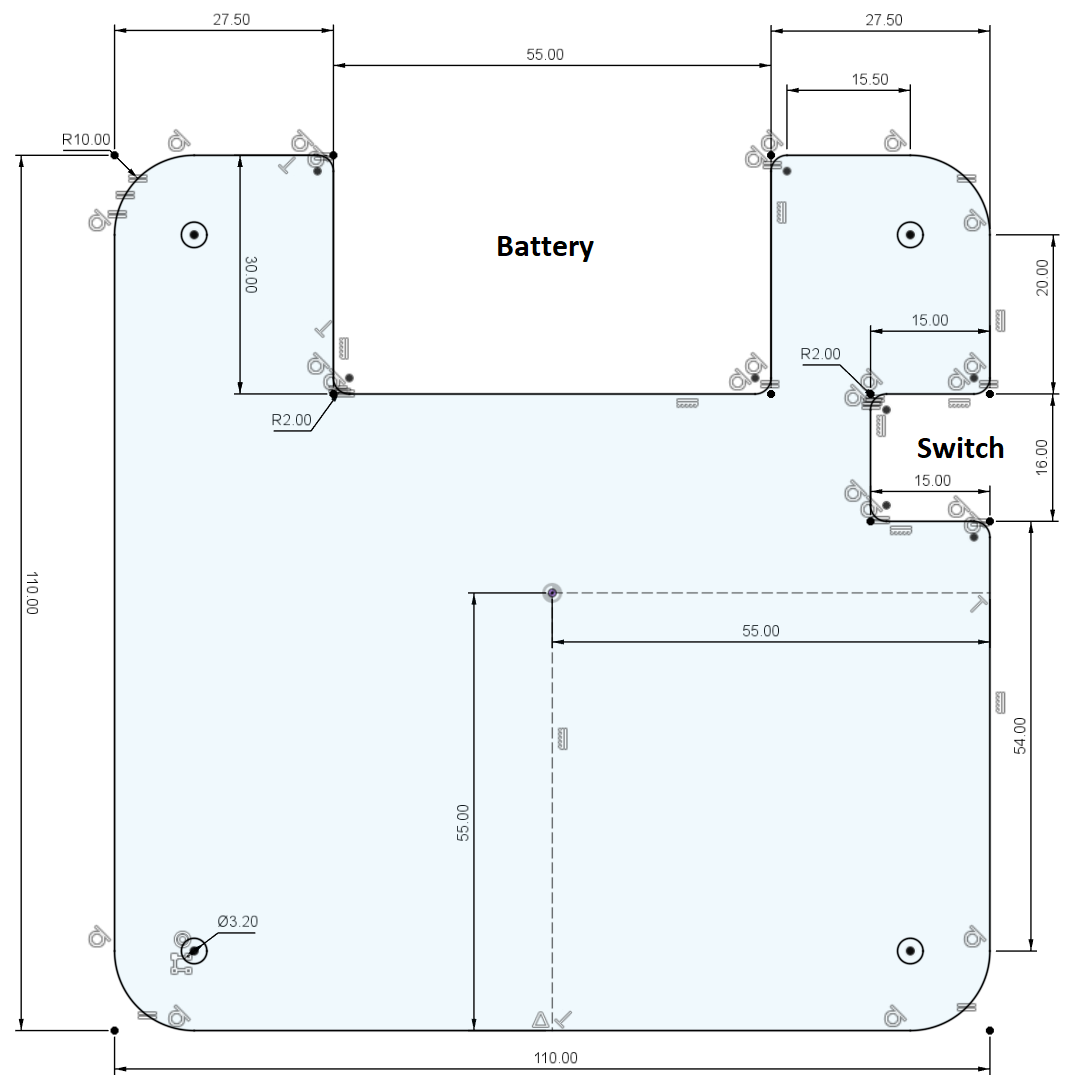
\includegraphics[width=\linewidth]{images/sketch-pcb-cutout.png}
    \caption{Final sketch of the PCB cut-out}
    \label{fig:sketchPCB}
\end{figure}
\newpage 
\noindent By importing various components to Fusion 360, it was also possible to place these components on the extruded PCB, to then help visualize how the next steps of the design process should proceed. Things like:
\begin{itemize}
    \item Placement of the two buttons needed for the menu switching
    \item Where the three 4mm banana plugs will stick out
    \item Placement of the Arduino Nano port
\end{itemize}
\begin{figure}[h]
    \centering
    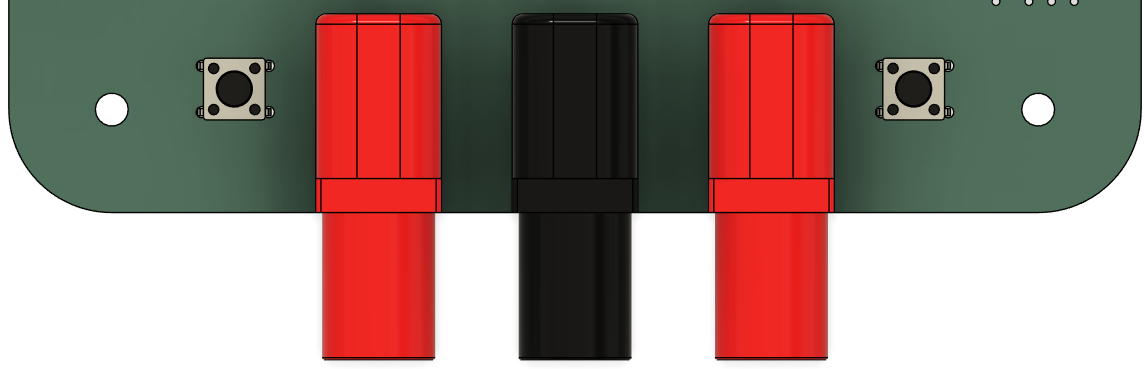
\includegraphics[width=\linewidth]{images/sketch-placement-plugsbut.png}
    \caption{Example of the placement of plugs and buttons}
    \label{fig:placeplugbut}
\end{figure}
Figure \ref{fig:placeplugbut} shows that the placement can easily be visualized. By then using measurements, the positioning of these components can be translated into the layout section of the PCB design in KiCad.
This comes with a trade-off, because the PCB is at the bottom of the case, the buttons would not be reachable. This problem is solved with what is called a 'button guide'. This was made with a 3D-printed cylinder which makes the buttons reachable from the outside.

This is shown in Figure \ref{fig:guide}.
\begin{figure}[h]
    \centering
    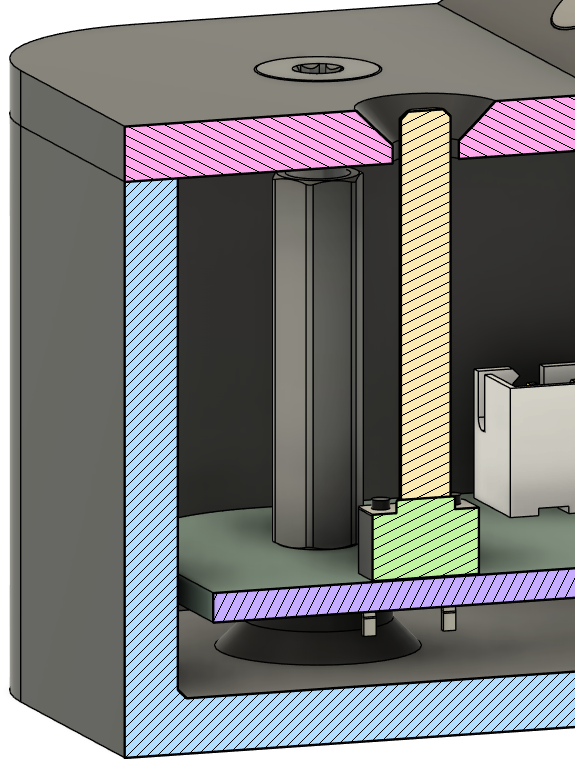
\includegraphics[width=0.35\linewidth]{images/guide.png}
    \caption{'Guide'-concept (\textcolor{GreenYellow}{yellow}), button (\textcolor{green}{green})}
    \label{fig:guide}
\end{figure}
\newpage
The mounting of the PCB to the bottom case was done via four extruded cylinders, where there was room enough to include M3 brass threaded inserts. These are inserted after the case is printed, with the tool soldering iron, set at 160$^\circ$-Celsius. This is illustrated in Figure \ref{fig:thread1}
\begin{figure}[h]
    \centering
    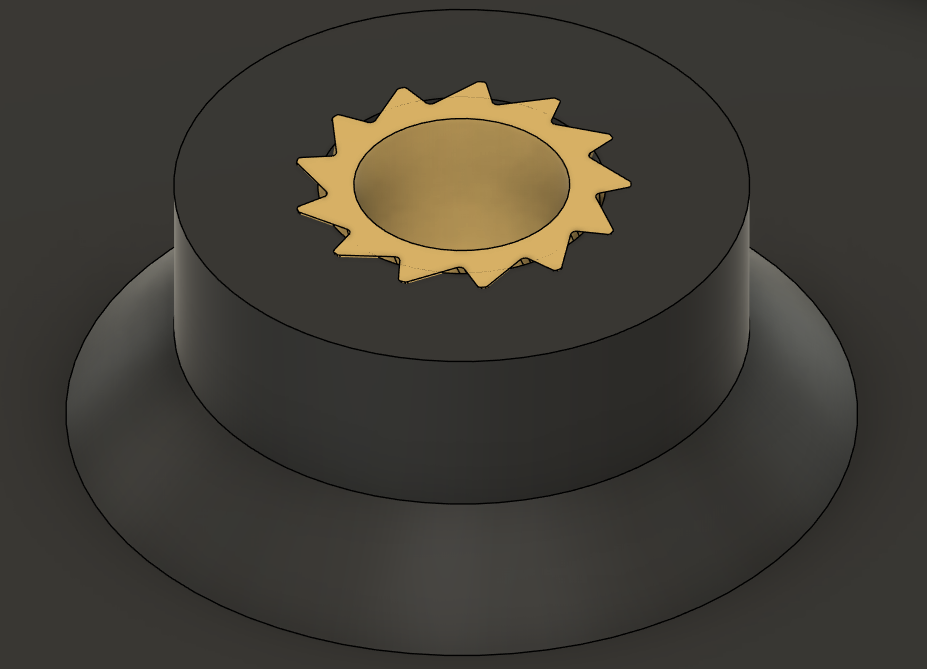
\includegraphics[width=0.5\linewidth]{images/threadinsert.png}
    \caption{Extruded cylinder w. threaded insert}
    \label{fig:thread1}
\end{figure}

We chose to have a no-tool hatch for easy access to the battery. With the combination of the 'battery low notification' via the LCD, it is then trouble-free to change the battery out in the field. This is seen in Figure \ref{fig:lid}.
\begin{figure}[h]
  \centering
  \subfloat[Without lid]{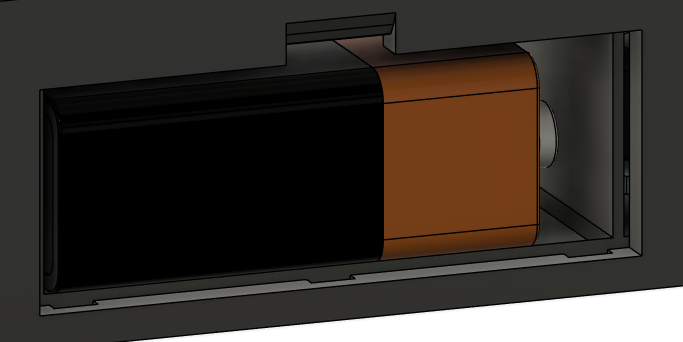
\includegraphics[width=0.4\textwidth]{images/batwolid.png}
  \label{fig:lida}}
  \hfill
  \subfloat[With lid]{
\includegraphics[width=0.375\textwidth]{images/batwlid.png}
  \label{fig:lidb}}
  \caption{Battery-lid placement}
  \label{fig:lid}
\end{figure}

To help isolate the battery, the bottom part of the case comes with a built-in 1mm wall separating the battery and the PCB. This is done for safety concerns since the possibility of short-circuiting is present. This is shown in Figure \ref{fig:batiso}.
\begin{figure}[h]
    \centering
    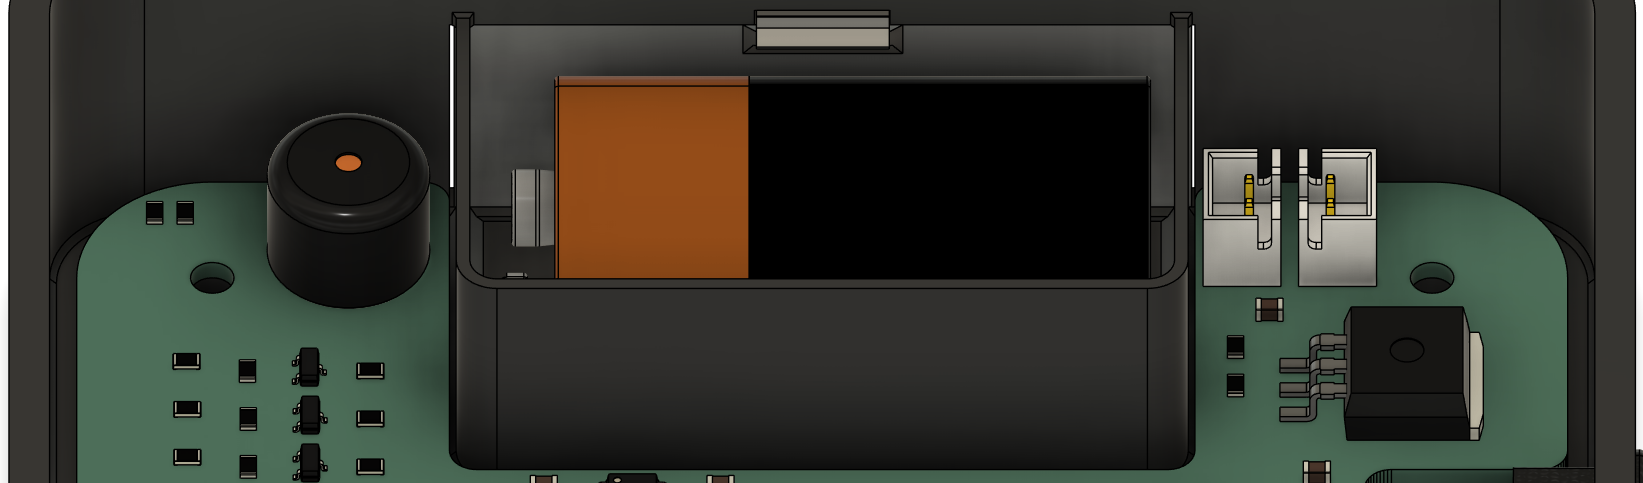
\includegraphics[width=0.855\linewidth]{images/batiso.png}
    \caption{Wall between PCB and battery}
    \label{fig:batiso}
\end{figure}
\newpage 
\noindent 
To then attach the upper part of the case, the lid w. the LCD, the method was to combine our threaded inserts and then attach PCB spacers at a length of 20mm. This is seen in Figure \ref{fig:guide} as the grey column with the screw attached.

\begin{figure}[h]
  \centering
  \subfloat[Without top]{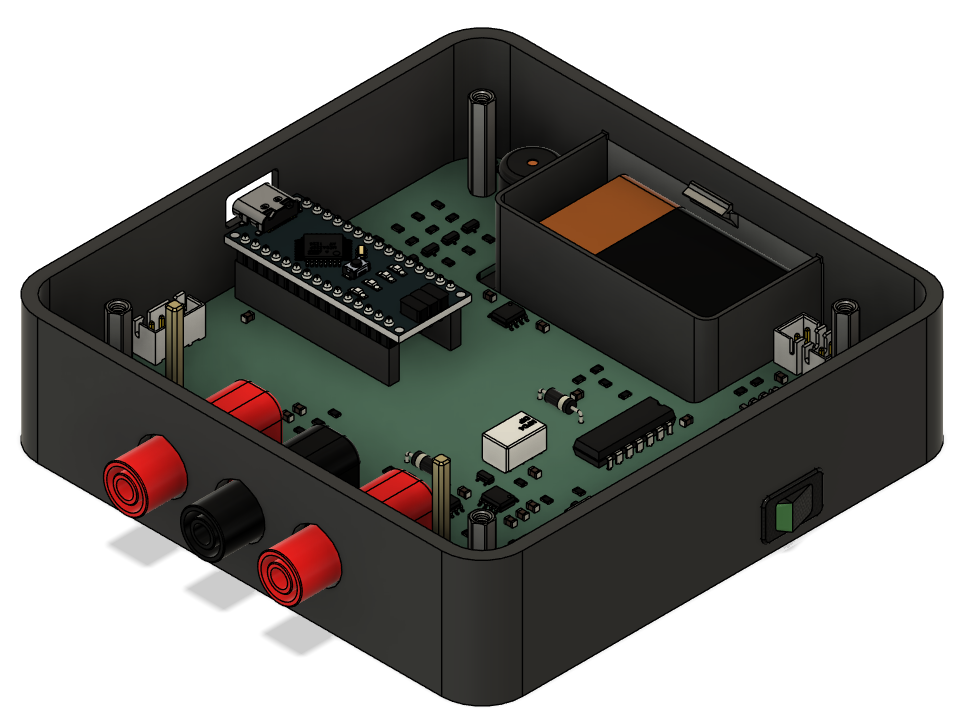
\includegraphics[width=0.65\textwidth]{images/bottom.png}
  \label{fig:enclA}}
  \hfill
  \subfloat[With top]{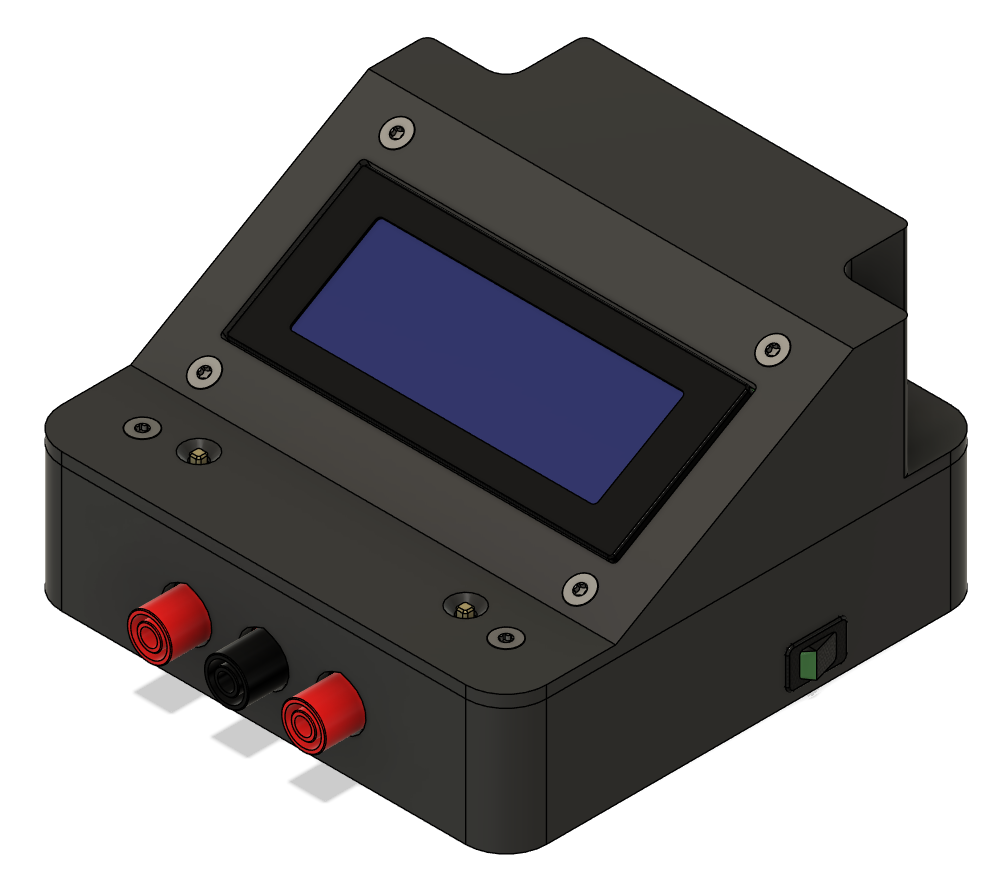
\includegraphics[width=0.65\textwidth]{images/total.png}
  \label{fig:enclB}}
  \caption{Final product}
  \label{fig:lid}
\end{figure}

\noindent The enclosure material is PLA+ and printed using a private Prusa MK3S+ FDM printer. See the Appendix for the top and bottom drawings of the enclosure.
\newpage
\subsection{Miscellaneous}
The whole project code and the PCB design can be accessed via the corresponding links in section \ref{sec:references}.

\subsubsection{Switching between measurement modes (code description)}
\label{sec:method_switch_code}
At the beginning of our project, we thought of a couple of switching methods. One of our ideas was to use multiple buttons, one for each measurement type. This method would make up for a simpler code implementation but would require a tremendous amount of pins on the MCU. Due to this drawback, we opted out of this method. Another method we discussed was the use of a rotary encoder, but in the end, we opted to use just two buttons, as a means of switching through the measurement modes in a menu-like way. The buttons are used to switch to the previous or the next measurement type, respectively. This way, we only use two pins, and could easily extend the types of measurement, without changing the front end of the code. The two buttons are connected between two IRQ pins of the MCU and ground. The internal pull-up resistors of the two pins are activated in code, this way there is never an unknown state at the used pins, which could trigger a false switch. The whole switching methodology relies on the use of interrupts, rather than the often-used polling method. The two ISRs, which are being called at a triggered interrupt, are one-line functions, flipping either the "next" or "prev" boolean variables to true. Using the Arduino framework's \textit{attachInterrupt} function, these ISRs are attached to their matching IRQ pins, specified to trigger an interrupt only at a falling edge, i.e. when the logic level at the input goes from HIGH to LOW. In the main loop, these two variables are checked whether they are true, in which case another variable, "mode select", is incremented or decremented. At every interrupt detection, a delay of approximately 170 milliseconds is used to counter the buttons' rapid on-off clicking, which is due to mechanical contact and imperfections in the buttons' construction. Based on the "mode select" variable, the specific measurement mode functions are then selected in a switch statement. During this time, the specific relay combination is selected as well, within the function called \textit{selectRelayCombination}, based on section \ref{sec:method_safety_relays}.

\subsubsection{Battery level indicator}
\label{sec:method_bat_indicator}
The ability to alert the user to change the battery is a crucial one, especially in a device like a multimeter. For this reason, we wanted to include some sort of alerting system in our device, too. As the MCU is powered through an LM7805 linear voltage regulator IC, so we chose the minimum adequate voltage level based on its datasheet. The datasheet states that the minimum input voltage required to maintain line regulation is 7.5V, so we chose this value as well. The voltage of the battery is read using an ADC pin and a voltage-divider of two identical, 100k$\Omega$ resistors. As the voltage-divider in this configuration will always output half of the supply voltage (in our case the voltage level of the battery), the specified minimum voltage level used in the code is also halved, i.e. 3.75V. At every measurement mode switching, a battery voltage level test takes place. If the supply voltage is below the specified threshold, an alerting message will appear on the fourth line of the LCD. This alert will not render the device unusable, it is there just to alert the user, as intended.

\subsubsection{Safety and mode switching}
\label{sec:method_safety_relays}
Our multimeter comes with safety measures for each of our modes. These are:
\begin{itemize}
    \item Voltage:      Built-in protection diodes in the buffer op-amp. (Up to 5mA)
    \item Current:      A 5A fuse and temperature shut-off built-in
    \item Resistance:   Diode to prevent outside voltage from interacting with the analogue pin
    \item Frequency:    Capacitor to interrupt DC-voltage and a zener-diode to prevent a voltage over 5V
\end{itemize}

\begin{figure}[h]
    \centering
    \frame{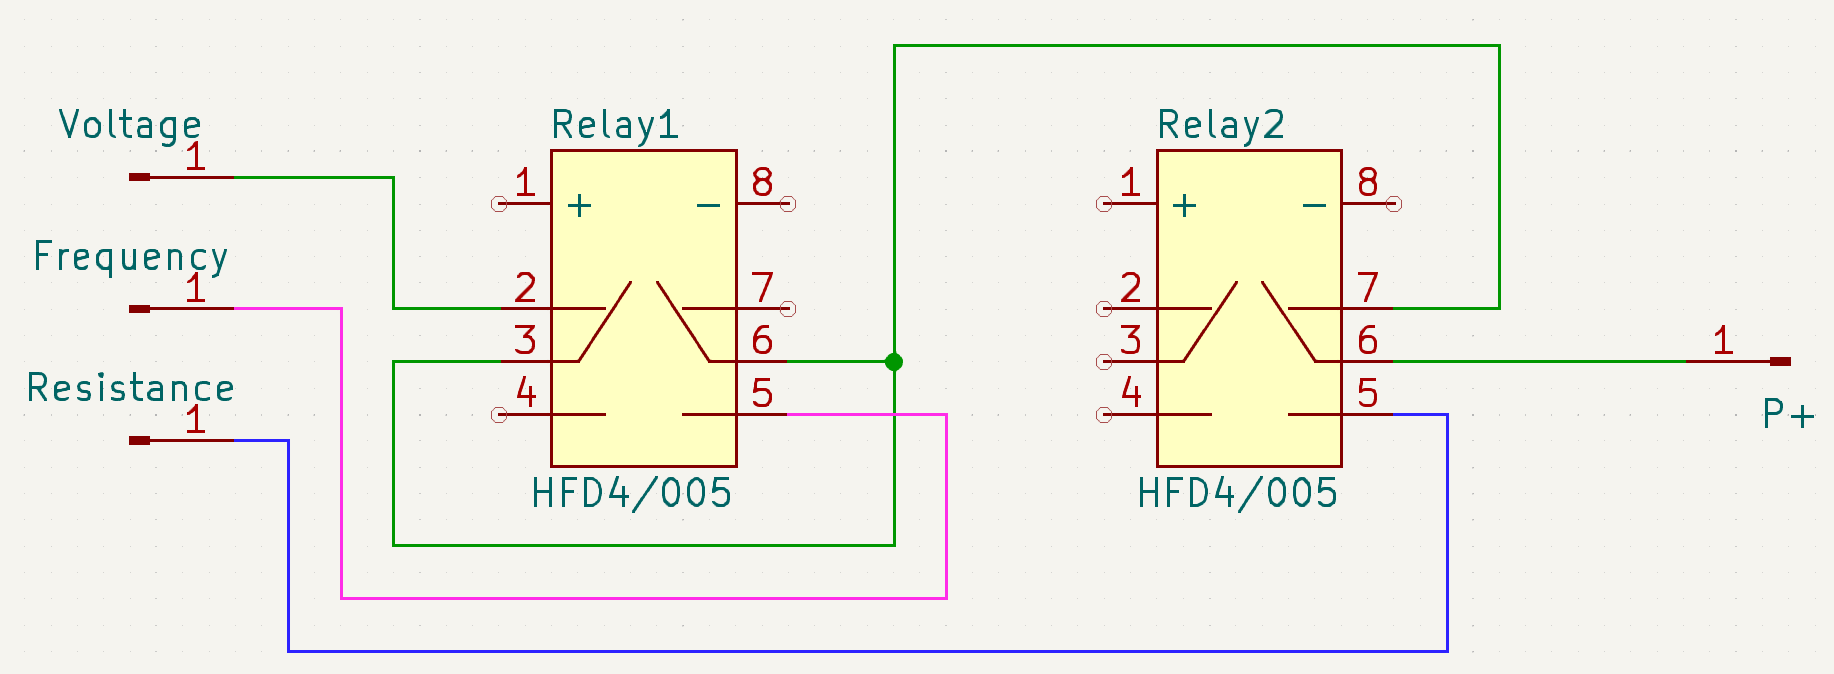
\includegraphics[width=1\linewidth]{images/RelayMat.png}}
    \caption{Relay-matrix principle}
    \label{fig:relmat}
\end{figure}

\noindent The method we used to switch between our modes was via two signal relays. This principle is shown in Figure \ref{fig:relmat} and the logic is:

\begin{itemize}
    \item Voltmeter mode: Relay1 \textcolor{red}{OFF} / Relay2 \textcolor{red}{OFF}
    \item Ohmmeter mode:  Relay1 \textcolor{red}{OFF} / Relay2 \textcolor{green}{ON}
    \item Frequency meter mode: Relay1 \textcolor{green}{ON} / Relay2 \textcolor{red}{OFF}
\end{itemize}

\noindent This makes sure that only one mode is connected to the probe input at a time, while the other ones are galvanic disconnected. The drawback then is the current draw derived from keeping the relays in the ON-state when using the ohmmeter and frequency meter.

\subsubsection{Project management}
Project management mainly involved creating the time plan which can be seen in the Appendix, distributing tasks to team members, setting up project infrastructure, and keeping the project on track. All of the decisions made were made with the consent of the majority of the team members. See Figure \ref{fig:TP} for a detailed plan of our project.

\subsubsection{Economy}
The whole project cost 1036.7 DKK. The bill of materials can be seen in section \ref{sec:appendix}, Appendix.
\newpage
\section{Results}
\label{sec:results}
\subsection{Voltage}
\label{sec:results_voltage}

These are our results when measuring voltage with our multimeter. The tests were performed with a power supply sweeping the voltage from 0 to 20V. While this was happening the voltage was measured by our multimeter and a calibrated one. The test has been performed with the use of Keysight 34461A Digital Multimeters which is referred to as Calibrated.

\begin{figure}[h]
    \centering

    \begin{tikzpicture}

    \begin{axis}[legend style={at={(0.95, 0.1)},anchor=south east}, width=\linewidth, height=5cm,
        title = {Voltage Measurement},
        xlabel = {Target [V]},
        ylabel = {Measured [V]}]
        \addplot[blue, mark=*] table {Results/VoltData/VoltageMeasCal.dat};
        \addlegendentry{Calibrated}
        \addplot[red, mark=*] table {Results/VoltData/VoltageMeasOur.dat};
        \addlegendentry{Voltmeter}
    \end{axis}

    \end{tikzpicture}

    \caption{The measured voltage by both calibrated and our multimeters from what target was set.}
    \label{fig:ResVoltageMeas}
    
\end{figure}
% \begin{figure}[h]
%     \centering
%     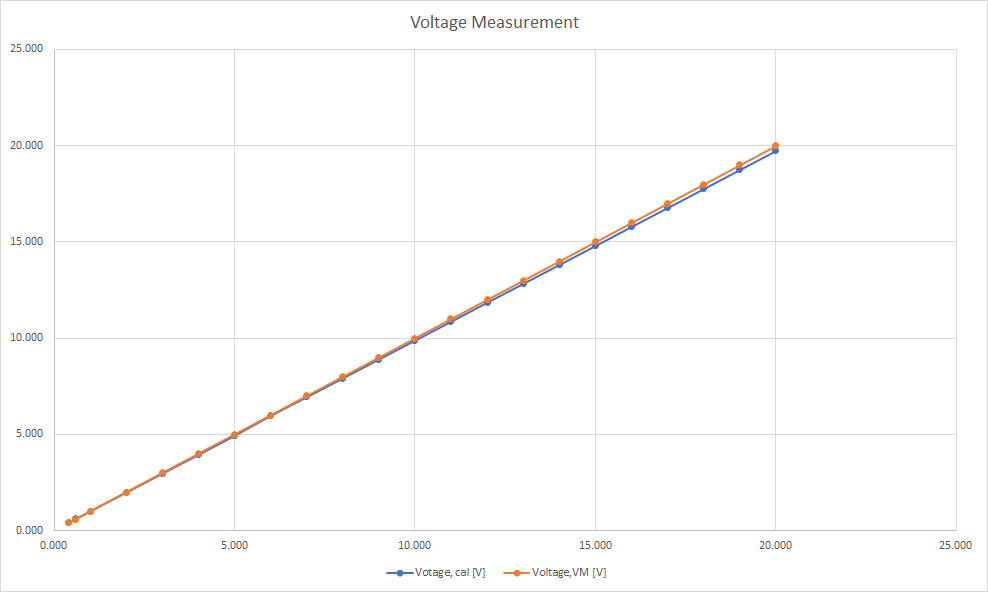
\includegraphics[width=0.80\linewidth]{images/voltageMeas.png}
%     \caption{Voltage Measurements}
%     \label{fig:ResVoltageMeas}
% \end{figure}
Figure \ref{fig:ResVoltageMeas} shows the voltage measured by a power supply internal meter, the calibrated one as well as ours.

\begin{figure}[h]
    \centering

    \begin{tikzpicture}

    \begin{axis}[legend style={at={(0.95, 0.4)},anchor=south east}, width=\linewidth, height=5cm,
        title = {Percentage deviation, voltage},
        xlabel = {Target [V]},
        ylabel = {Percentage [\%]}]
        \addplot[red, mark=*] table {Results/VoltData/VoltageDeltaCal.dat};
    \end{axis}

    \end{tikzpicture}

    \caption{The difference from the target or the measured value by the calibrated multimeter at different target settings.}
    \label{fig:ResVoltageDelta}
    
\end{figure}
% \begin{figure}[h]
%     \centering
%     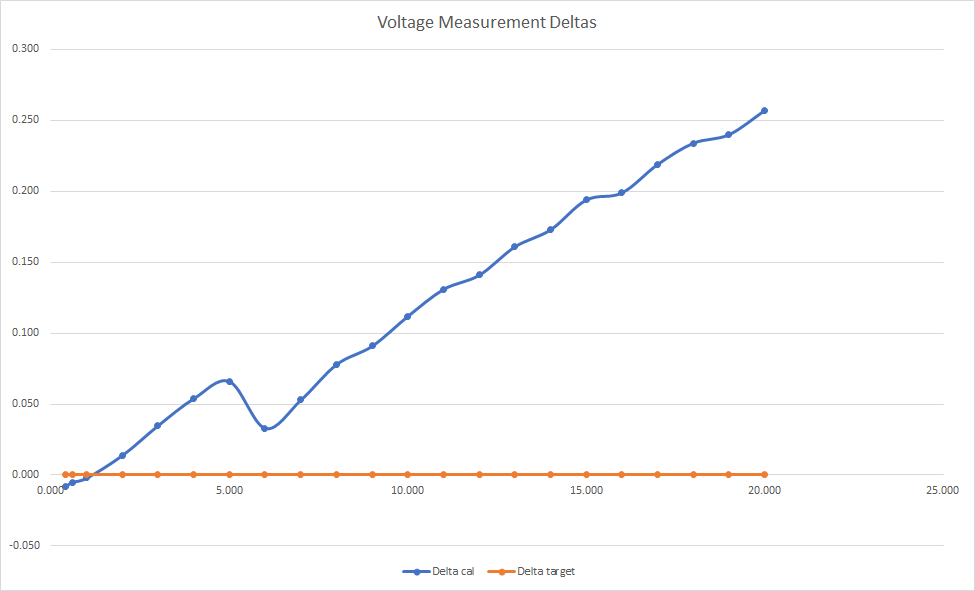
\includegraphics[width=0.80\linewidth]{images/voltageDelta.png}
%     \caption{Voltage Deltas}
%     \label{fig:ResVoltageDelta}
% \end{figure}
Figure \ref{fig:ResVoltageDelta} shows the difference between our multimeter measurement and the measurement of the calibrated one as well as the set point on the power supply. See Figure \ref{fig:VM1} for test setup.

\subsection{Frequency}
\label{sec:results_frequency}
These are our results for the frequency measurement. Although multiple signal wave forms were tested, the signal in the displayed data was a sine-wave, supplied by a Tektronix AFG1022 function generator. The frequency displayed by our multimeter was compared to the value displayed by a Tektronix MSO 2014 Mixed Signal Oscilloscope calibrated in 2023 by Trescal.

\begin{figure}[h]
    \centering
    \begin{tikzpicture}
    \begin{axis}[legend style={at={(0.95, 0.09)},anchor=south east}, width=\linewidth, height=6cm,
        title = {Frequency Measurement},
        xlabel = {Target [Hz]},
        ylabel = {Measured [Hz]}]
        \addplot[blue, mark=*] table {Results/FreqData/freqDataCal.dat};
        \addlegendentry{Calibrated}
        \addplot[red, mark=*] table {Results/FreqData/freqDataFM.dat};
        \addlegendentry{Freqmeter}
    \end{axis}
    \end{tikzpicture}
    \caption{Comparing the results between our frequency meter and the calibrated oscilloscope}
    \label{fig:freqGraph}
    
\end{figure}

\begin{figure}[h]
    \centering
    \begin{tikzpicture}
    \begin{axis}[legend style={at={(0.95, 0.8)},anchor=south east}, width=\linewidth, height=4cm,
        title = {Percentage deviation, frequency},
        xlabel = {Target [Hz]},
        ylabel = {Percentage [\%]}]
        \addplot[red, mark=*] table {Results/FreqData/freqDataErr.dat};
    \end{axis}
    \end{tikzpicture}
    \caption{The percentage difference from calibrated value and measured}
    \label{fig:freqGraphDiff}
\end{figure}

As seen from Figures \ref{fig:freqGraph} and \ref{fig:freqGraphDiff}, the measurement errors start to drastically increase above 100kHz. We encounter the maximum allowed error of $\pm$5\% at around 100kHz mark, so this is the upper limit of our device. As for the lower limit, during testing we found out that below 25Hz the displayed value starts to differ by quite a large margin. With these results in mind, we advise to limit the use of this frequency meter to be in the interval of 25Hz - 100kHz, in order for the displayed value to be adequately true to the real value.
\FloatBarrier
\subsection{Current}
\label{sec:results_current}
These are the results for our current measurement feature. \\ Range from 100 mA - 5 A. To draw the desired current, we used the Tenma 72-13200 Electronic DC Load.

\begin{figure}[hbt!]
    \centering

    \begin{tikzpicture}

    \begin{axis}[legend style={at={(0.95, 0.09)},anchor=south east}, width=\linewidth, height=6cm,
        title = {Current},
        xlabel = {Target [A]},
        ylabel = {Measured [A]}]
        \addplot[blue, mark=*] table {Results/CurrData/currentDataCal.dat};
        \addlegendentry{Calibrated}
        \addplot[red, mark=*] table {Results/CurrData/currentDataAM.dat};
        \addlegendentry{Ammeter}
    \end{axis}

    \end{tikzpicture}

    \caption{Comparing the results between our ammeter and the calibrated one}
    \label{fig:currGraph}
    
\end{figure}
\noindent The graph in Figure \ref{fig:currGraph} shows two plots. The calibrated one refers to a Keysight 34461A Digital Multimeter that was calibrated in 2023 by Trescal, while the other refers to our ammeter in the multimeter.

\begin{figure}[h]
    \centering

    \begin{tikzpicture}

    \begin{axis}[legend style={at={(0.95, 0.8)},anchor=south east}, width=\linewidth, height=4cm,
        title = {Percentage deviation, current},
        xlabel = {Target [A]},
        ylabel = {Percentage [\%]}]
        \addplot[red, mark=*] table {Results/CurrData/currDataDiff.dat};
    \end{axis}

    \end{tikzpicture}

    \caption{The percentage difference from calibrated value and measured}
    \label{fig:currGraphDiff}
    
\end{figure}

\noindent With Figure \ref{fig:currGraphDiff}, the uncertainty of the lower currents is apparent, where the larger currents are more precise. See Figure \ref{fig:CM1} and \ref{fig:CM2} for test setup.
\FloatBarrier
\subsection{Resistance}
\label{sec:results_resistance}
These are the results for our resistance measurement feature. \\ Range from 10$\Omega$ - 3M$\Omega$.
\begin{figure}[h]
    \centering
    \begin{tikzpicture}
    \begin{axis}[legend style={at={(0.95, 0.09)},anchor=south east}, width=\linewidth, height=6cm,
        title = {Resistance Measurement},
        xlabel = {Target [$\Omega$]},
        ylabel = {Measured [$\Omega$]}]
        \addplot[blue, mark=*] table {Results/ResData/resDataCal.dat};
        \addlegendentry{Calibrated}
        \addplot[red, mark=*] table {Results/ResData/resDataMeter.dat};
        \addlegendentry{Ohmmeter}
    \end{axis}
    \end{tikzpicture}
    \caption{Comparing the results between our ohmmeter and the calibrated one}
    \label{fig:resGraph}
\end{figure}

\noindent The graph in Figure \ref{fig:resGraph} shows two plots. The calibrated one refers to a Keysight 34461A Digital Multimeter that was calibrated in 2023 by Trescal, while the other refers to our own ohmmeter in the multimeter. The same leads were used throughout.

\begin{figure}[h]
    \centering
    \begin{tikzpicture}
    \begin{axis}[legend style={at={(0.95, 0.09)},anchor=south east}, width=\linewidth, height=4cm,
        title = {Percentage deviation, resistance},
        xlabel = {Target [$\Omega$]},
        ylabel = {Percentage [\%]}]
        \addplot[red, mark=*] table {Results/ResData/resDiff.dat};
    \end{axis}
    \end{tikzpicture}
    \caption{The percentage difference from calibrated value and measured}
    \label{fig:resGraphDiff}
\end{figure}

\noindent Seen in Figure \ref{fig:resGraphDiff}, the deviation of the measured values increases greatly between our set reference resistors.
\FloatBarrier
\subsection{Temperature}
\label{sec:results_temperature}
These are the results of our temperature measurement feature. Range from 5$^\circ$C - 40$^\circ$C. This was achieved with the Vötsch VT 7004 programmable temperature chamber and the calibrated thermometer Fluke t3000 FC as reference.

\begin{figure}[hbt!]
    \centering

    \begin{tikzpicture}

    \begin{axis}[legend style={at={(0.95, 0.09)},anchor=south east}, width=\linewidth, height=6cm,
        title = {Temperature},
        xlabel = {Target [$^\circ$C]},
        ylabel = {Measured [$^\circ$C]}]
        \addplot[blue, mark=*] table {Results/TempData/tempDataCal.dat};
        \addlegendentry{Calibrated}
        \addplot[red, mark=*] table {Results/TempData/tempDataTM.dat};
        \addlegendentry{Thermometer}
    \end{axis}

    \end{tikzpicture}

    \caption{Comparing the results between our thermometer and the calibrated one}
    \label{fig:tempGraph}
    
\end{figure}

\noindent The sensor achieves a pretty linear performance, seen in Figure \ref{fig:tempGraph} - almost on par with the calibrated thermometer. Some offsets could be coded to increase accuracy.

\begin{figure}[h]
    \centering

    \begin{tikzpicture}

    \begin{axis}[legend style={at={(0.95, 0.8)},anchor=south east}, width=\linewidth, height=4cm,
        title = {Percentage deviation, temperature},
        xlabel = {Target [$^\circ$C]},
        ylabel = {Percentage [\%]}]
        \addplot[red, mark=*] table {Results/TempData/tempDataDiff.dat};
    \end{axis}

    \end{tikzpicture}

    \caption{The percentage difference from calibrated value and measured}
    \label{fig:tempGraphDiff}
    
\end{figure}

\noindent Figure \ref{fig:tempGraphDiff} shows a percentage swinging between 4.7\% and 15.3\%. Since the LM35 is attached to the PCB, thus having a larger mass to heat up, and the thermometer was hanging in the air, it was necessary to wait 15 minutes per 5-degree interval. Hence, this can create an offset between ambient and PCB. See Figure \ref{fig:TM1} and \ref{fig:TM2} for test setup.
\newpage
\section{Discussion}
\label{sec:discussion}

\subsection{Voltage}
\label{sec:discussion_voltage}

\subsubsection{Reflection}
Many possible improvements could be made to the voltage section of our multimeter.
For example:
\begin{itemize}
    \item Allowing for negative voltages.
    \item Increasing the number of ranges to extend the capabilities of our ADC further.
    \item Switching to a higher resolution ADC.
\end{itemize}

\subsubsection{Future Improvements}
For improved performance, we would choose a split rail power supply.
It would greatly improve our possibilities of how to design the analog section of the board. even with the current design, it would have an impact. It would remove the DC offset that comes with amplification using an OP-AMP. When it comes to the voltage measurement there is also the fact that we are still using an internal ADC and voltage reference. For better stability, we should use the voltage reference. However, it may not pose so many problems due to us using only a 10-bit ADC. A far better improvement would be switching to a higher resolution external ADC and then also including a proper voltage reference. Without that, it may be not a very useful improvement. Another problem to tackle is the input impedance, with our current prototype we selected some generic values that fit the proof of concept. This should be increased into mega-ohm range. Current OP-AMPs allow us to go only up to $1.5M\Omega$. That is because the inputs of the amplifier require at least 250nA to operate correctly. Thus to increase the impedance we would need to change it to a different one that has a lower input current.
\subsection{Current}
\label{sec:discussion_current}

\subsubsection{Reflection}
Thinking back, we should have included a better external ADC. With the 400 mV/A, it is very difficult to measure very small currents. Thus, like the other functions of the multimeter, an auto-range mode would have been optimal, so it would be possible to shift between measuring small and larger currents.
\subsubsection{Future improvements}
While it is possible to measure negative currents, our code as it is does not allow for that. This could be implemented given more time. 
With a hall sensor as the measuring device, it is very susceptible to EM-noise and interference. This can be countered by shielding it with a metal casing.
\subsection{Frequency}
\label{sec:discussion_frequency}

\subsubsection{Reflection}
There are some limiting factors regarding the method used to measure frequency. First of all, the clock speed of the MCU used could be a decisive bottleneck, as the \textit{pulseIn} function internally relies on the clock cycle.

\subsubsection{Future improvements}
To make our current design more precise at greater frequencies, using a faster MCU and Schmitt trigger could definitely make a substantial difference. Furthermore, we could improve our design by implementing an auto-ranging function, which would select the appropriate flip-flop array in order to lower the input frequency, limiting it to be below 100kHz, thus limiting the error of measurement to be a maximum of $\pm$5\% at a greater frequency scale. Another improvement would be to use a BNC connector as an input instead of banana plugs. This would improve user experience, as these connectors are industry-standard.
\subsection{Resistance}
\label{sec:discussion_resistance}

\subsubsection{Reflection}
The way we approached this problem, was to choose five values for our reference. These values jump in value a lot, thus making some resistance domains very uncertain. But, with a better external ADC, we would be able to measure these domains more precisely, without including more values. However, we were limited by the GPIO-pins of the Nano and the only way to get around this, would have been to include some external GPIO extender, that can control more MOSFETs connecting reference resistance to the analog-pin.

\subsubsection{Future improvements}
For further refinement of the feature, both an external GPIO extender paired with an external ADC would improve accuracy greatly. Due to semiconductors being susceptible to temperature change, some sort of chamber where temperature can be controlled can also increase the consistency.
\subsection{Mechanical}
\label{sec:discussion_mechanical}

\subsubsection{Reflection}
We had great discussions about the appearance of our product. It is important to get the appearance right since this is a first-hand impression, which is a noteworthy attribute. All in all, we are very satisfied with the result of the looks and functionality. We were a little concerned with the way we attached the top part of the enclosure to the bottom part, in terms of stability. But we were pleasantly surprised by the firmness of the method. The lid for the battery took a few iterations to get the connection and disconnection right, but we got it right in the end.
\subsubsection{Future improvements}
We wanted some tactile buttons that had the push-part already extended, resulting in that we would not have had to resort to glueing the guides to our short buttons. This way, we would be more confident when taking the enclosure apart, since these guides needs to fit in the list when placing the top part down. Otherwise, we can not really think of how we would have approached this any other way, since it came out this nice.
\subsection{Temperature}
\label{sec:discussion_temperature}

\subsubsection{Reflection}
The current temperature implementation uses a sensor inside the multimeter. Due to a limited amount of pins on the ATMEGA328p microcontroller, we chose an analog sensor. This uses only one pin on the microcontroller. However, when it comes to its resolution it has the limitation of using the internal ADC.

\subsubsection{Future improvements}
For future improvements regarding the temperature capabilities of our multimeter, we would like to make it capable of using an external temperature sensor. It would be based on a thermistor. This is so that we can reuse the existing hardware in our multimeter to perform the measurement. The fact that our banana jacks are spaced in a standardized manner allows us to use any industry standard probe or module. On the other hand regarding the internal temperature sensor, there are a couple of possible improvements there as well. We Want to rework the circuit to allow the measurement of negative temperatures. For improved resolution we could measure the sensor using a higher resolution ADC or, we could switch to a digital temperature sensor which would also potentially decrease noise.
\subsection{Miscellaneous}
\label{sec:discussion_misc}
The current draw of our multimeter depends whether the relays are OFF or ON. The measured values are 74.6/102mA, respectively. The battery life heavily depends on which measurement mode is used, as the switching relies on the use of these relays. These results indicate an on-time of around 7 hours at best.
% \newpage
\section{Conclusion}
\label{sec:conclusion}
In the end, we achieved our goal of measuring voltage, current, frequency, temperature, and resistance. Our final product is capable of measuring DC voltage from 0 to 20V, current from 0 to 5A, and frequency from 25Hz up to 100kHz. The temperature measurement limits are as specified in the LM35 datasheet. The resistance section has a range of 0$\Omega$ - 3M$\Omega$. The whole development went smoothly, we progressed rapidly with multiple phases along the way. The first phase was the initial design, where we came up with ideas on how to tackle the requirements. After the initial design, we ordered the required parts, and when they arrived, we moved on to prototyping using breadboards. When the prototypes worked successfully, we moved on to combining all of our designs into one single schematic and ordered a PCB from JLCPCB. Later on, while soldering the PCB, we found multiple problems in the design. We spent some time diagnosing and fixing them. After we worked out what didn't work, we revised our schematic and ordered a second version of our PCB. That is the current and final version of our multimeter project that can be viewed by the link available in Resources, titled video showcase. 
\vspace{2cm}

\begin{table}[h]
    \centering
    \begin{tabular}{|l|c|c|c|}
    \hline
        \textbf{Feature} & \textbf{Range} & \textbf{Accuracy $\pm$} & \textbf{Unit}\\
        \hline
        Voltmeter & 0-20 & 2\% & V\\
        \hline
        Ammeter & 0-5 & 6\% & A\\
        \hline
        Ohmmeter & 0-3M & 22\% & $\Omega$ \\
        \hline
        Thermometer & 5-40 & 15\% & $^{\circ}$C \\
        \hline
        Frequency meter & 25-100k & 5\% & Hz\\
        \hline
    \end{tabular}
    \caption{Final measurement capabilities}
    \label{tab:features}
\end{table}
\newpage
\section{Appendix}
\label{sec:appendix}

\begin{figure}[h]
    \centering
    \frame{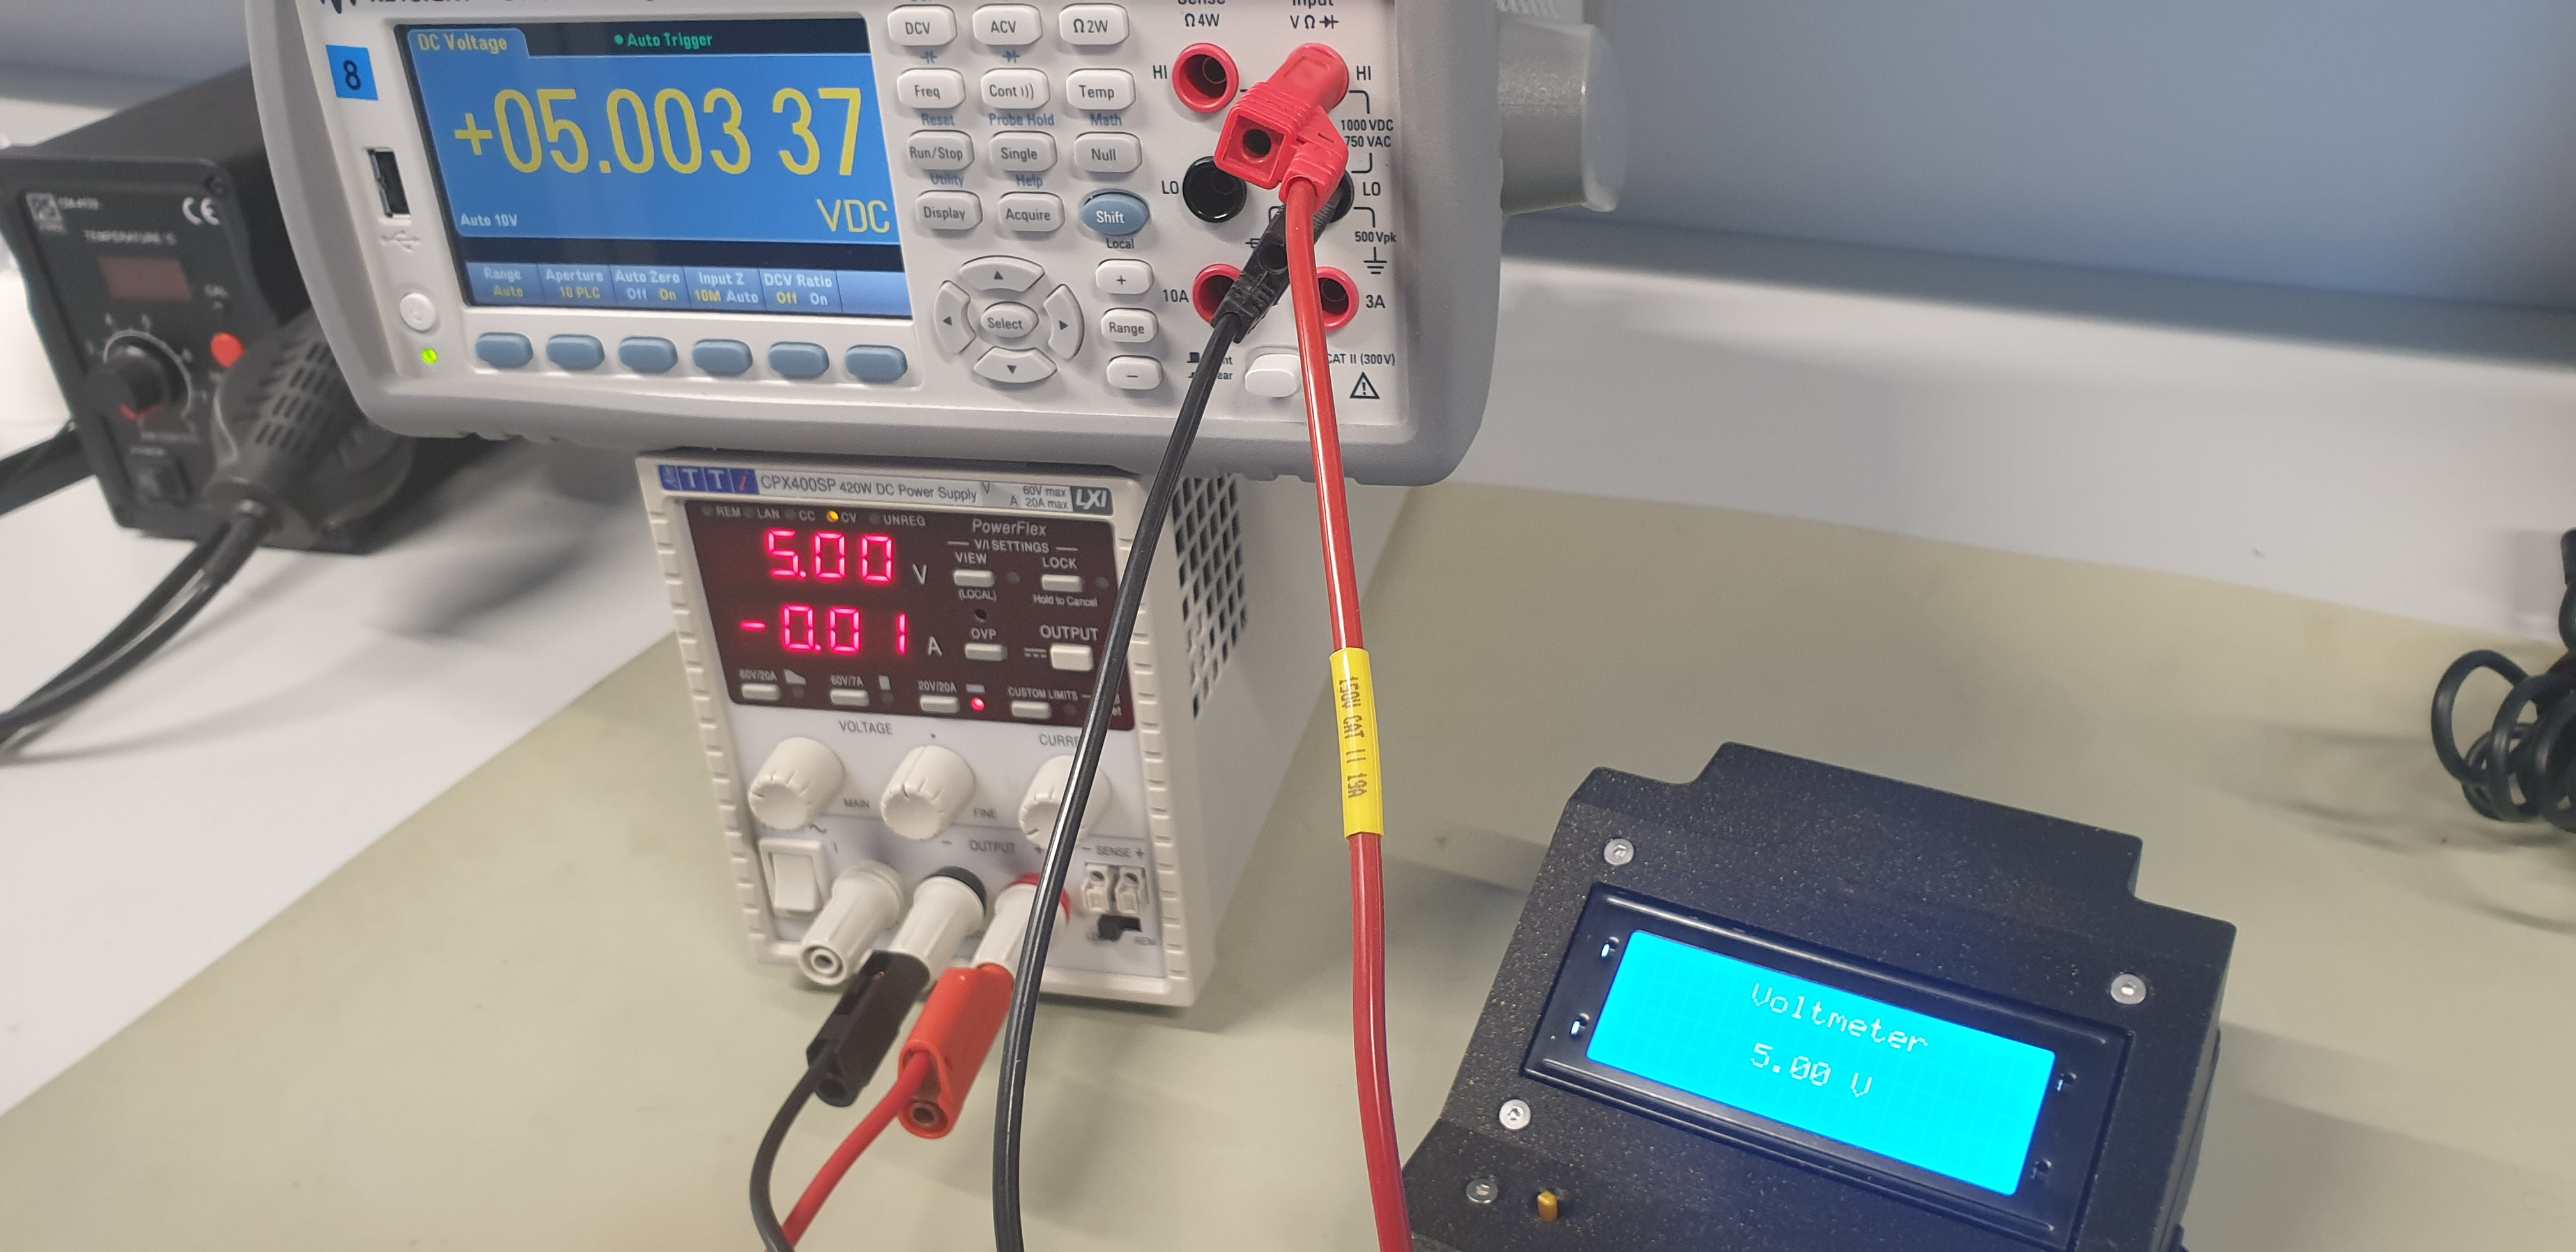
\includegraphics[height=5cm]{images/Measure/VTset.jpg}}
    \caption{Voltage test setup, showing 5V}
    \label{fig:VM1}
\end{figure}

\begin{figure}[h]
    \centering
    \frame{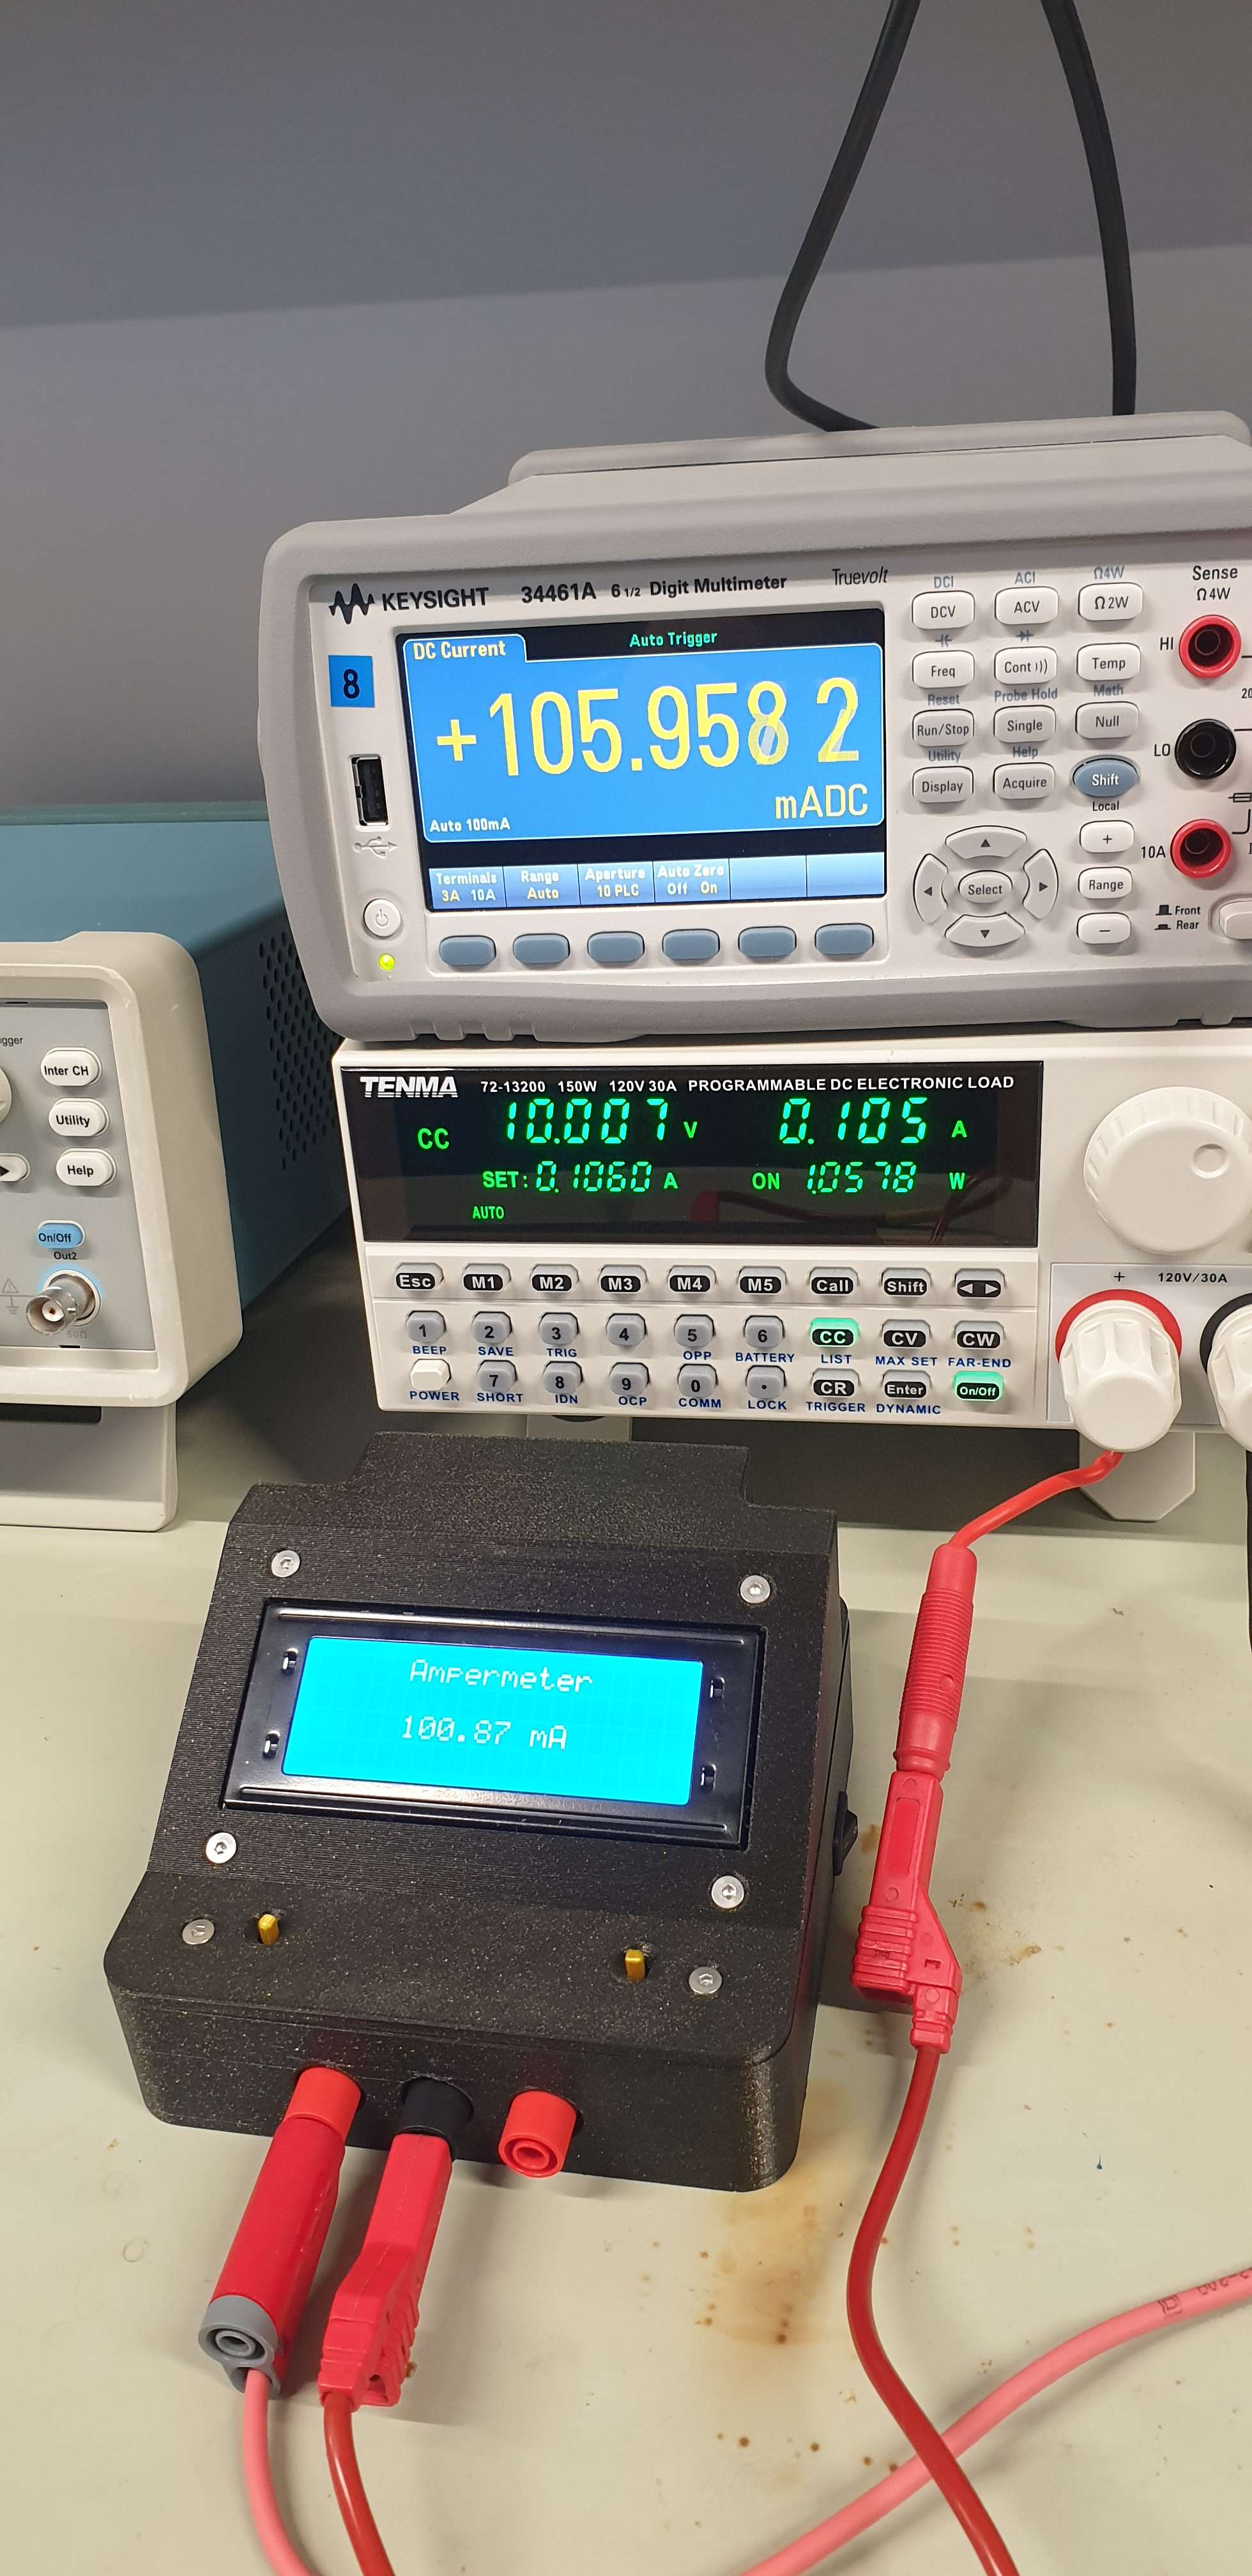
\includegraphics[height=7cm]{images//Measure/currMeas1.jpg}}
    \caption{Current test setup, min value}
    \label{fig:CM1}
\end{figure}

\begin{figure}[h]
    \centering
    \frame{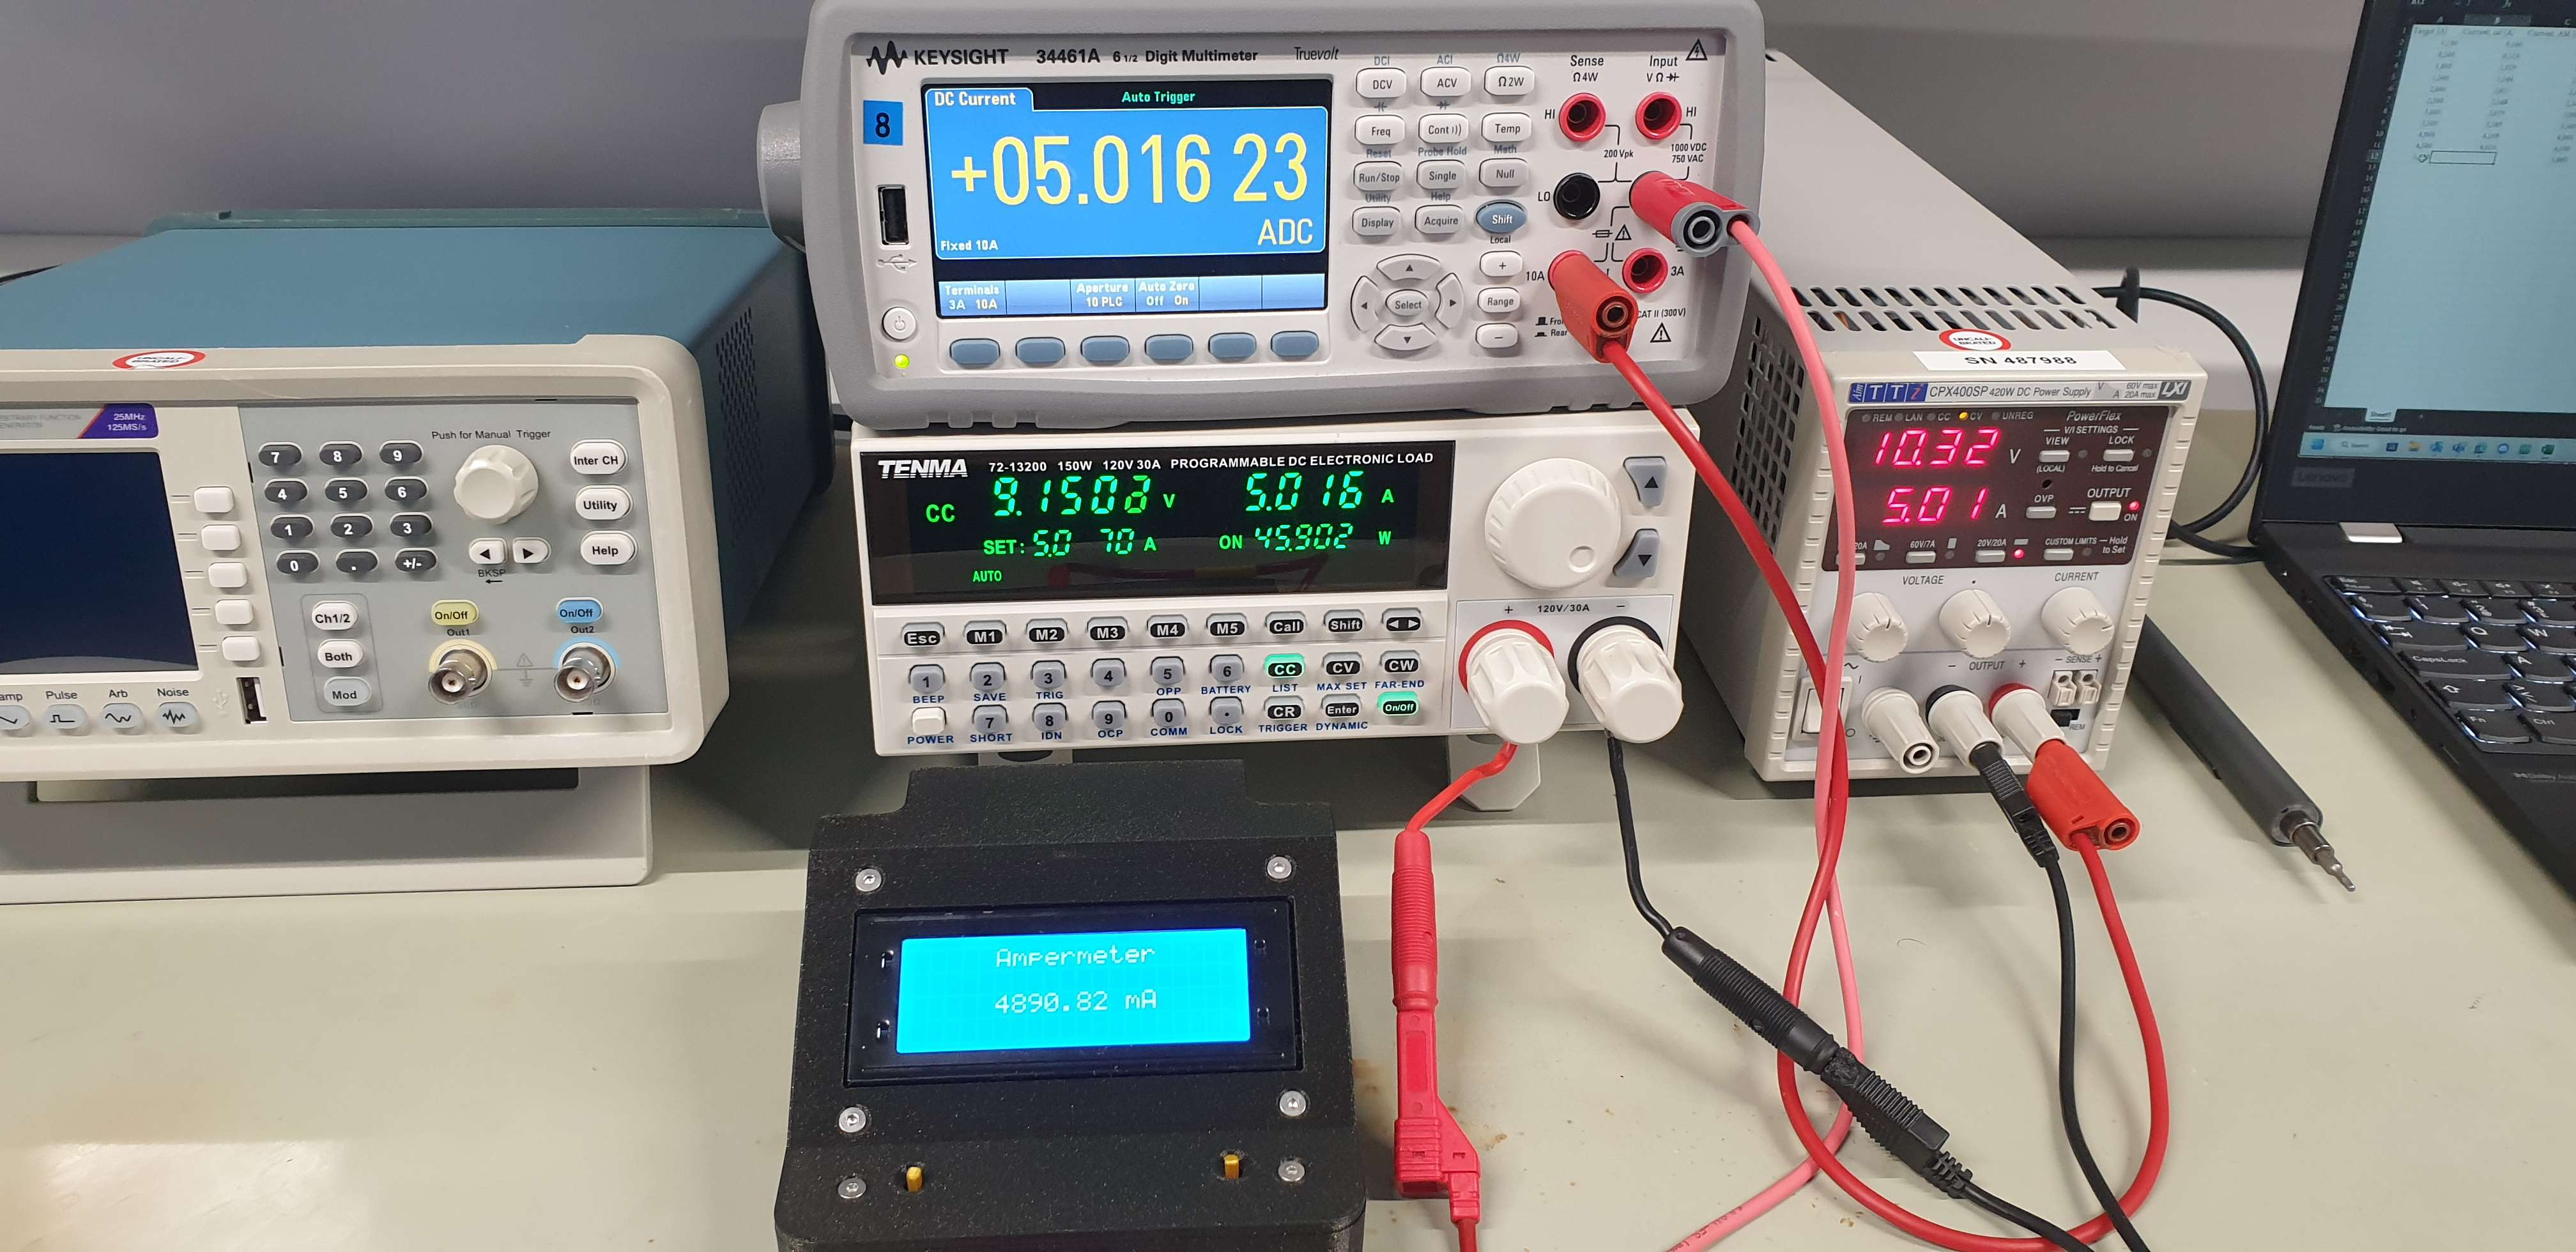
\includegraphics[height=5cm]{images//Measure/currMeas2.jpg}}
    \caption{Current test setup, max value}
    \label{fig:CM2}
\end{figure}

\begin{figure}[h]
    \centering
    \frame{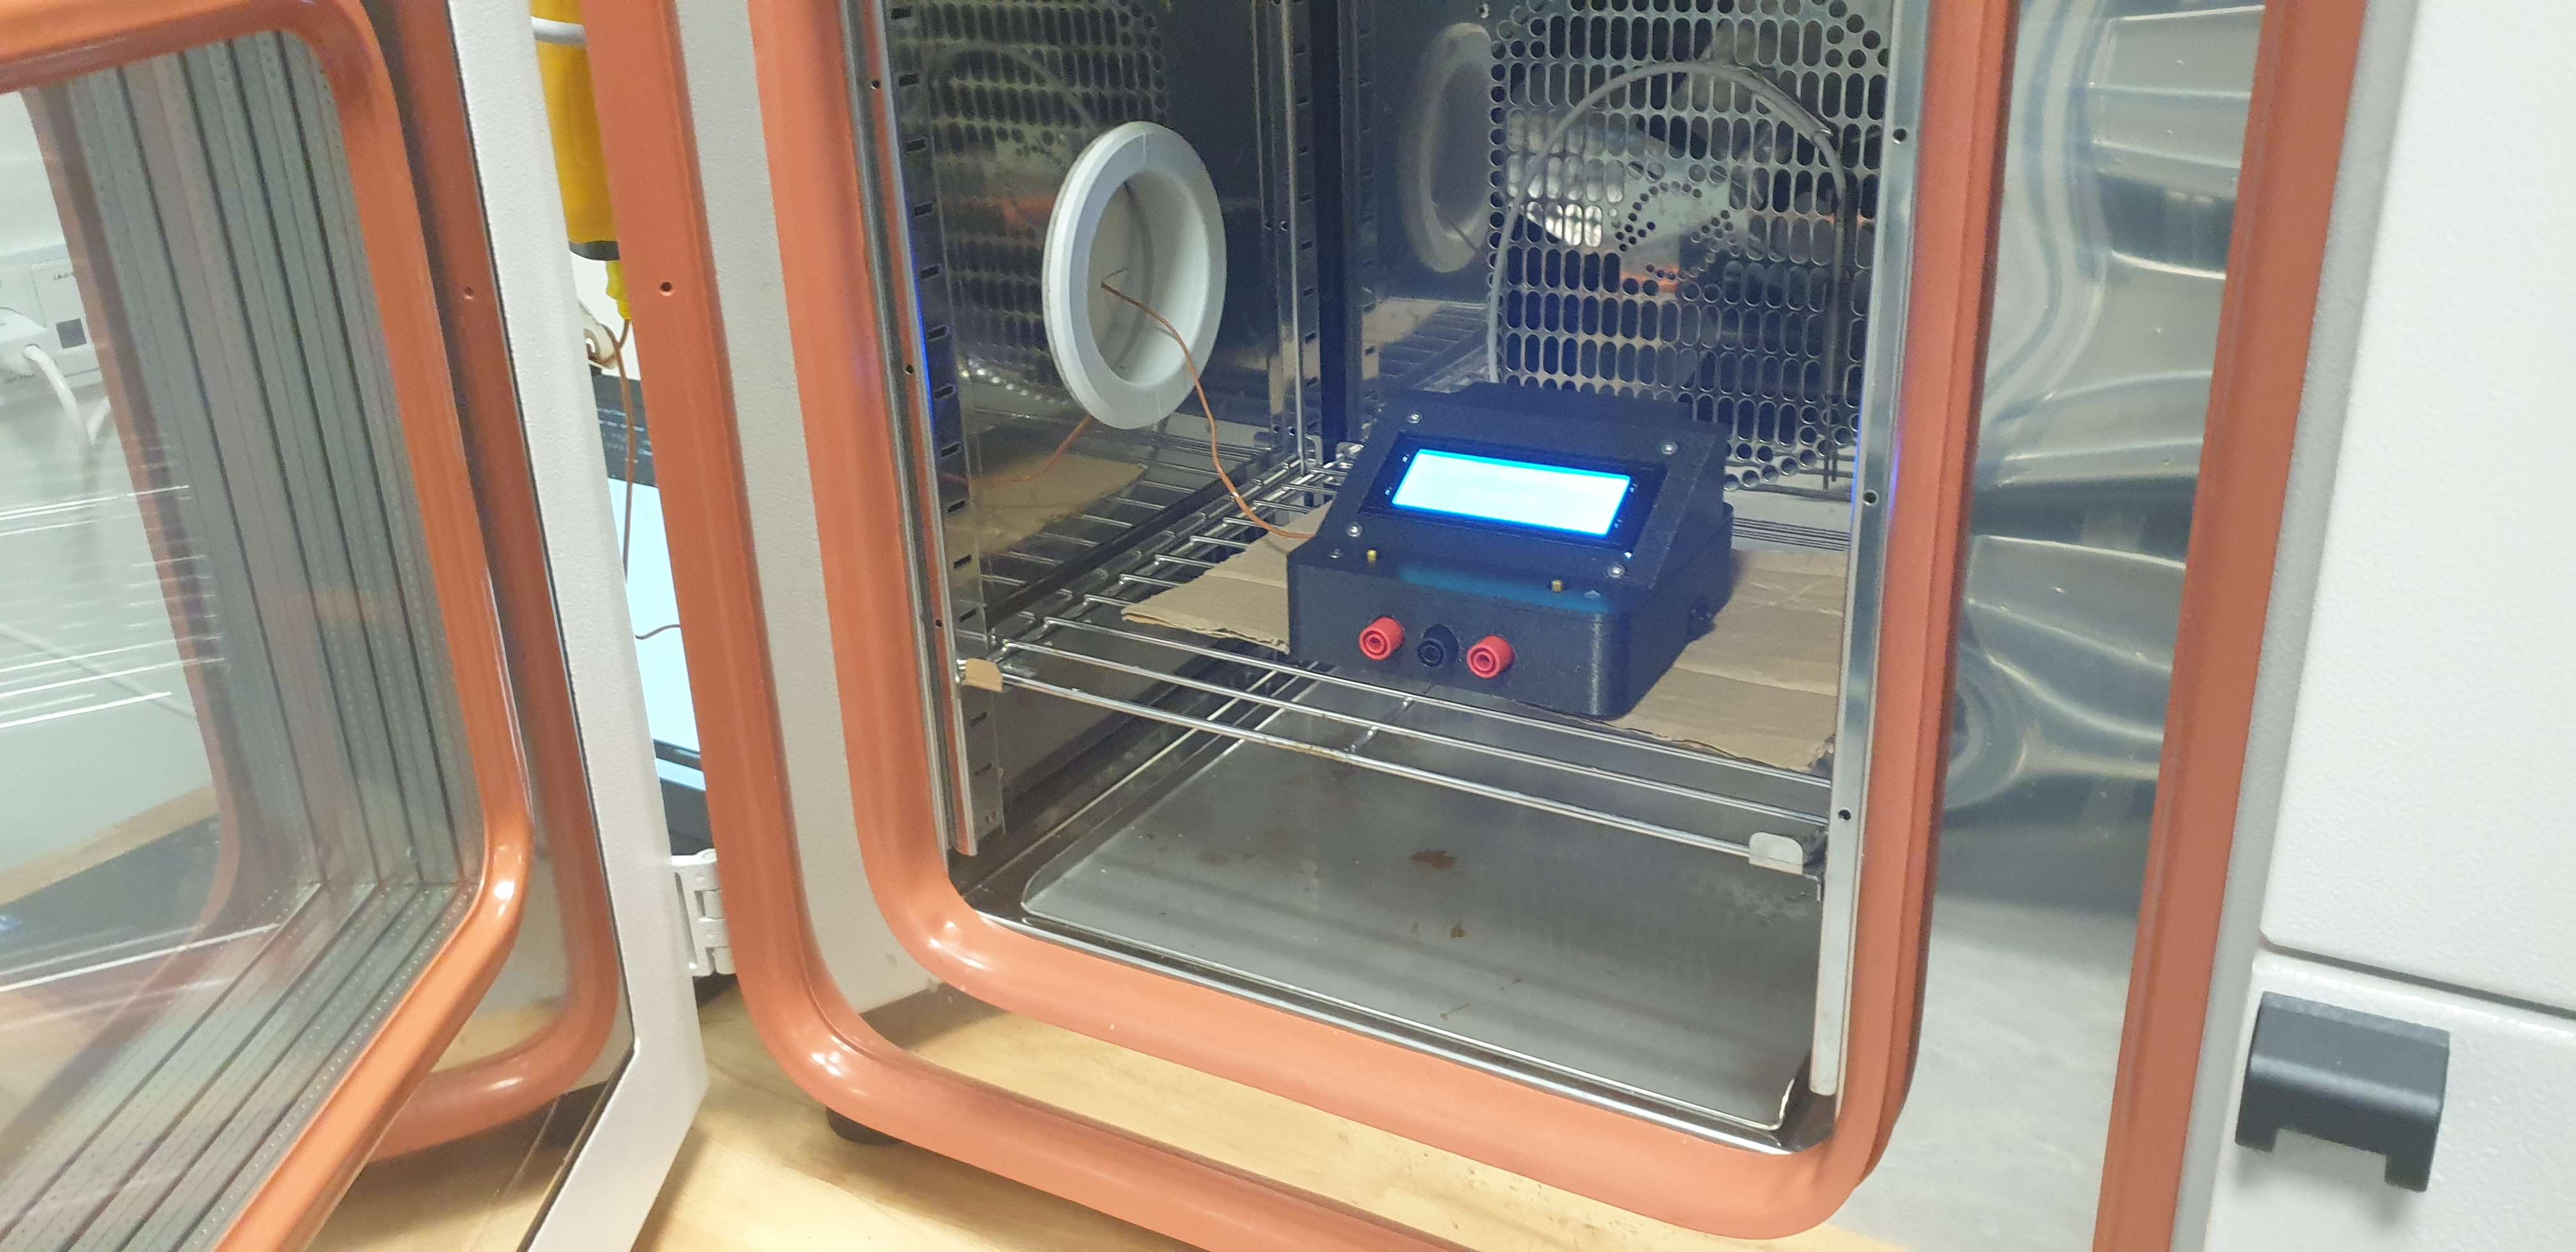
\includegraphics[height=6cm]{images/temp_test_setup.jpg}}
    \caption{Temperature test setup, inside}
    \label{fig:TM1}
\end{figure}

\begin{figure}[h]
    \centering
    \frame{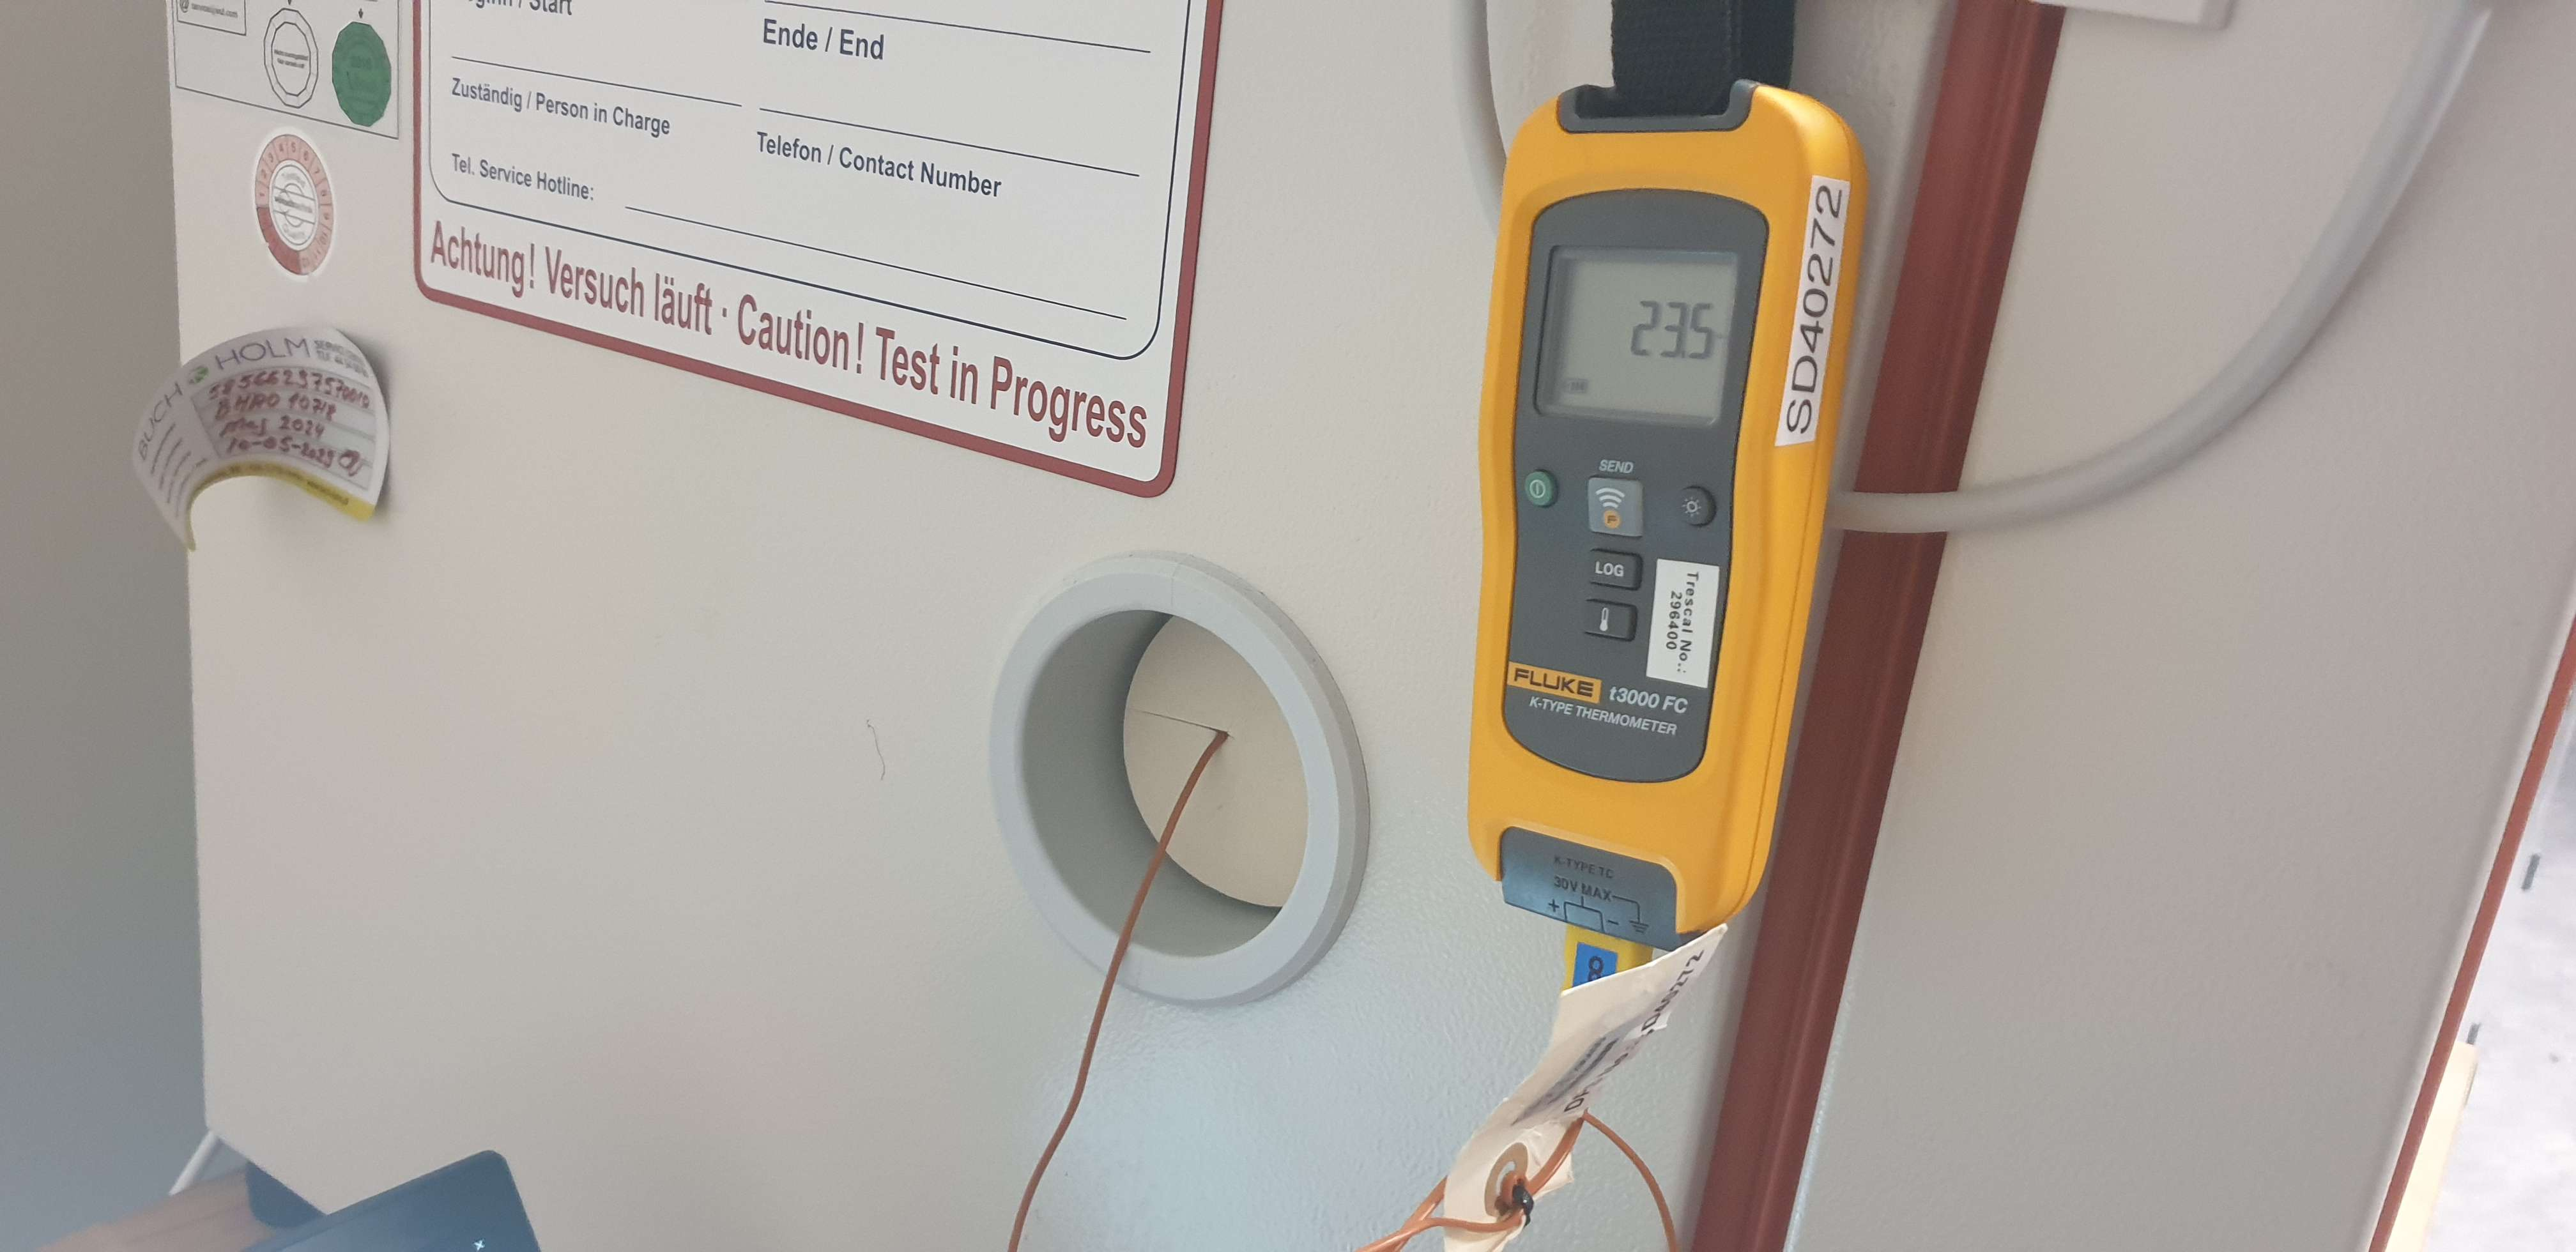
\includegraphics[height=6cm]{images/TSetup2.jpg}}
    \caption{Temperature test setup, outside}
    \label{fig:TM2}
\end{figure}

\begin{figure}[h]
    \centering
    \frame{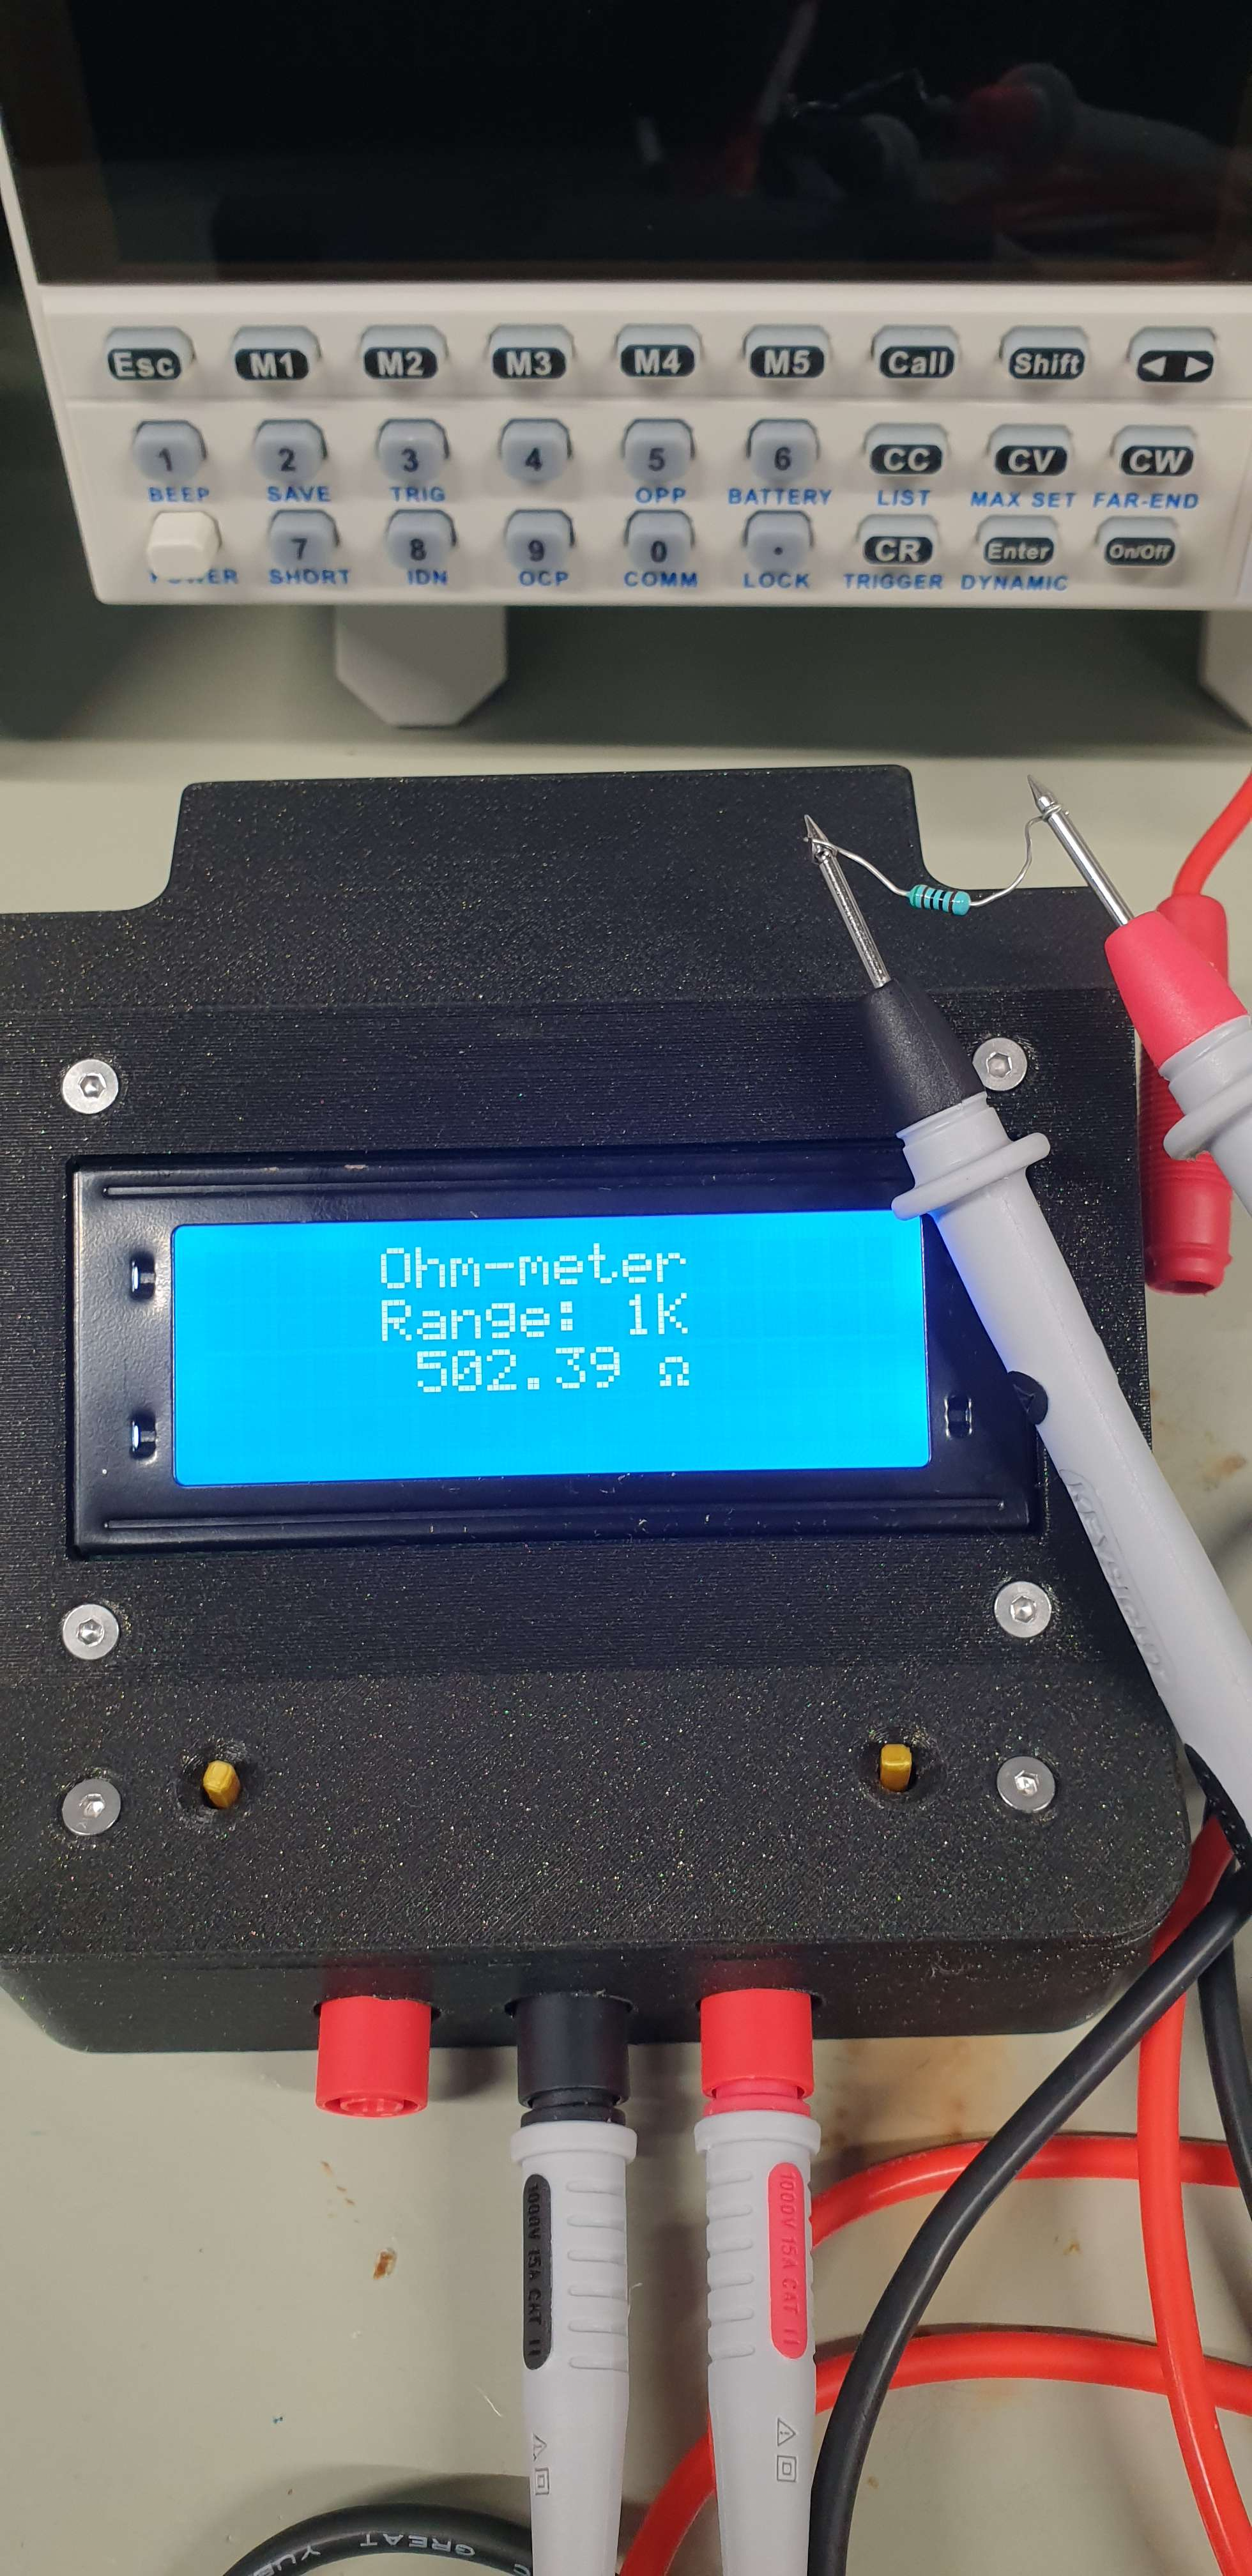
\includegraphics[height=7cm]{images//Measure/resMeas.jpg}}
    \caption{Resistance test setup, 510$\Omega$}
    \label{fig:RM1}
\end{figure}

\begin{figure}[h]
    \centering
    \frame{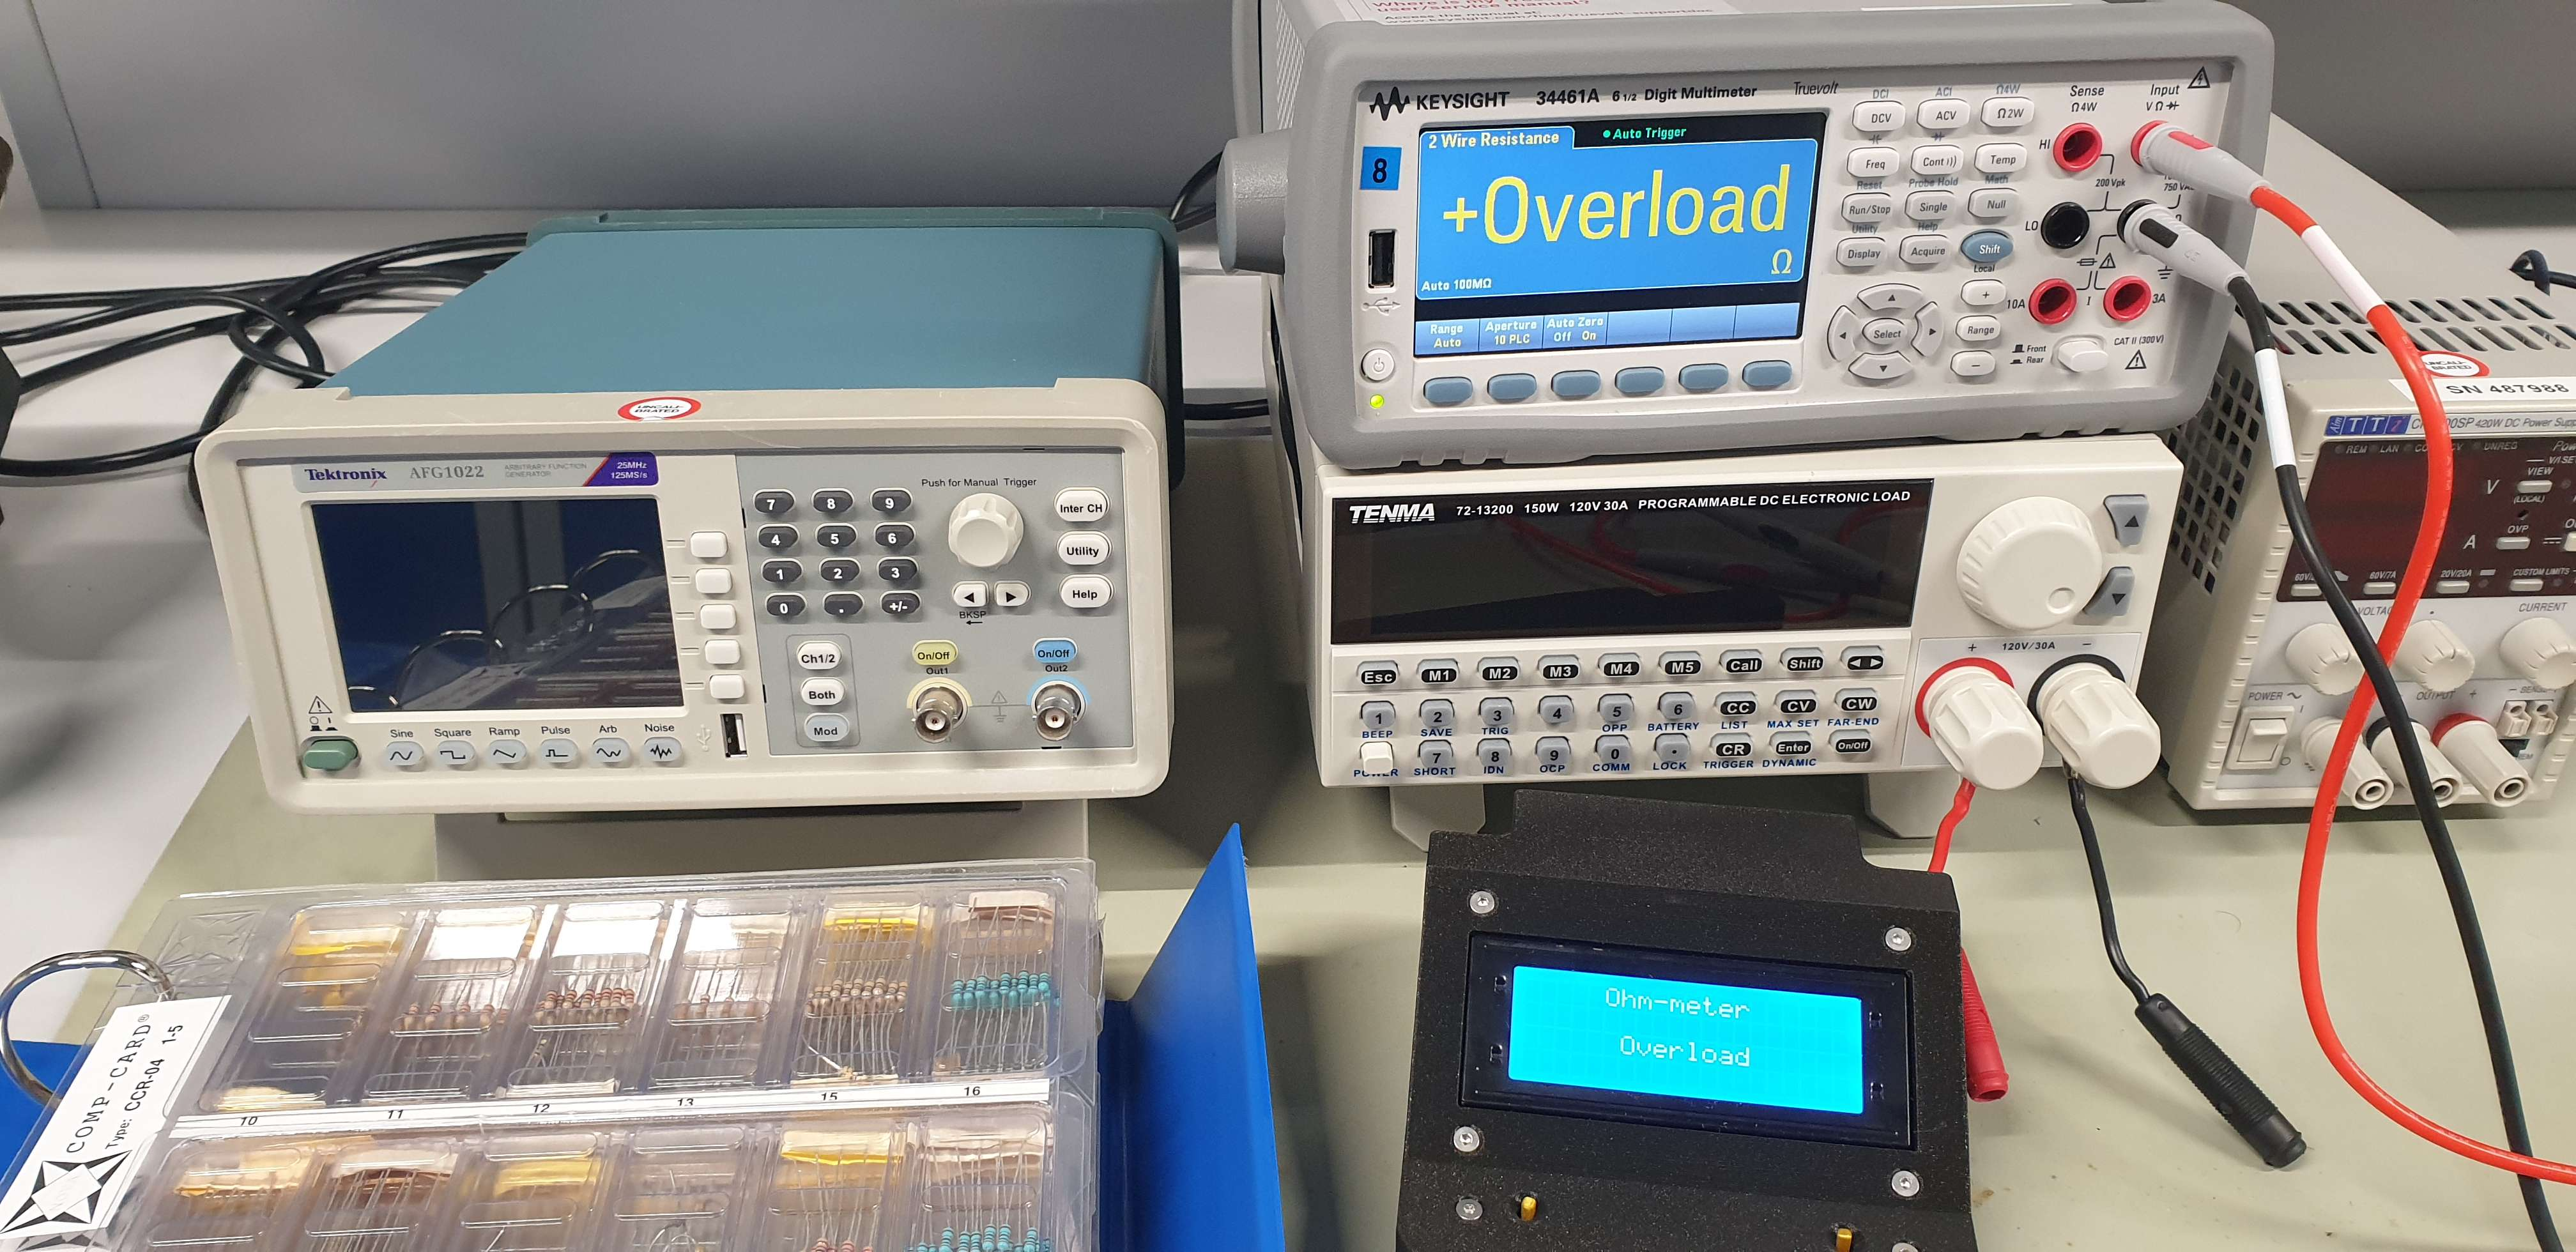
\includegraphics[height=5cm]{images//Measure/resMeas1.jpg}}
    \caption{Resistance test setup, with resistor assortment}
    \label{fig:RM2}
\end{figure}

\begin{figure}[h]
    \centering
    \frame{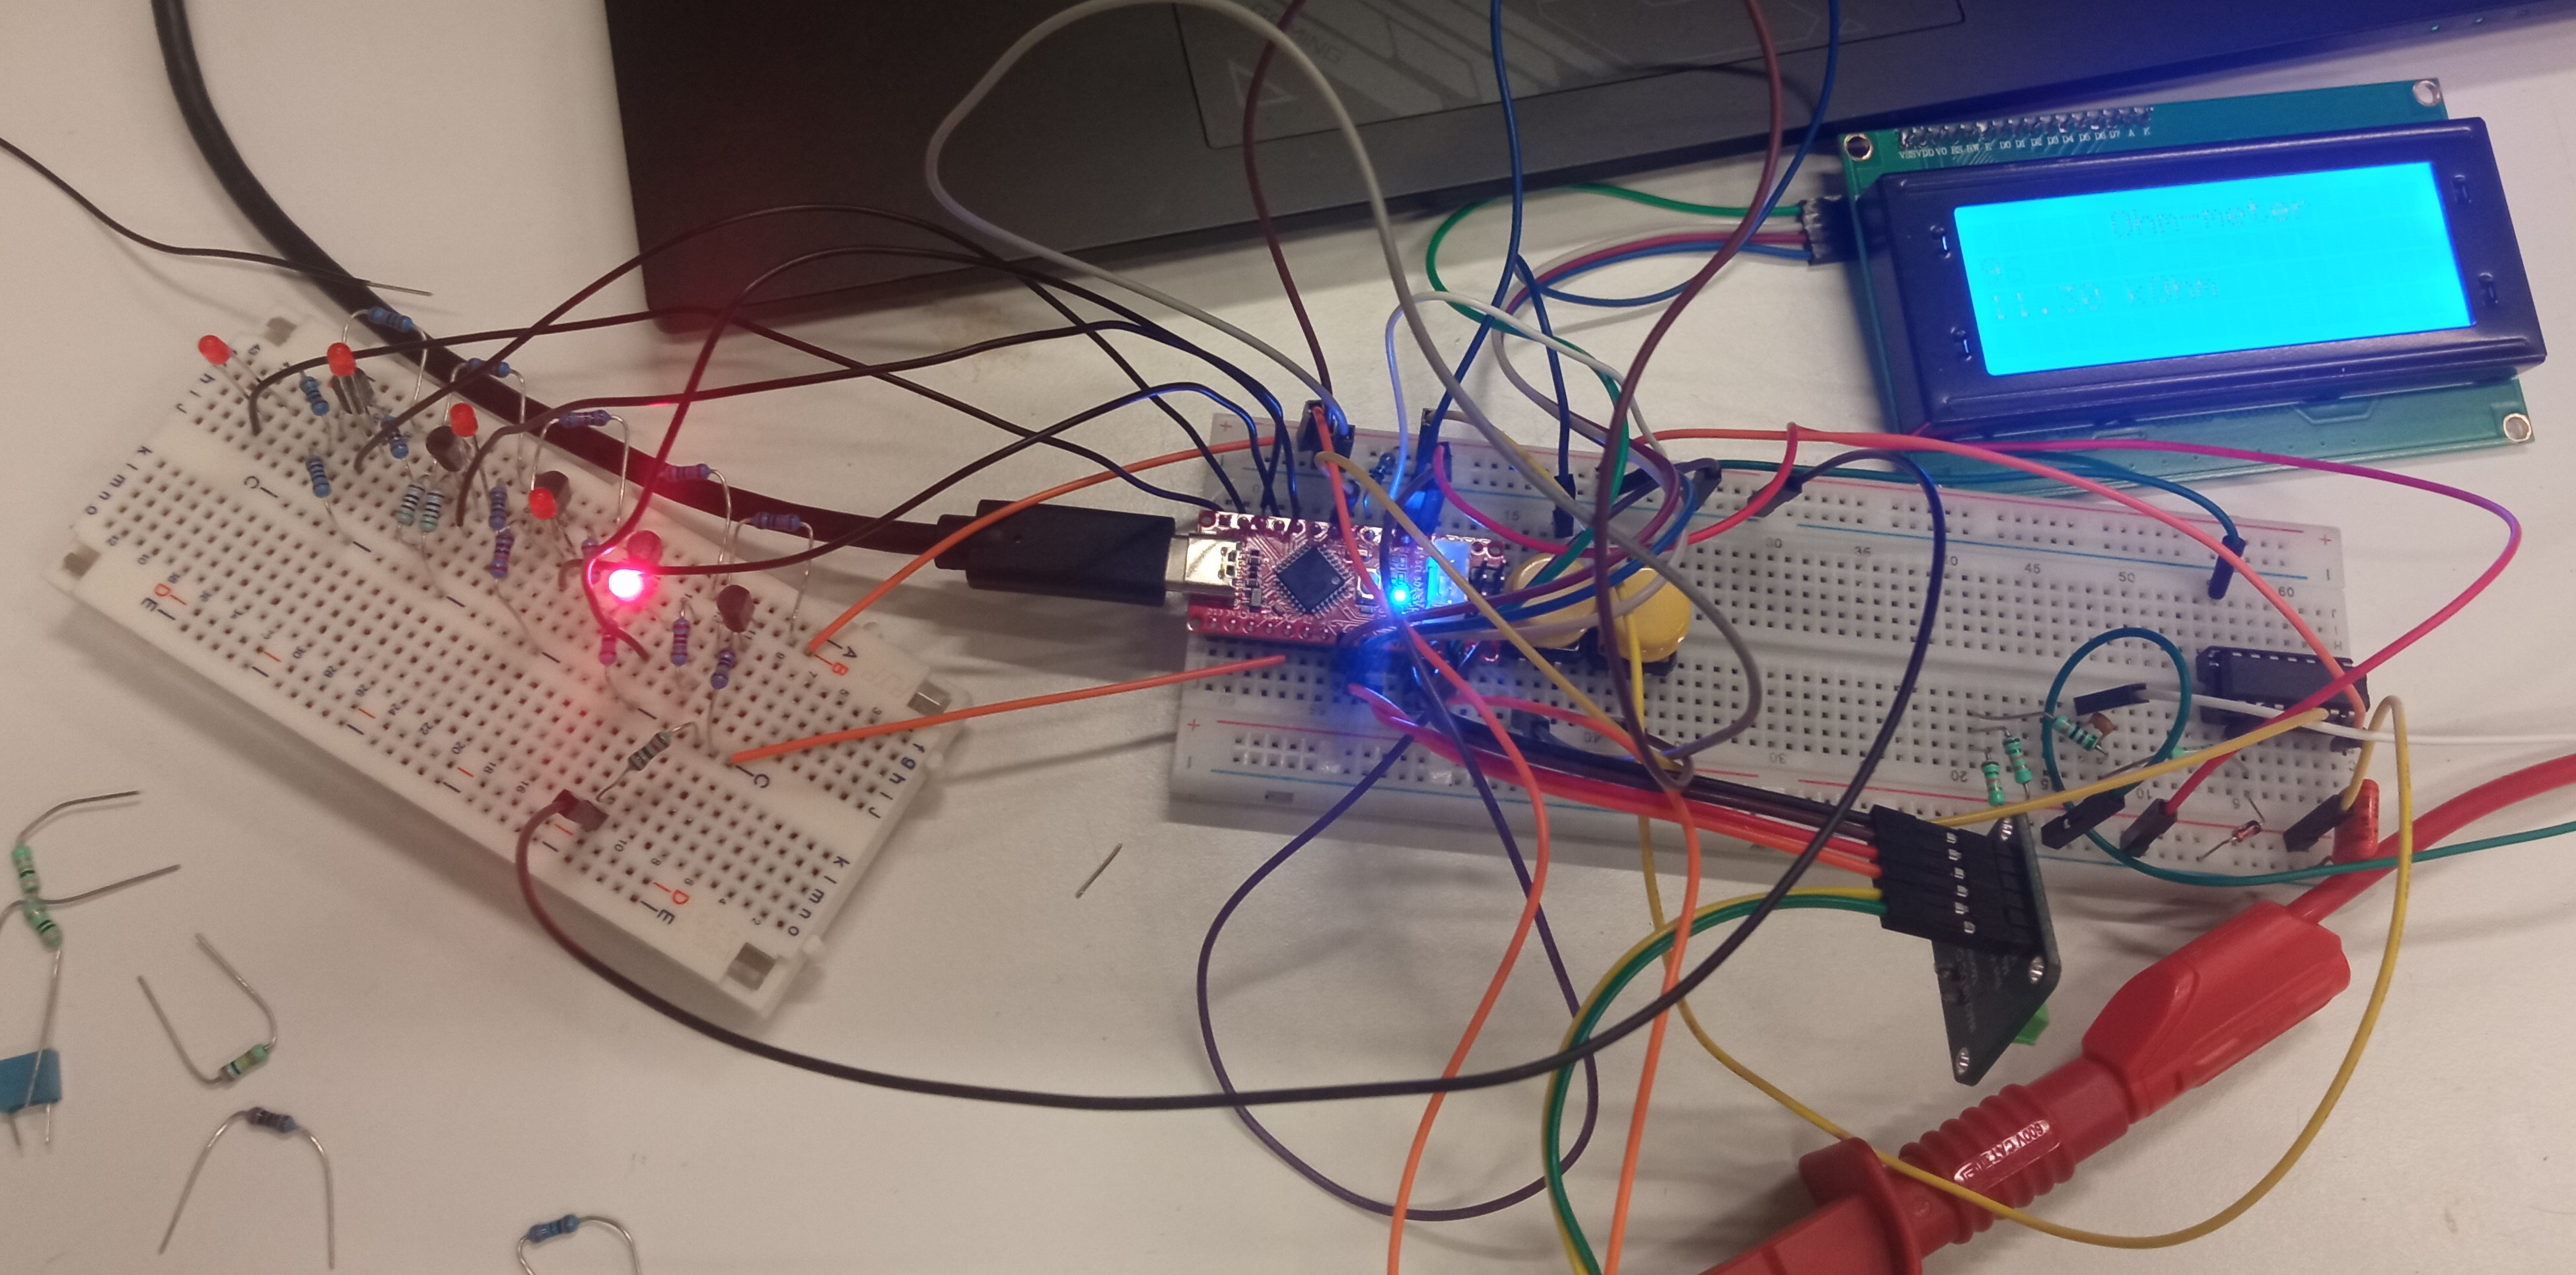
\includegraphics[height=6cm]{images/breadboard_proto.jpg}}
    \caption{Breadboard prototyping}
    \label{fig:breadboardPrototyping}
\end{figure}

\begin{figure}[h]
    \centering
    \frame{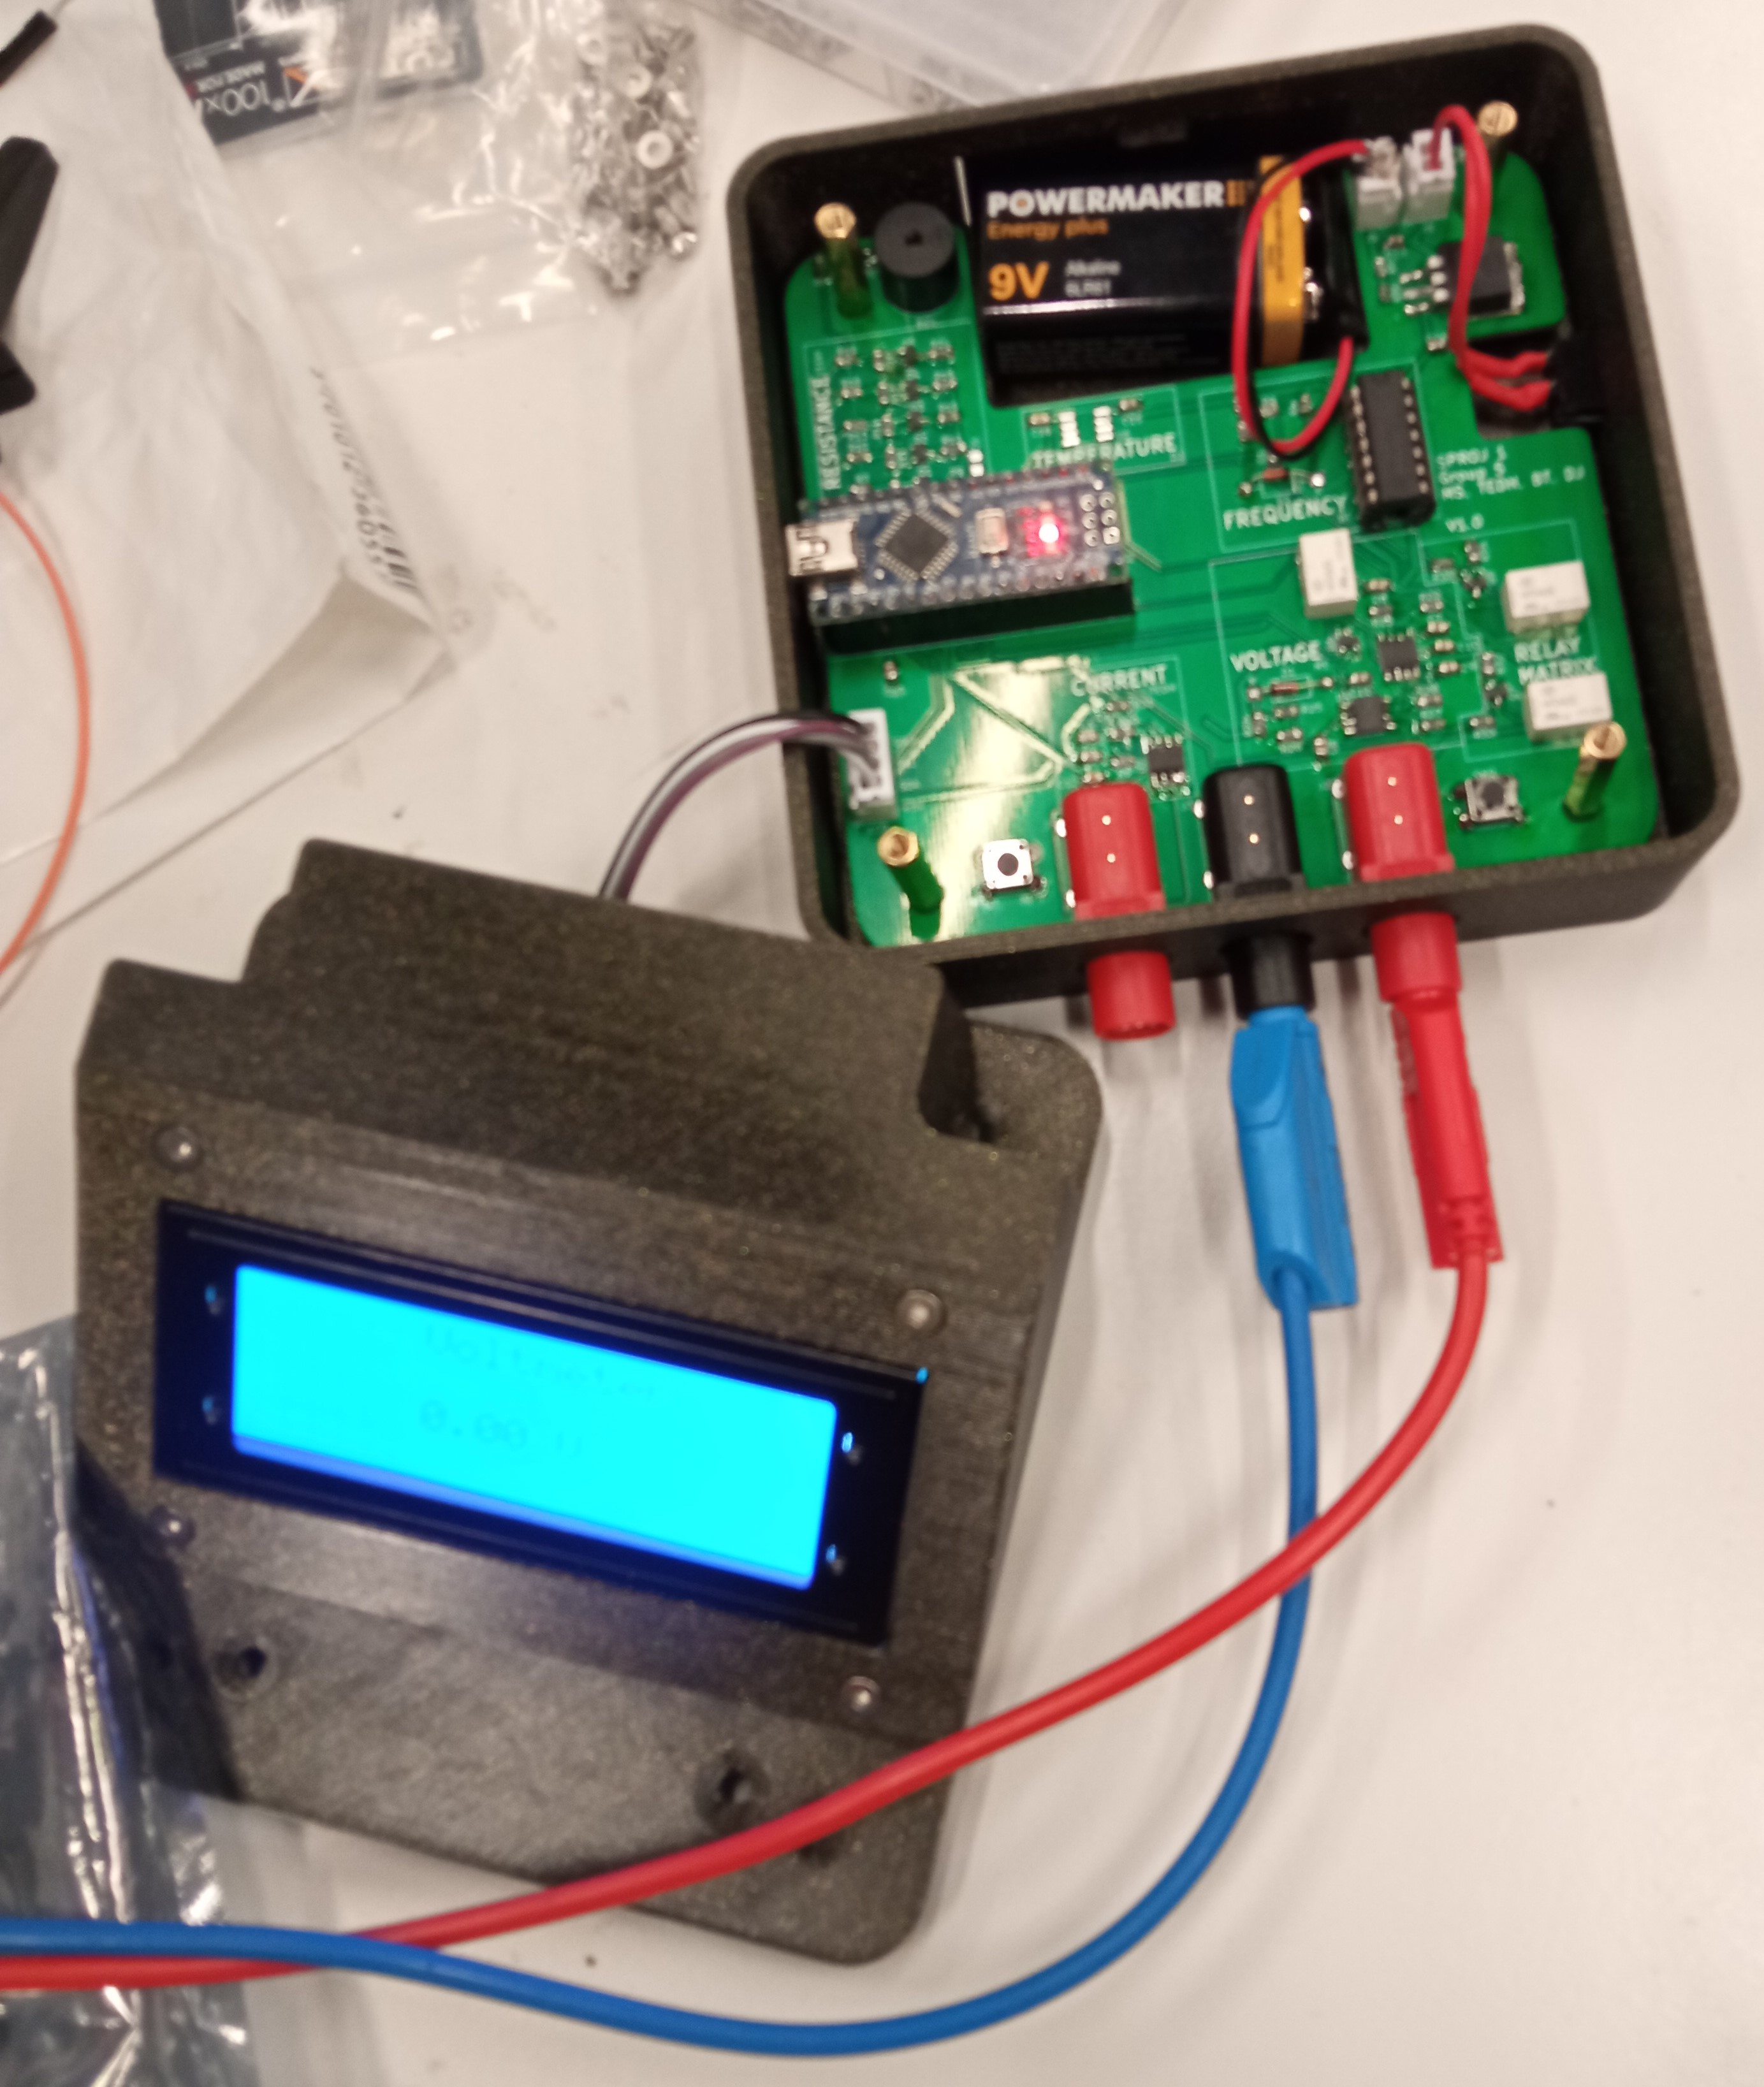
\includegraphics[height=8cm]{images/MM_V1.jpg}}
    \caption{Multimeter V1.0 during testing}
    \label{fig:MMV1}
\end{figure}

\begin{figure}[h]
    \centering
    \frame{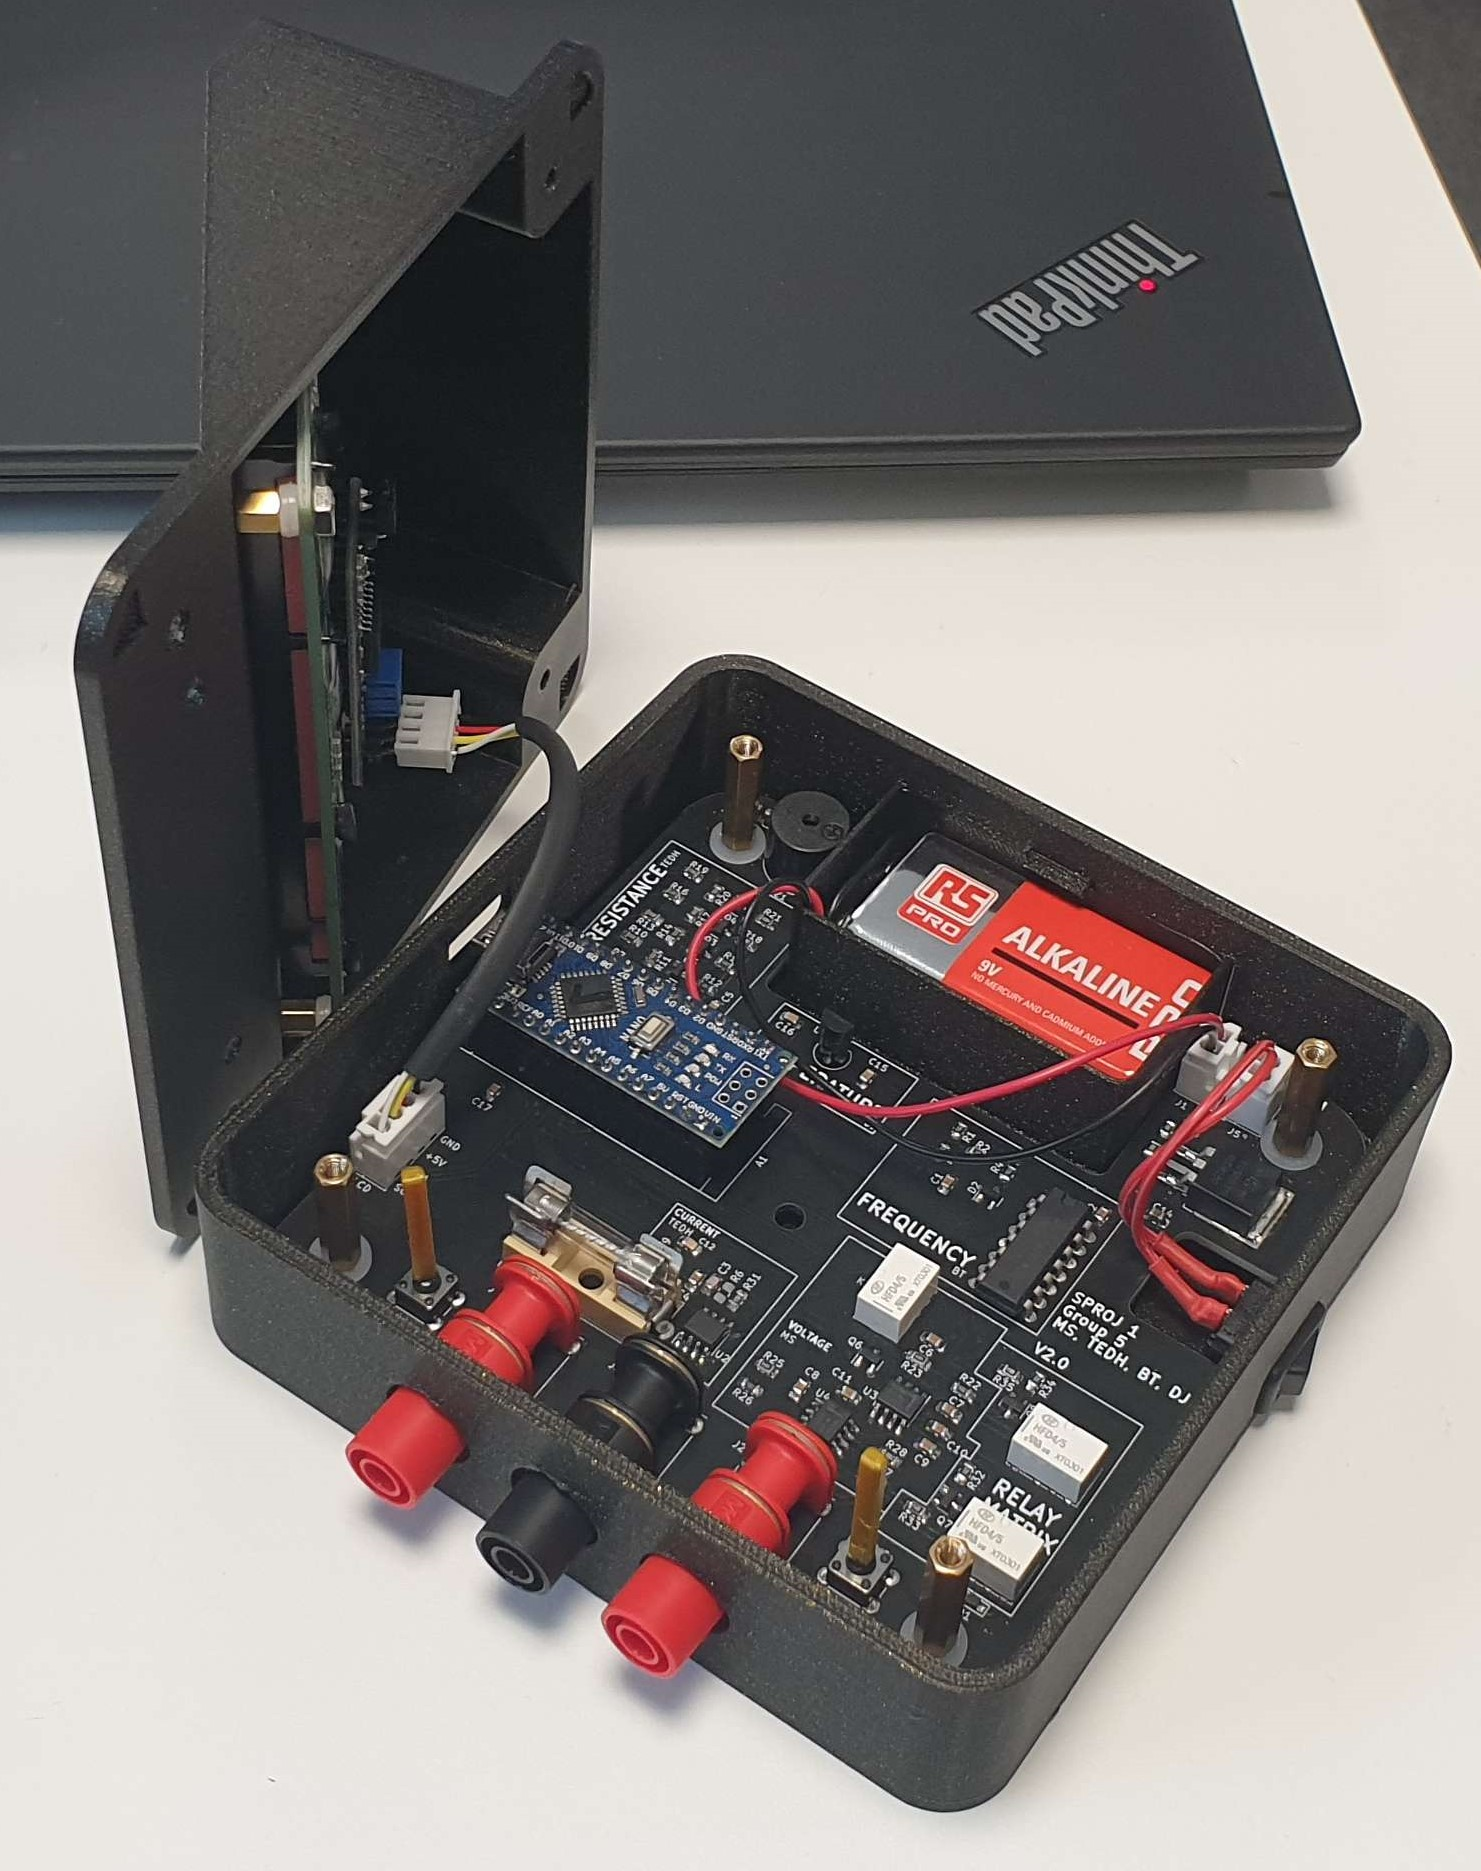
\includegraphics[height=8cm]{images/MM_Final.jpg}}
    \caption{Multimeter, final iteration}
    \label{fig:MM_final}
\end{figure}

\begin{figure}[h]
    \centering
    \frame{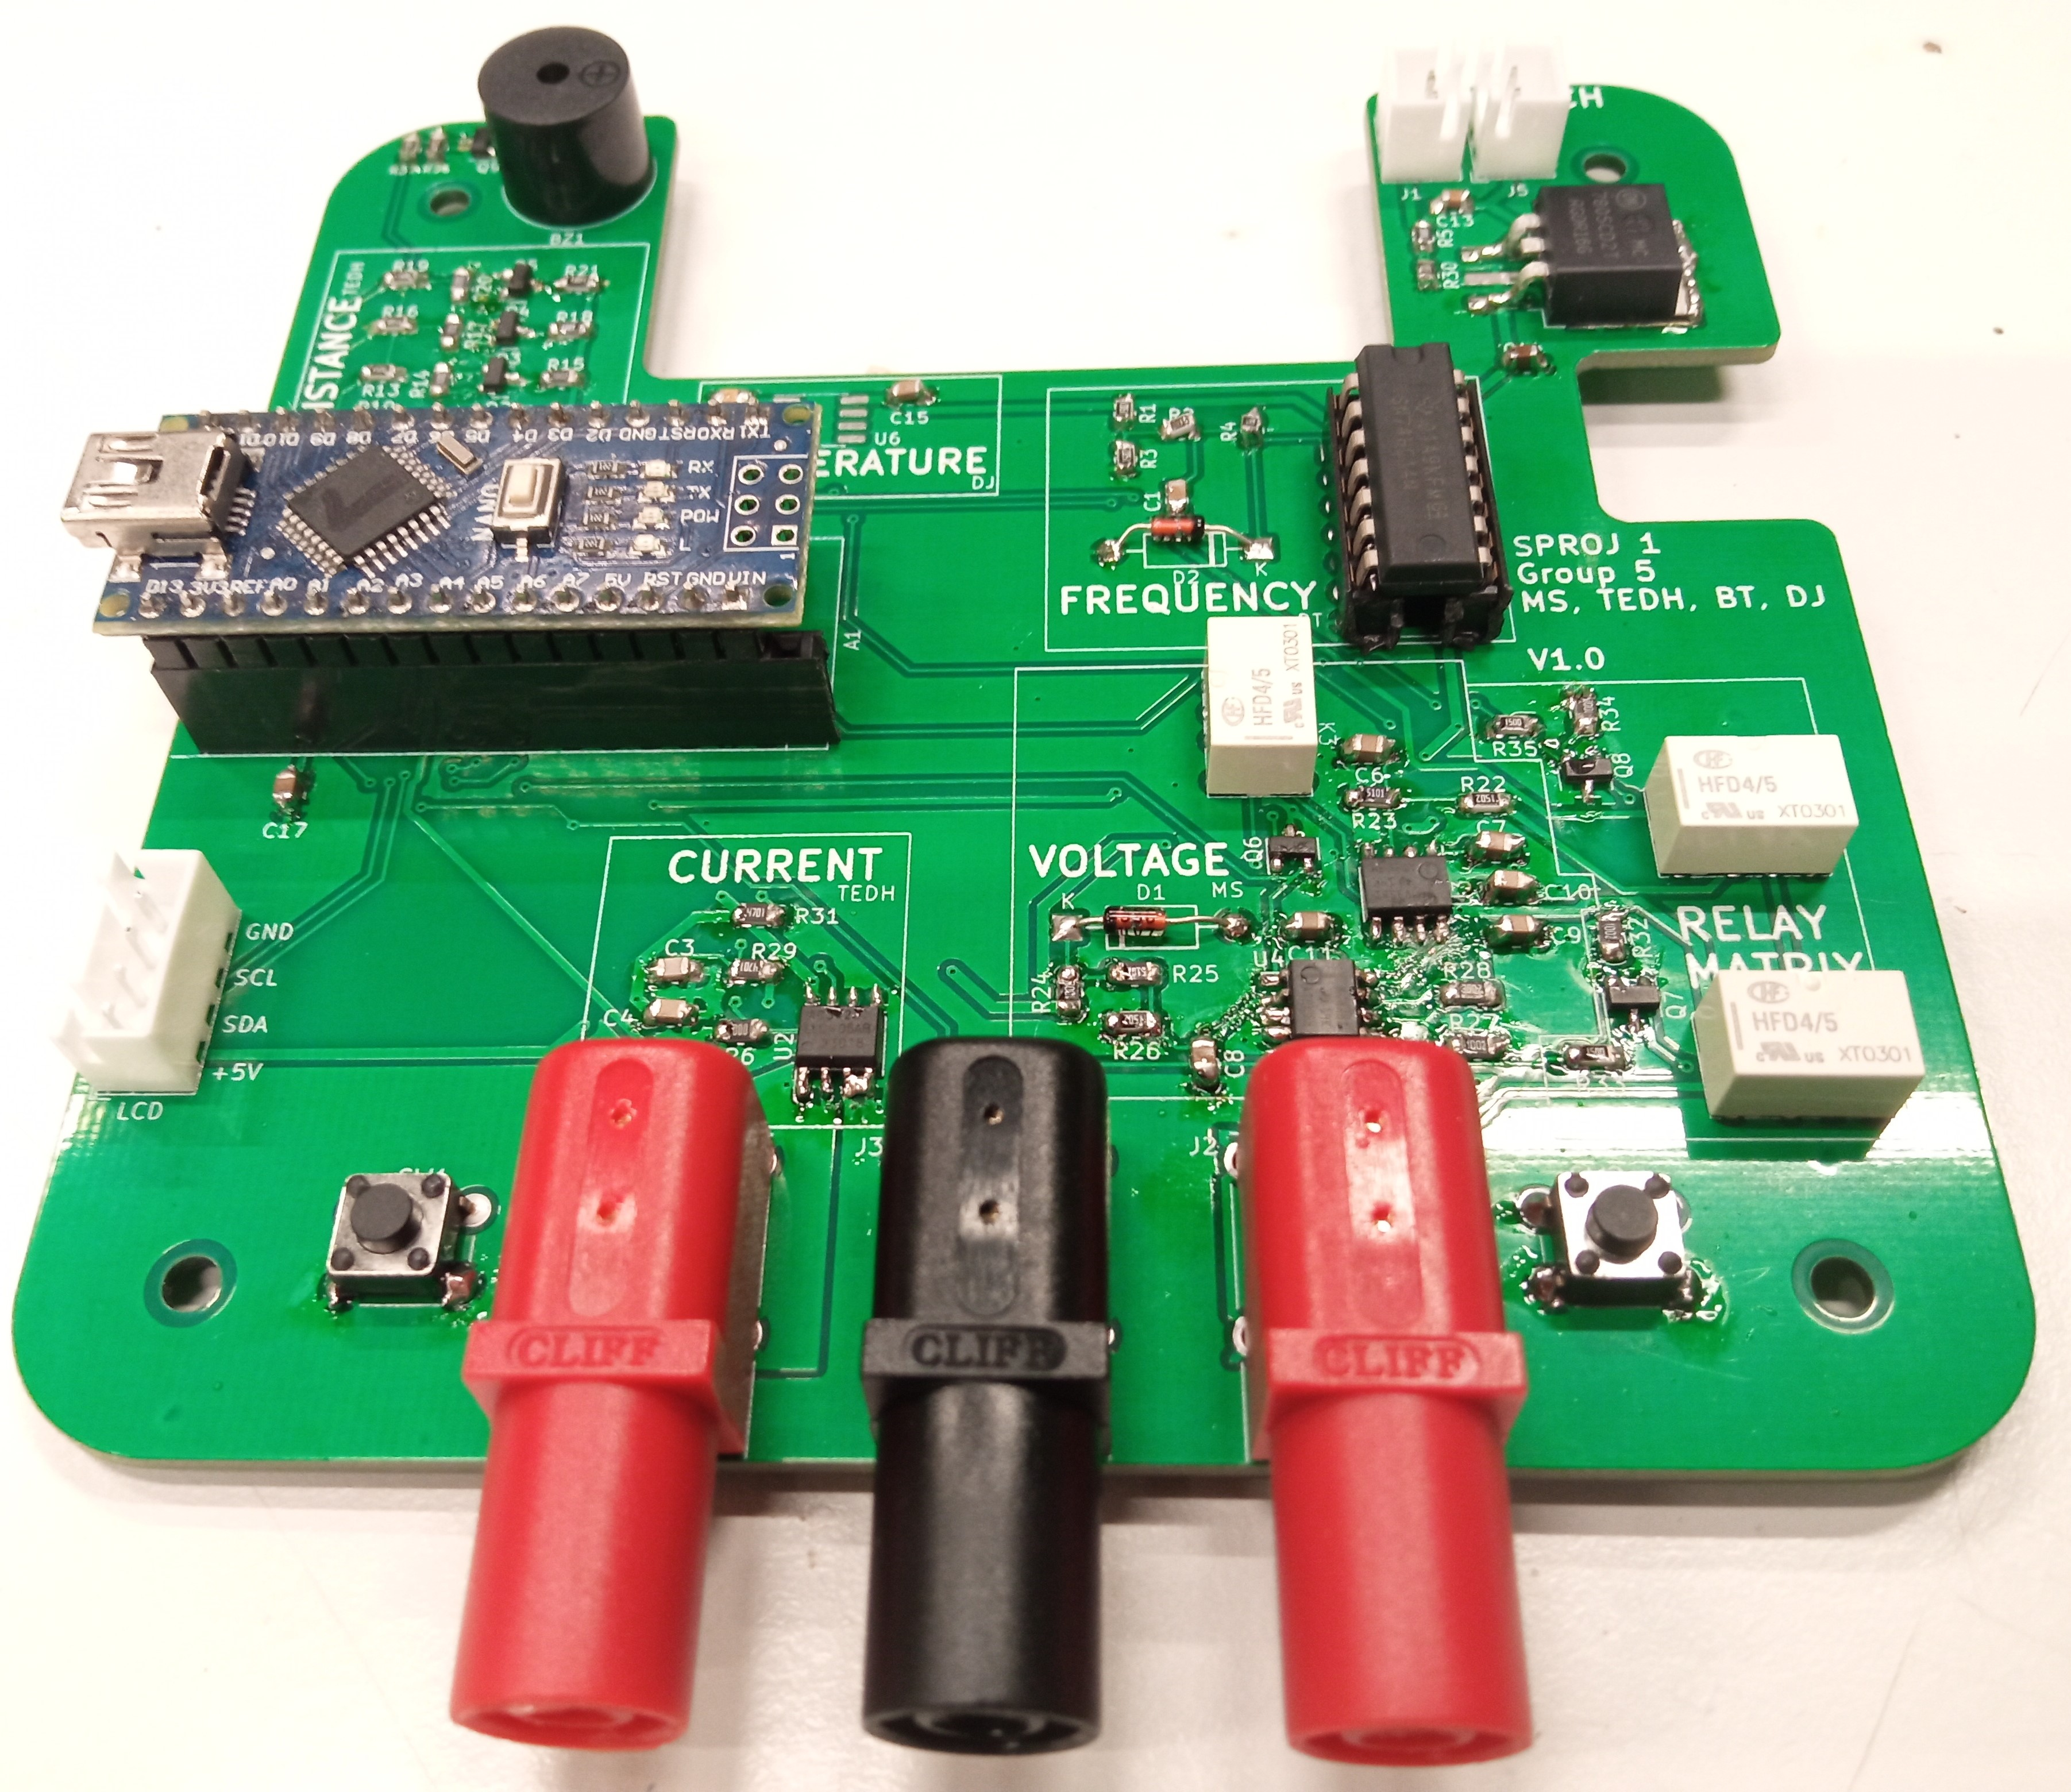
\includegraphics[height=7cm]{images/pcb_v1.jpg}}
    \caption{PCB Version V1.0}
    \label{fig:pcbV1}
\end{figure}

\begin{figure}[h]
    \centering
    \frame{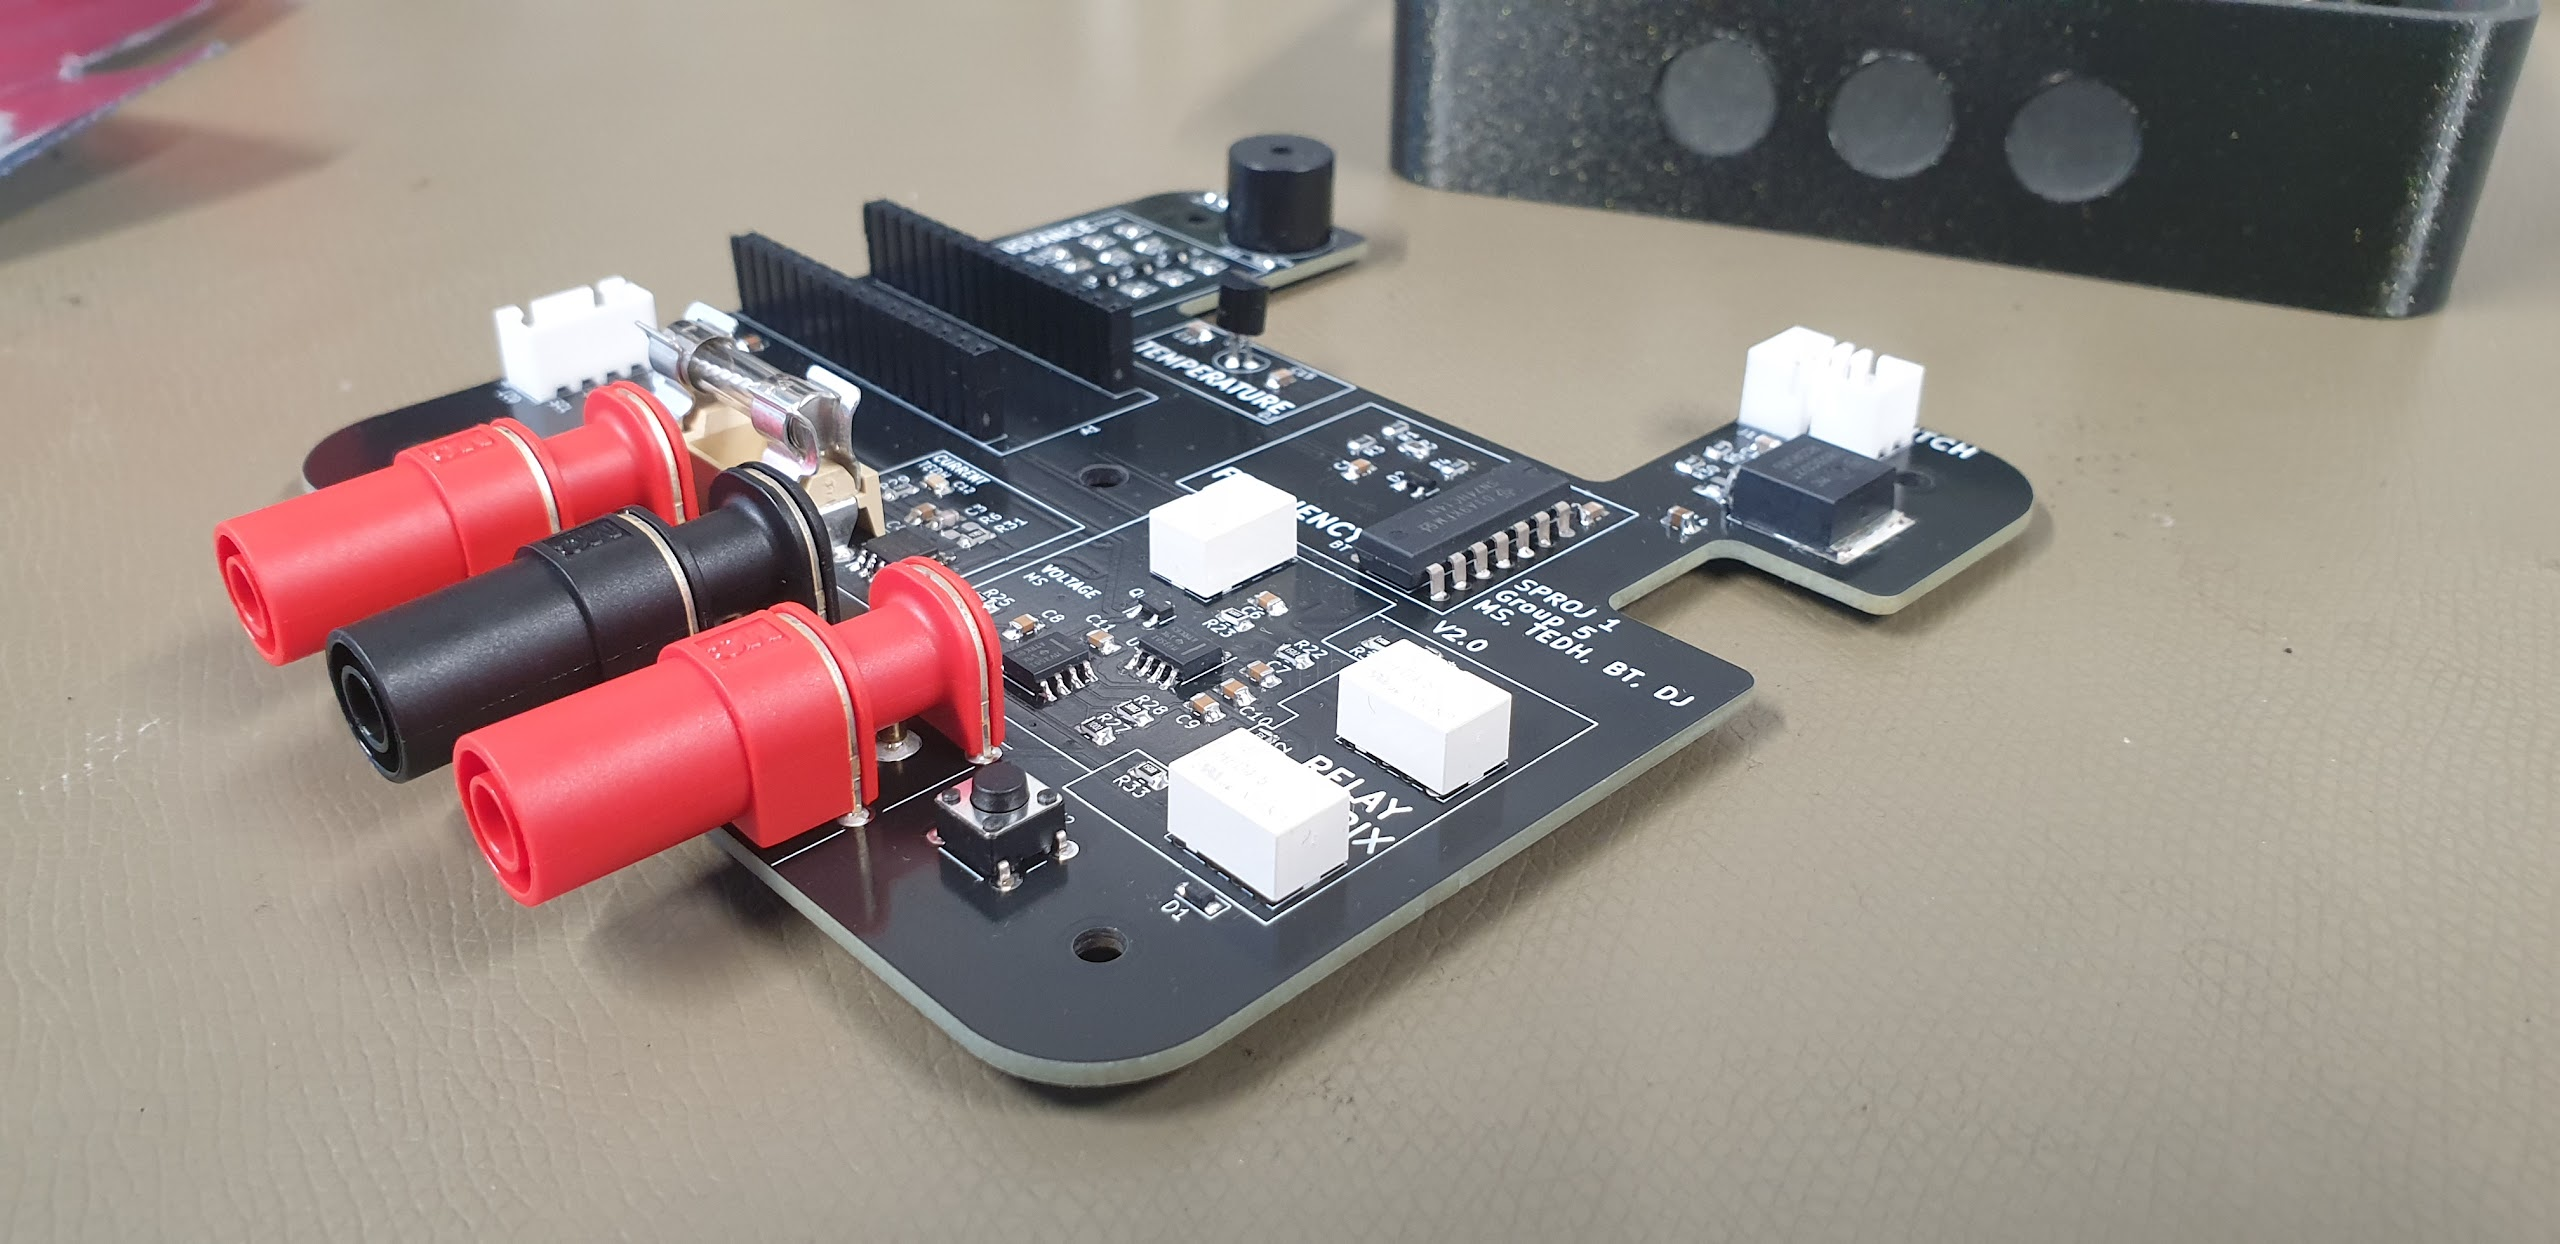
\includegraphics[width=1\linewidth]{images/PCB2.0V.jpg}}
    \caption{PCB Version V2.0}
    \label{fig:pcbV1}
\end{figure}

\begin{figure}[h]
    \centering
    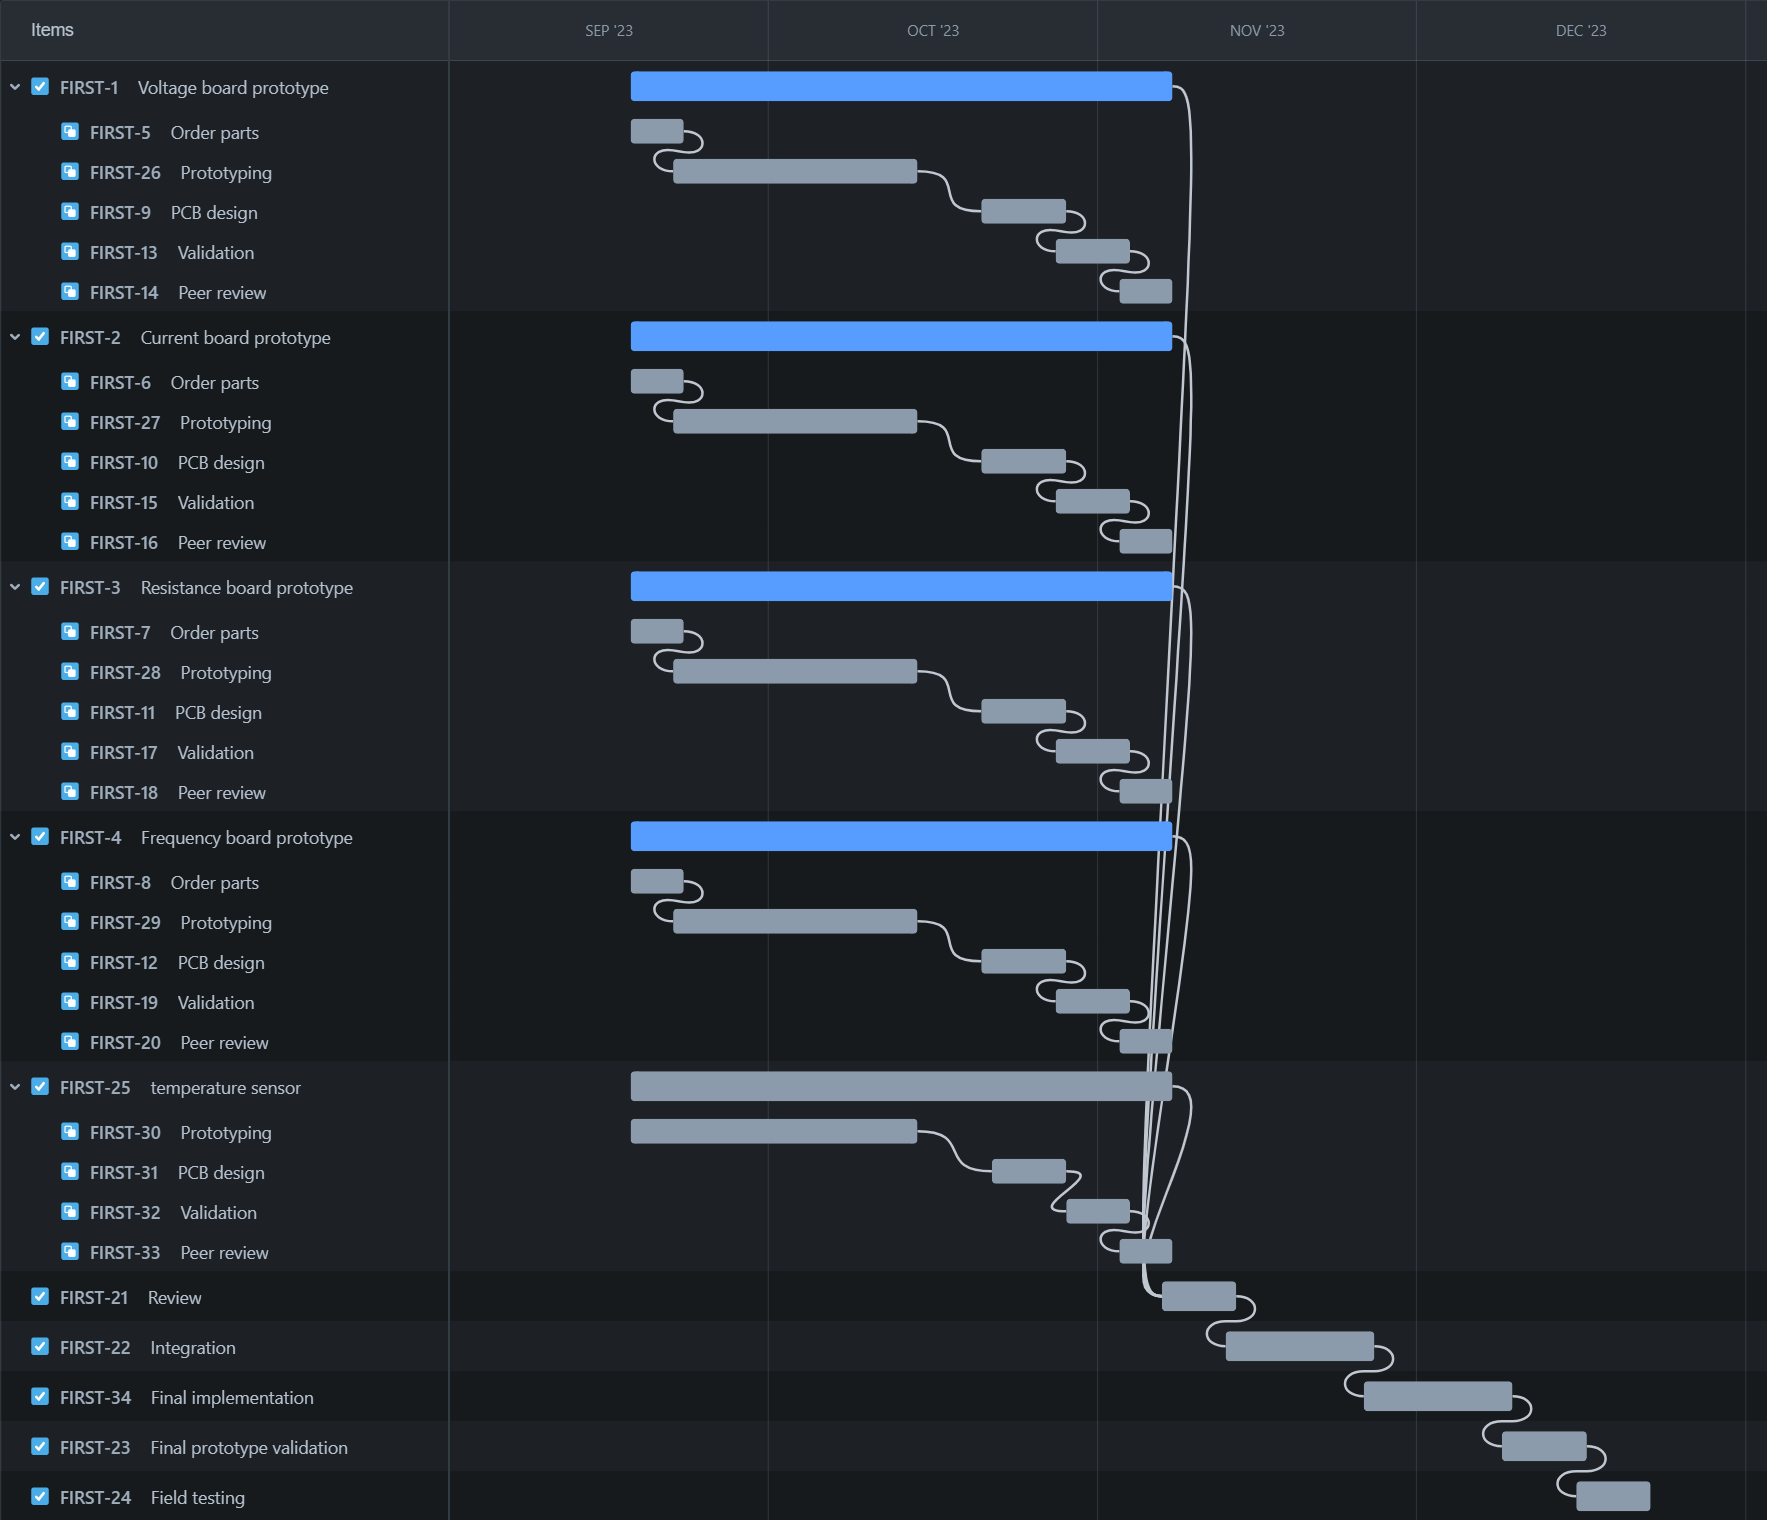
\includegraphics[width=1\linewidth]{images/SPROJ1G5_Timeline.png}
    \caption{Time plan}
    \label{fig:TP}
\end{figure}

\clearpage

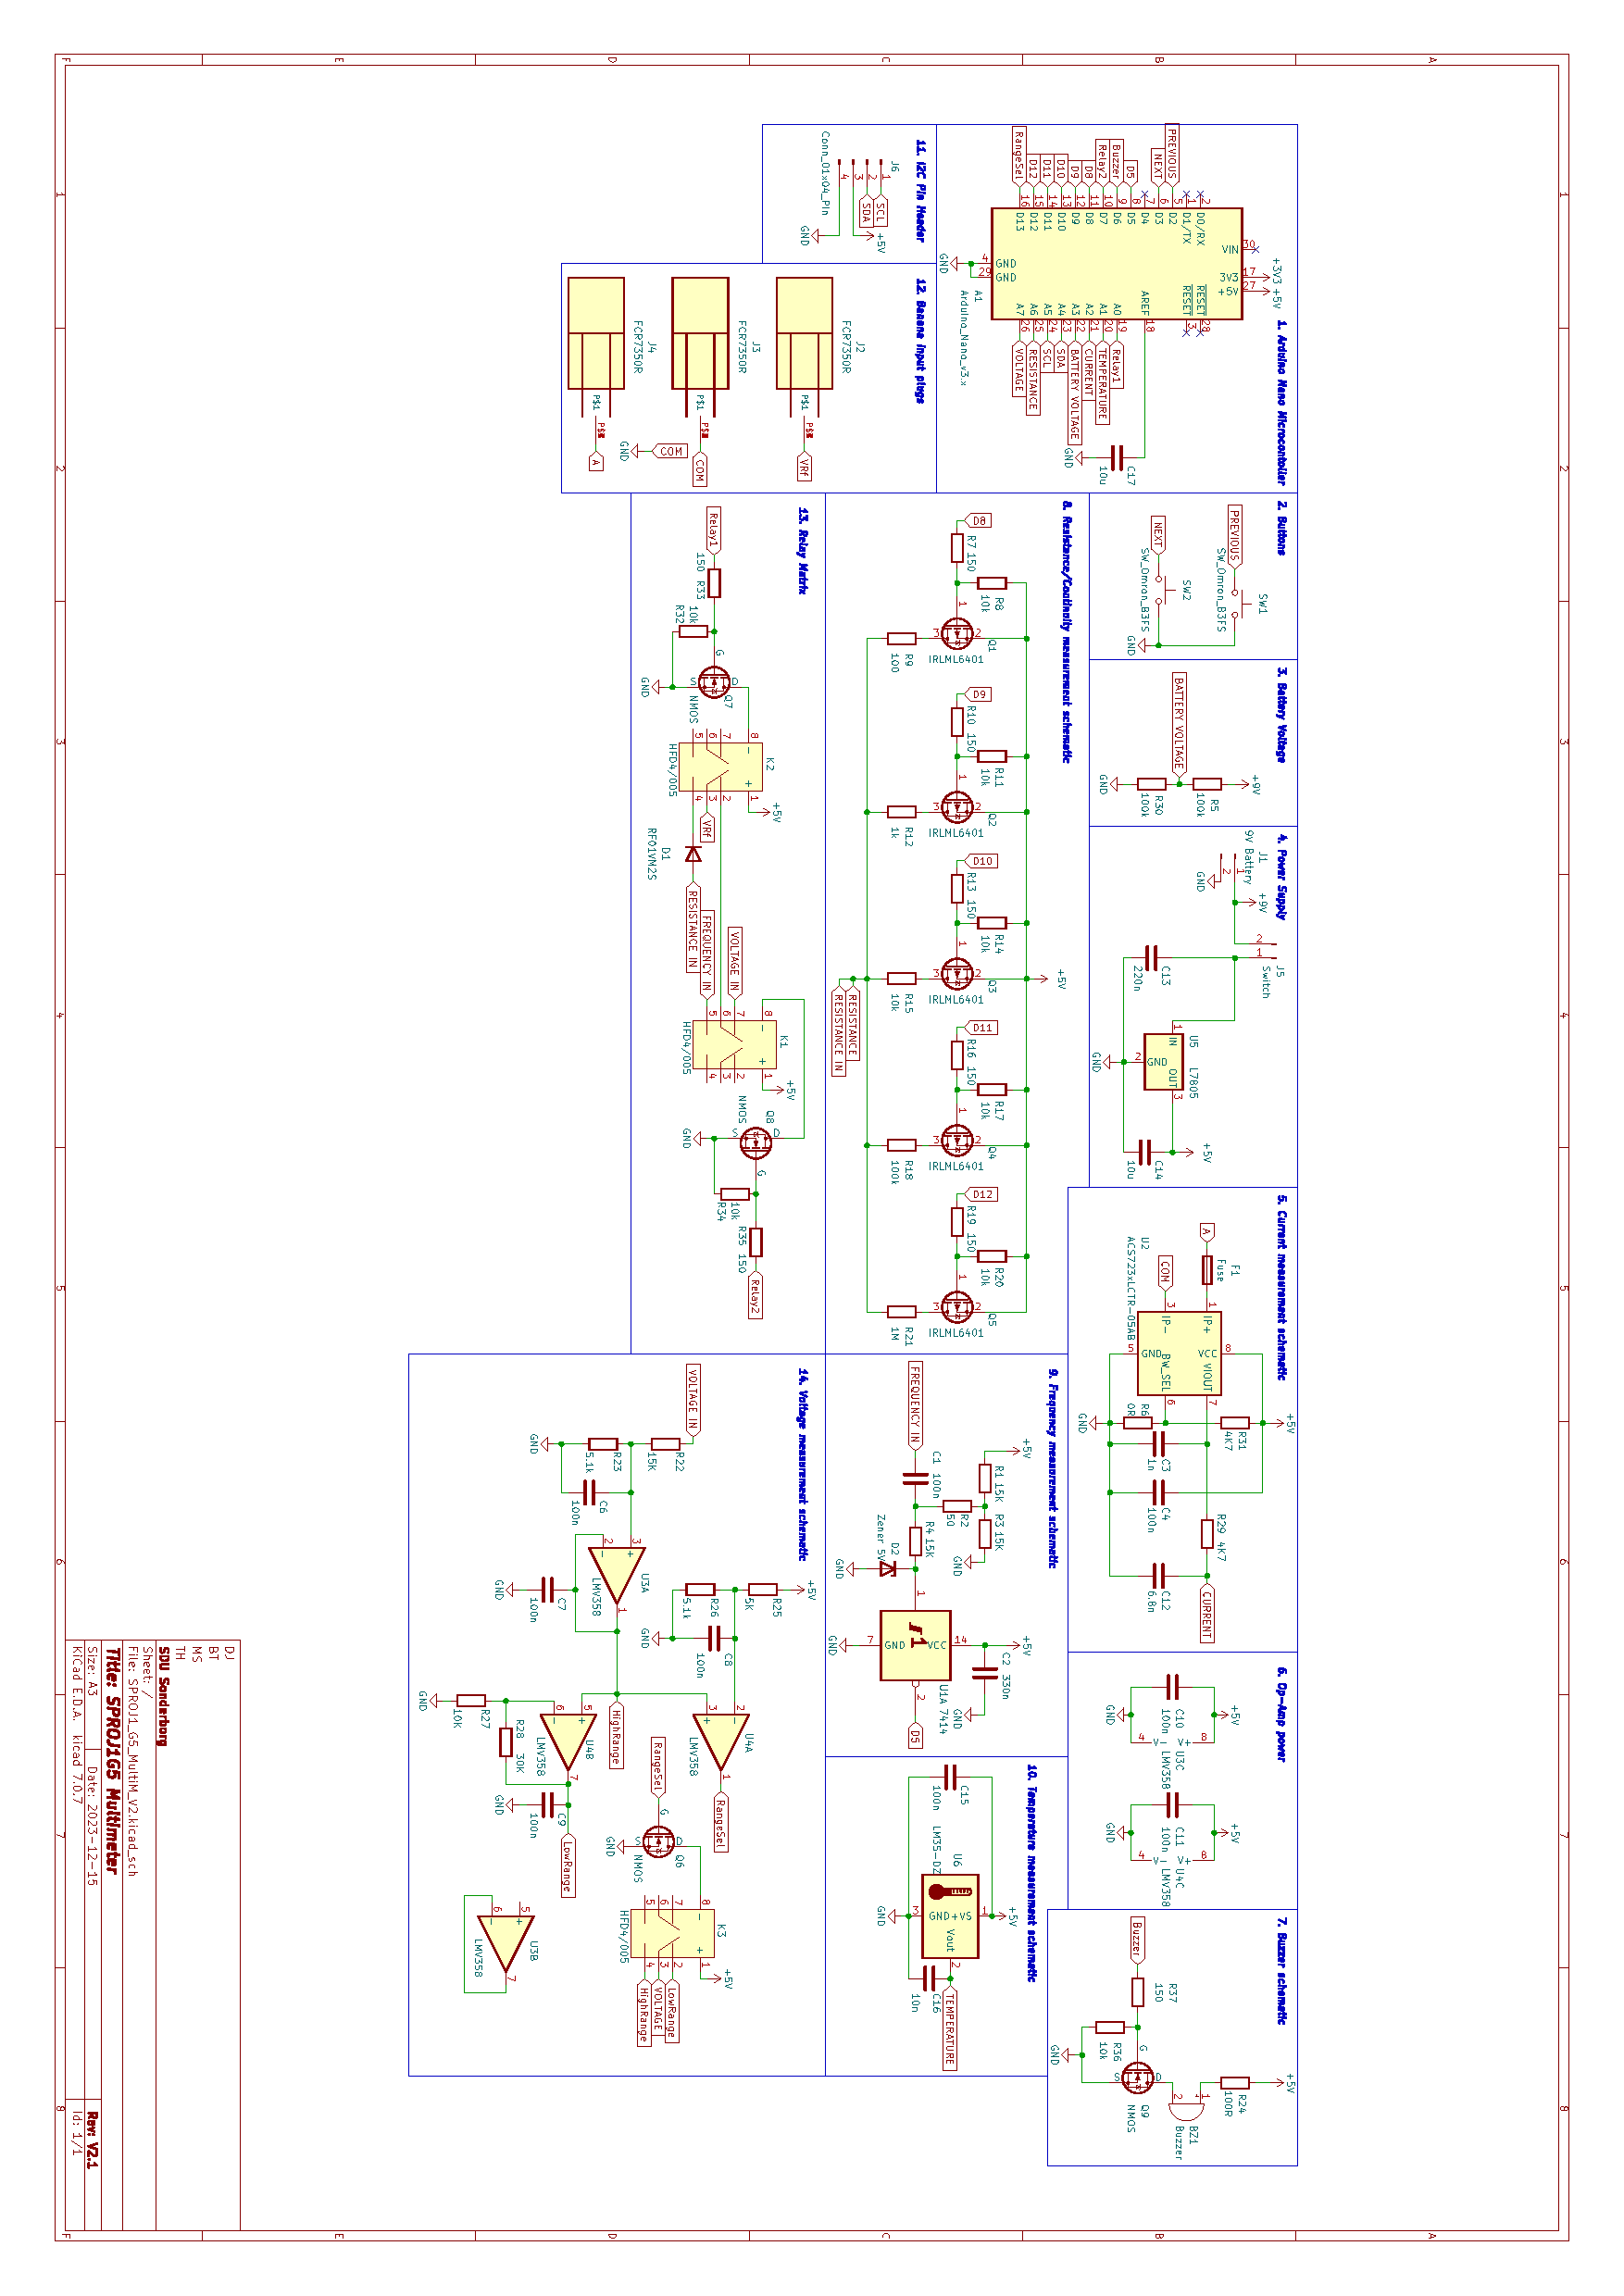
\includepdf[pages={1}]{Appendix/SPROJ1_G5_MultiM_V2.pdf}
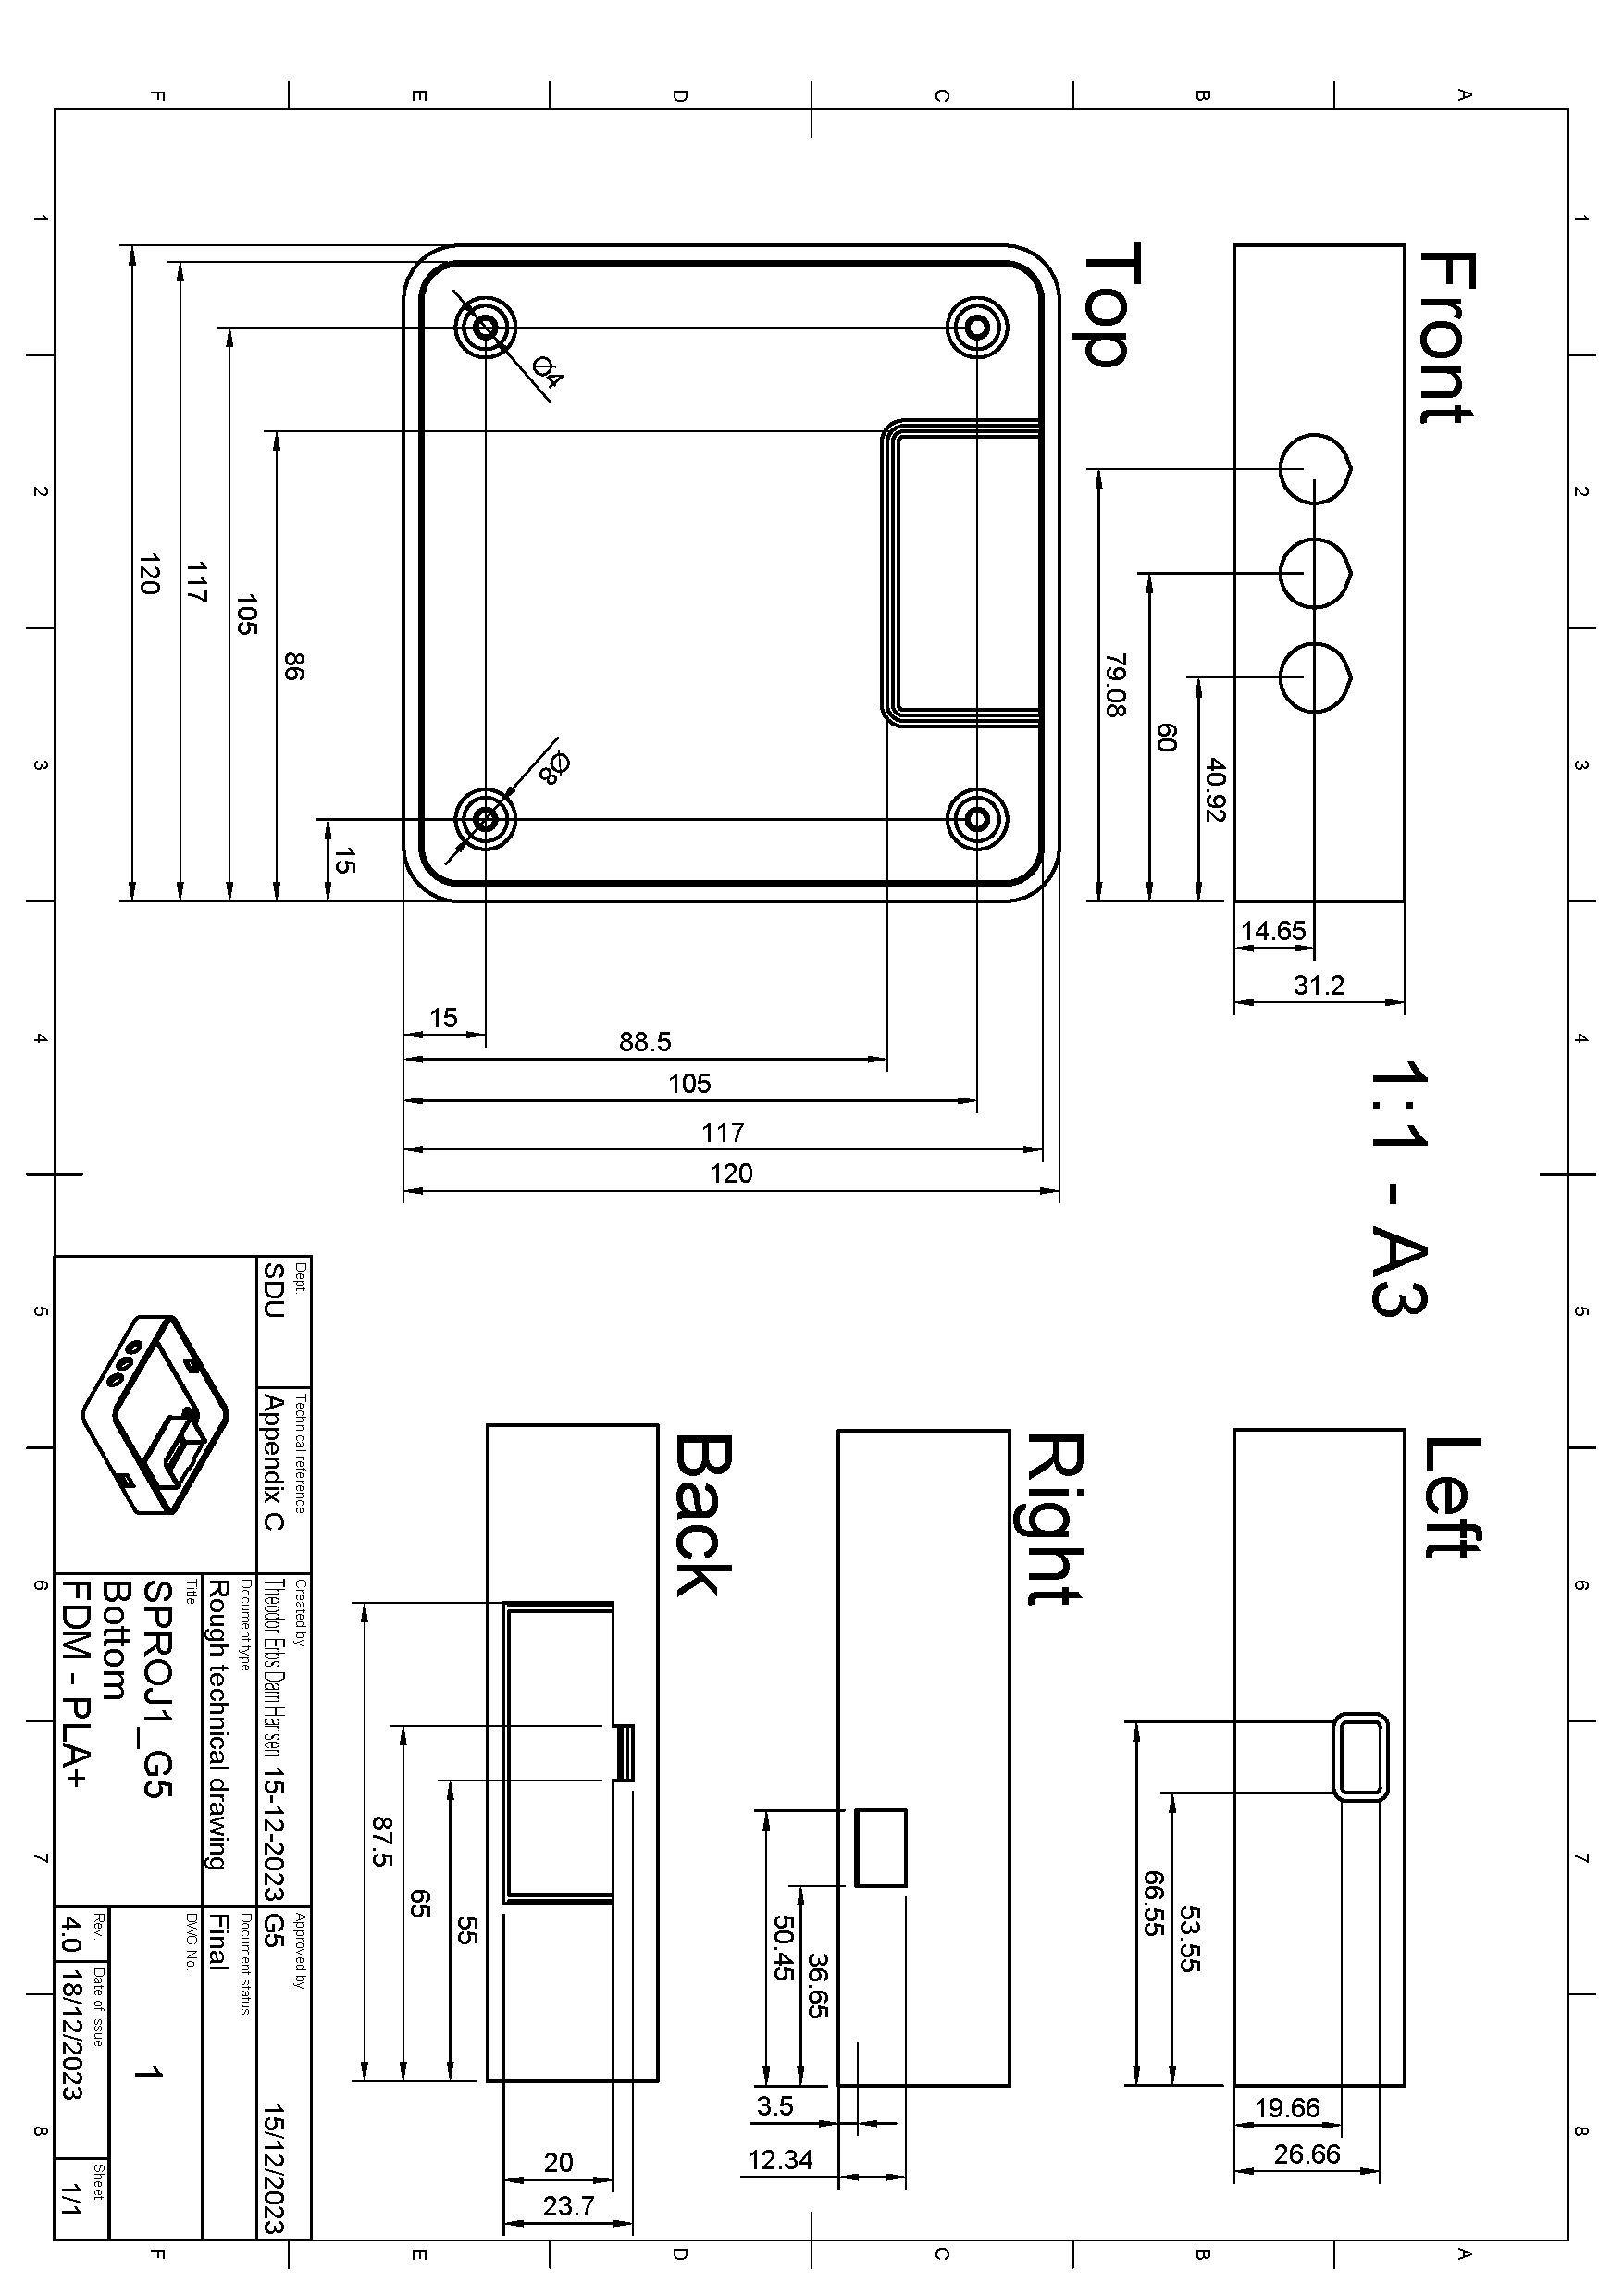
\includepdf[pages={1}]{Appendix/SPROJ1_SPIN02 Drawing v4.pdf}
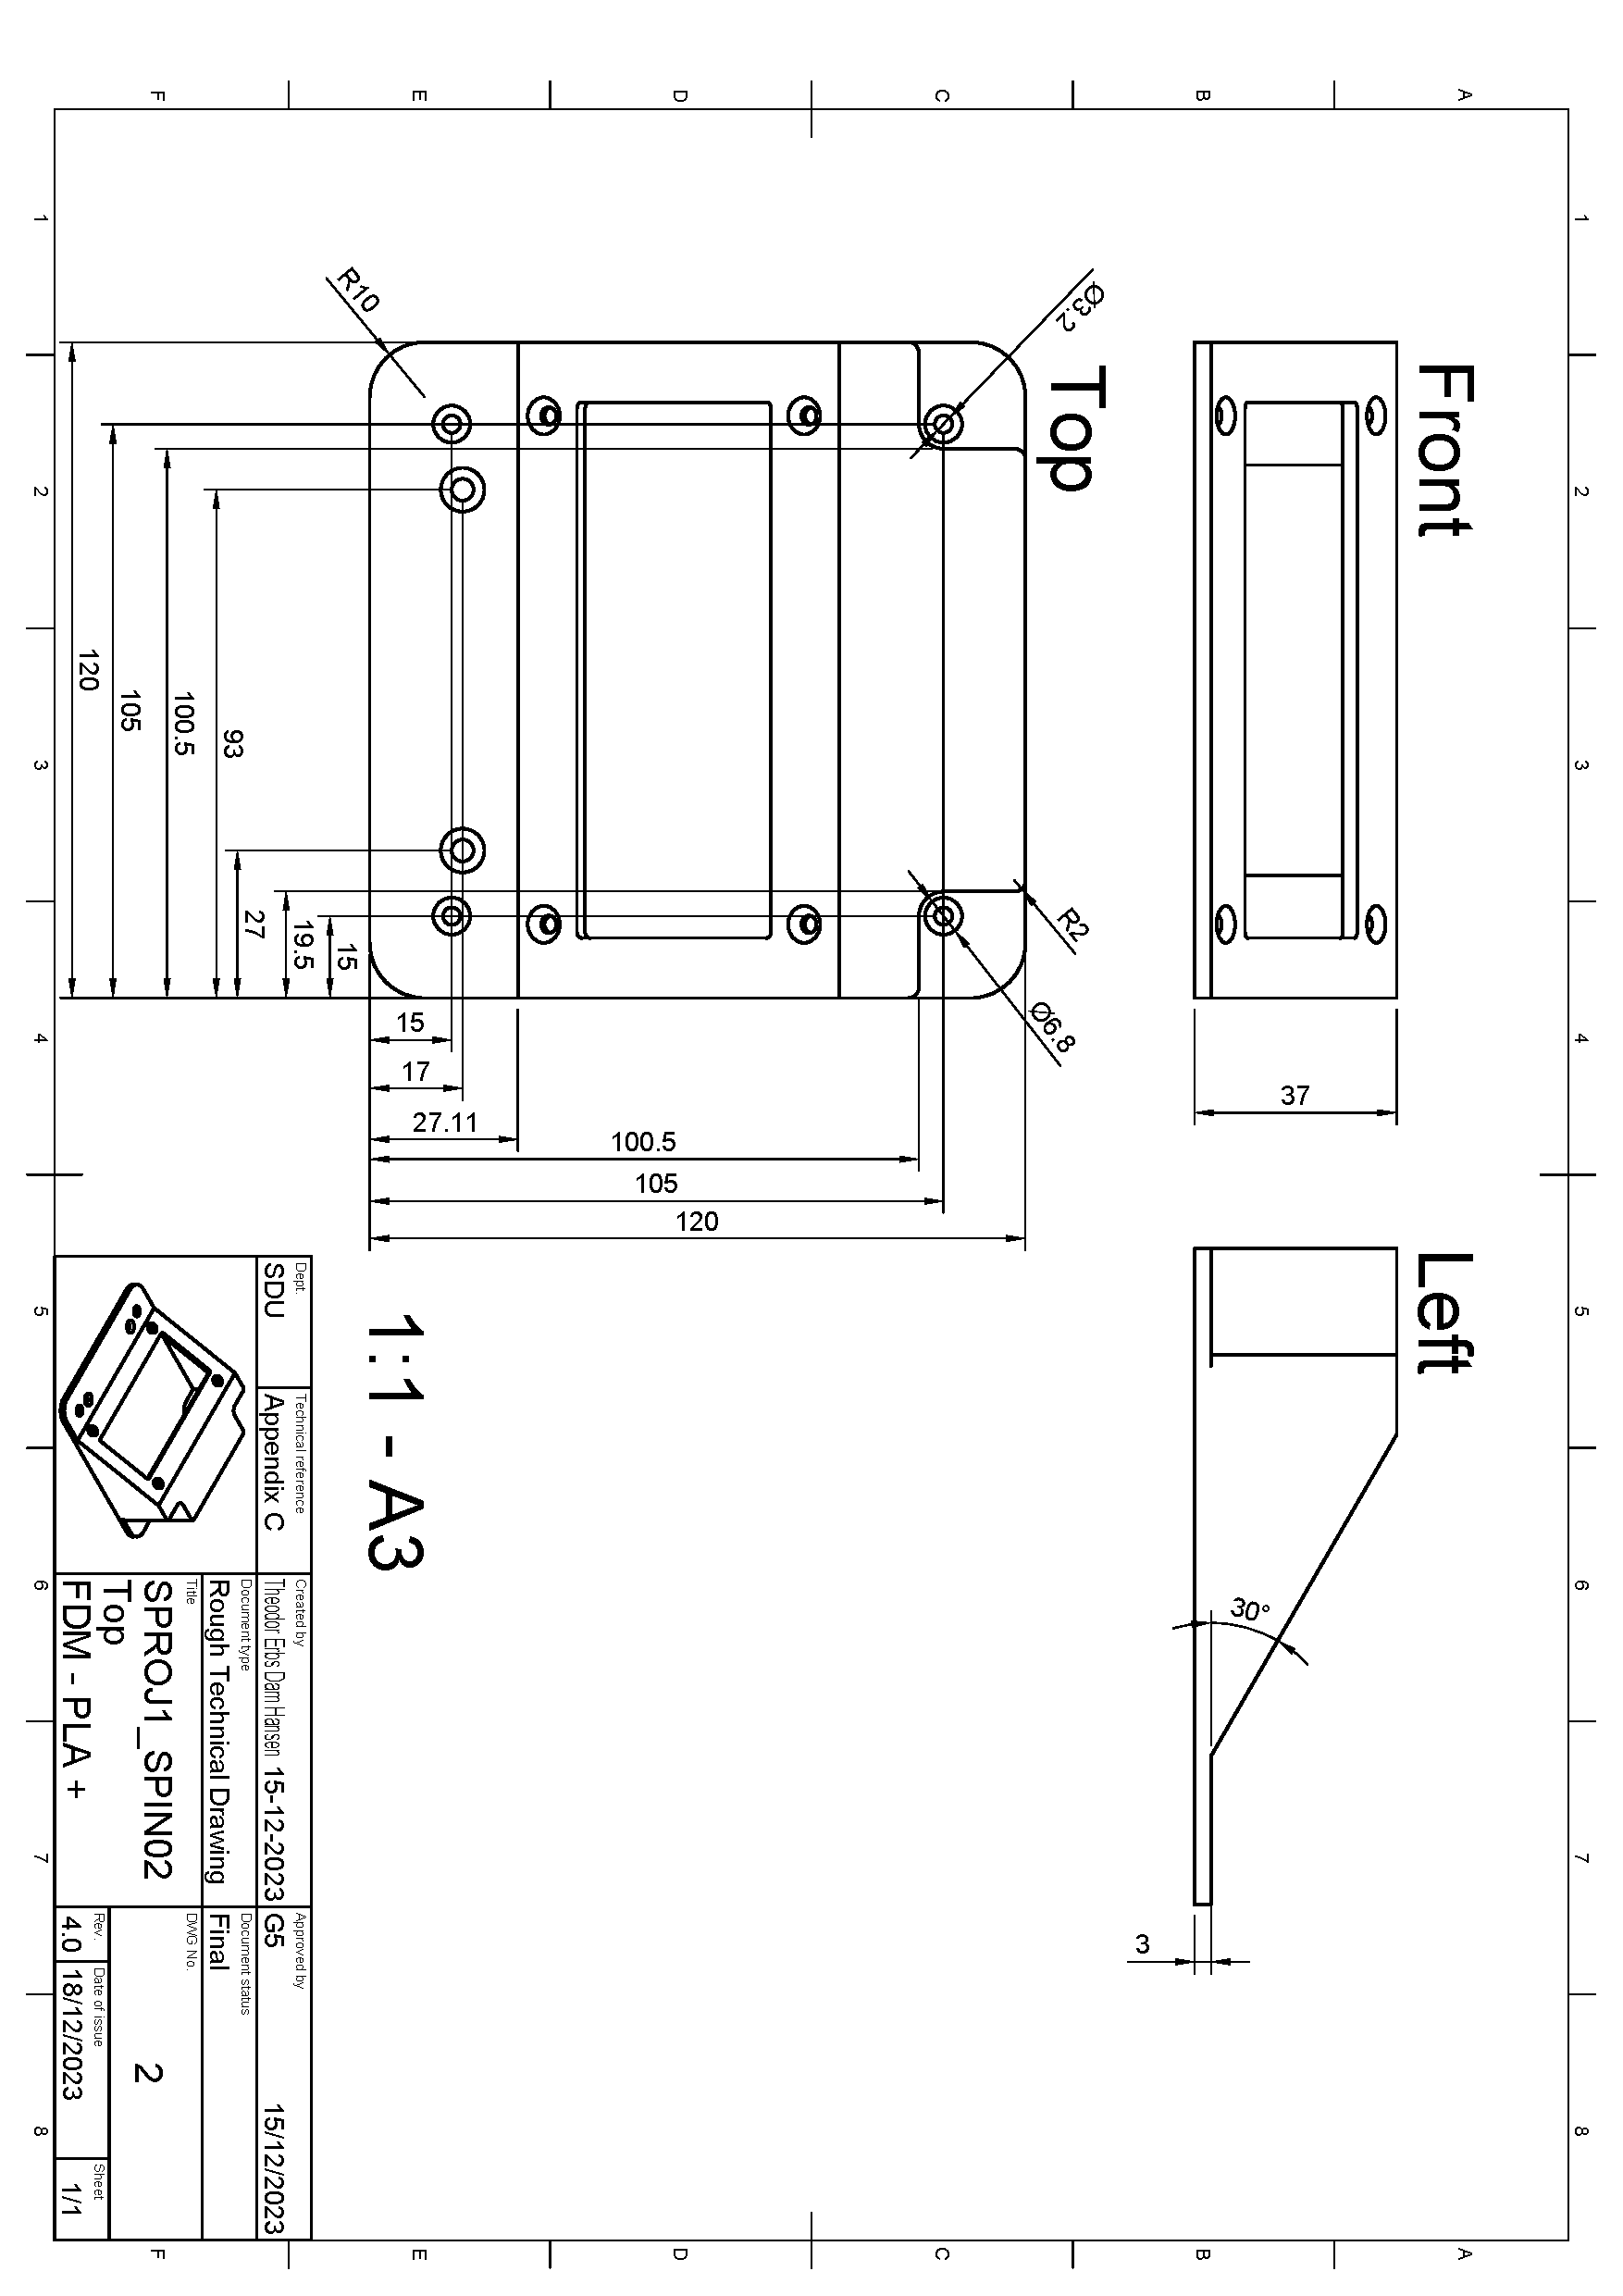
\includepdf[pages={1}]{Appendix/SPROJ1_SPIN02 Drawing top v6.pdf}
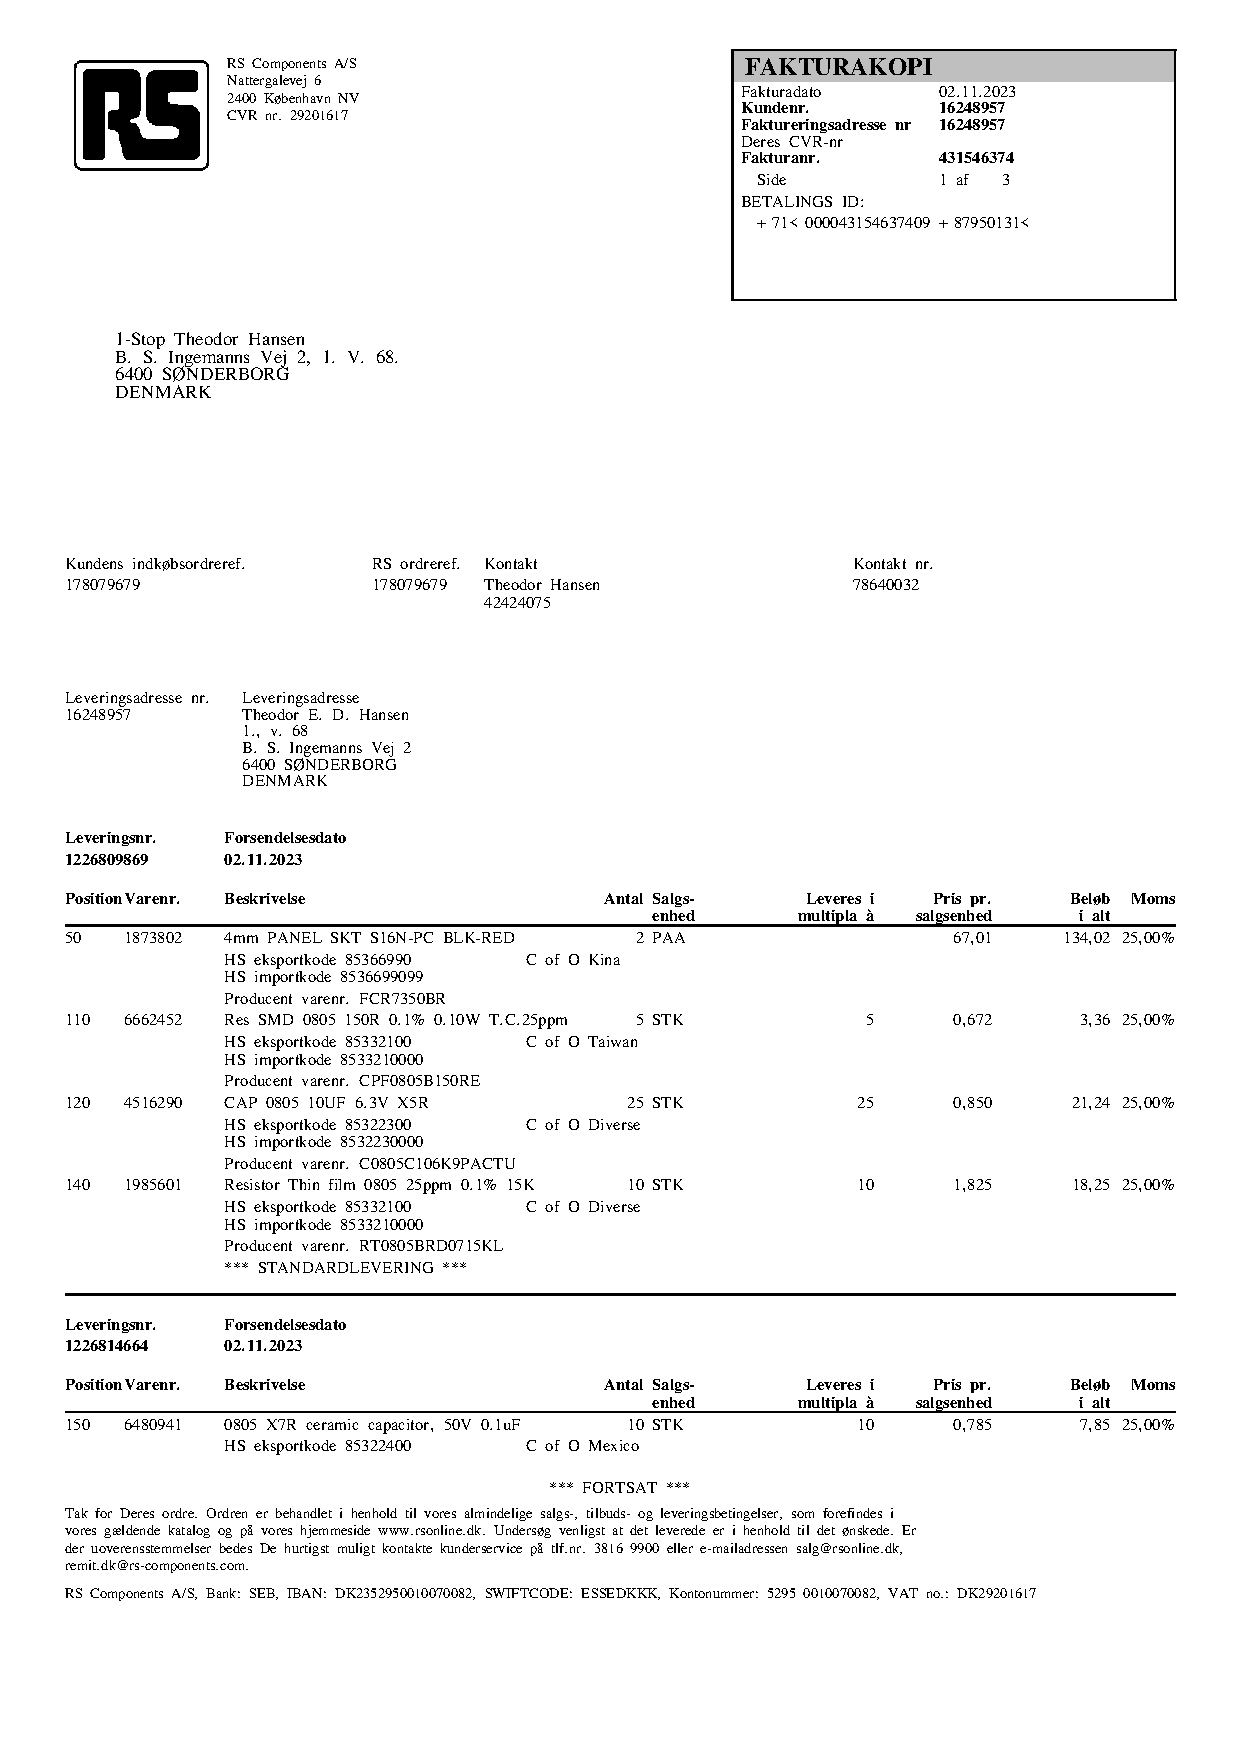
\includepdf[pages=-]{Appendix/BOM_RS.PDF}
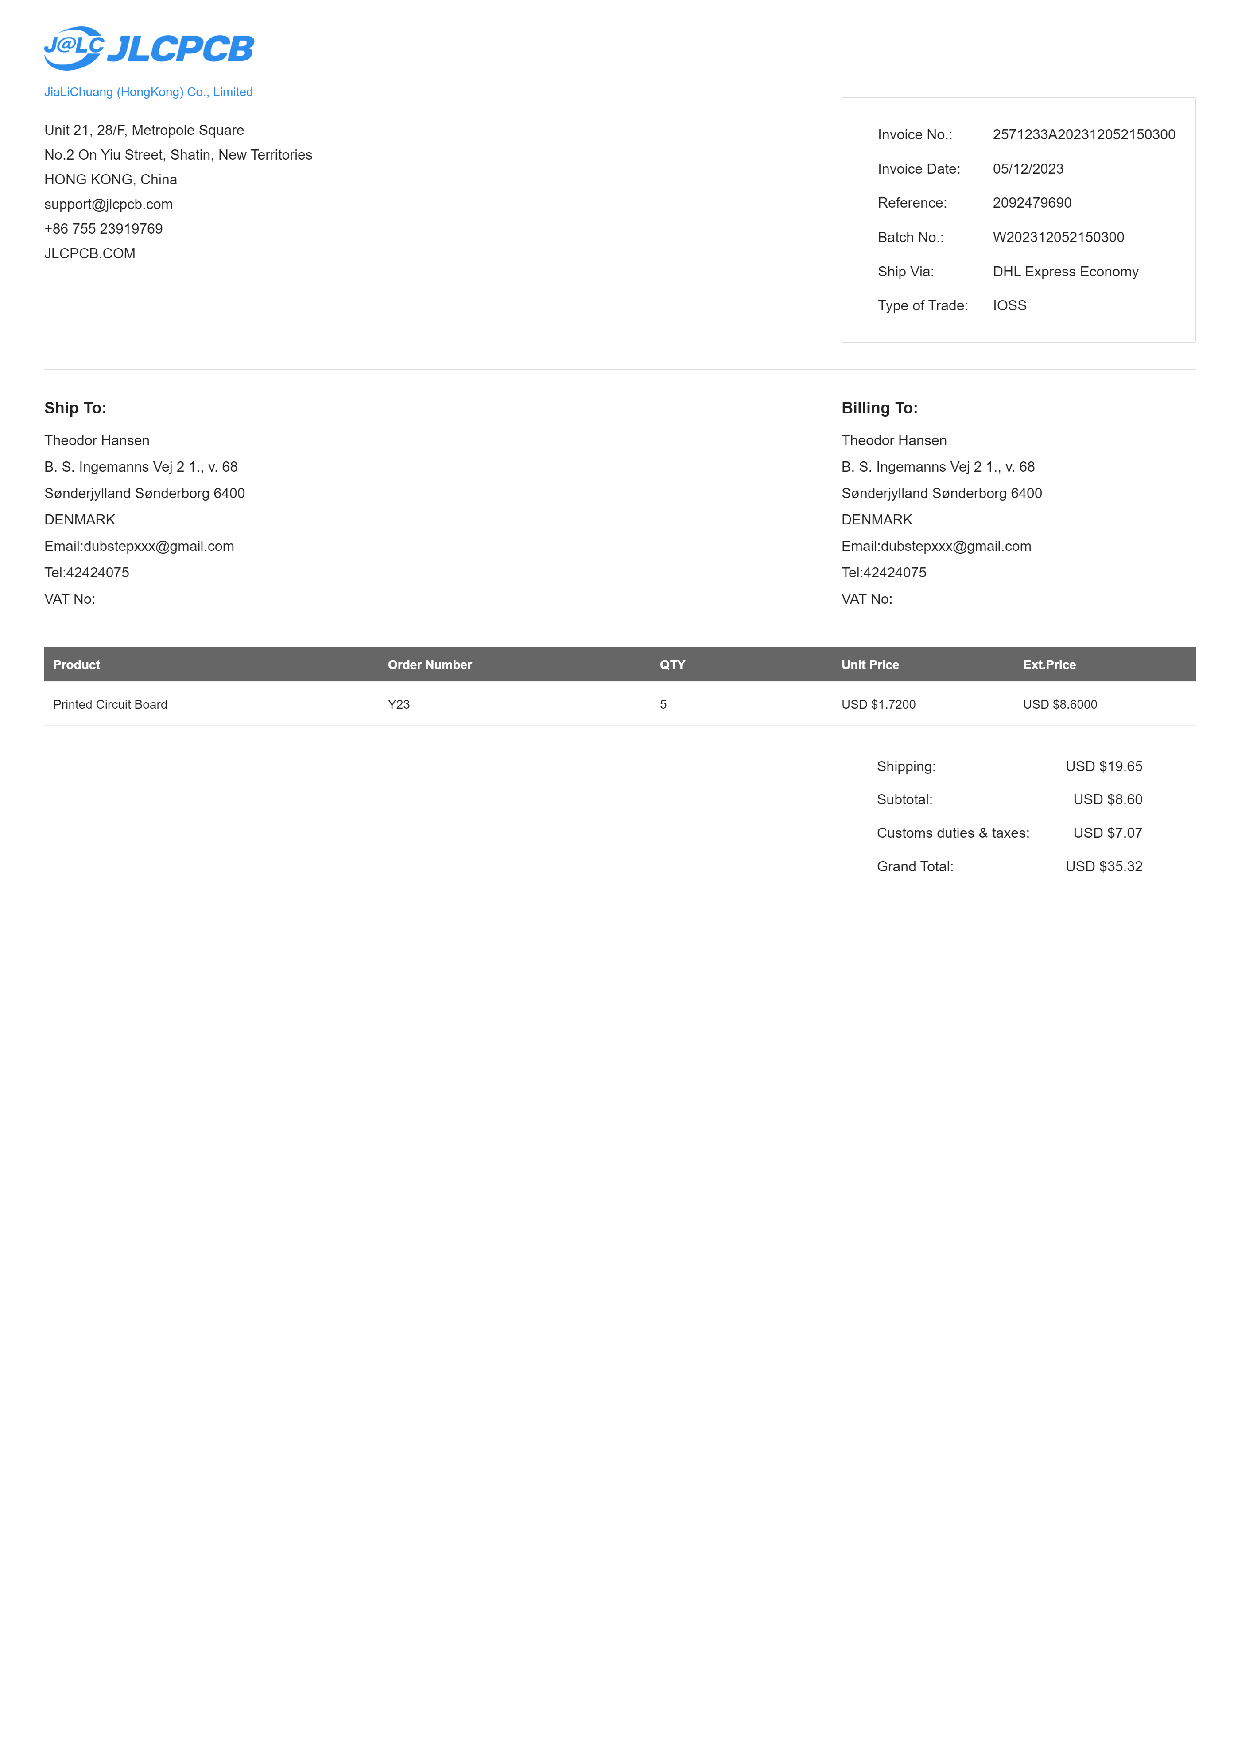
\includepdf[pages=-]{Appendix/JLCPCB_invoice.pdf}
\clearpage
\section{References}
\label{sec:references}

\begin{itemize}
    \item Arduino framework: \url{https://www.arduino.cc/reference/en/}
    \item LCD library: \url{https://github.com/johnrickman/LiquidCrystal_I2C}
    \item LM35 datasheet: \url{https://www.ti.com/lit/ds/symlink/lm35.pdf}
    \item LM35 library: \url{https://github.com/wilmouths/LM35}
    \item ACS723 datasheet: \url{https://www.allegromicro.com/~/media/files/datasheets/acs723-datasheet.ashx}
    \item LM7805 datasheet: \url{https://www.ti.com/lit/ds/symlink/lm7800.pdf}
    \item SN74HC14 datasheet: \url{https://www.ti.com/lit/ds/symlink/sn74hc14.pdf}
    \item LMV358 datasheet: \url{https://www.ti.com/lit/ds/symlink/lmv358a.pdf}
    \item Project firmware: \url{https://github.com/SPROJ1Group5/Project_Code}
    \item PCB design: \url{https://github.com/SPROJ1Group5/finalPCB}
    \item JLCPCB: \url{https://jlcpcb.com/}
    \item Monolithicpower: \url{http://tinyurl.com/3839sepf}
    \item Video showcase: \url{https://youtu.be/KzQqgtPINDI}
    \item TI Application brief: \url{http://tiny.cc/wmphvz}
\end{itemize}
\clearpage
\fancyhead{}
\begin{center}
NO LONGER PART OF THE OFFICIAL REPORT  

- 

this page is included as part of an agreement with Oliver Niebuhr.
\end{center}

\noindent This page highlights what each group member has contributed. For each section, the responsibility is delegated to a student, shown here. For shared responsibility and contribution, sections can be distributed to multiple students.
\vspace{5mm}

\noindent This document is written using \LaTeX\hspace{0.3mm} via the editor Overleaf. Its history function can document every change and addition done by assigned users.

\renewcommand{\arraystretch}{1.3}
\begin{center}
\begin{tabular}{ | m{2cm} | m{2cm}| m{2cm} | m{2cm} | } 
\hline
 \textbf{Theodor} & \textbf{Bence} & \textbf{Michał} & \textbf{Danial} \\ 
\hline
        \ref{sec:terminations} & \ref{sec:terminations} & \ref{sec:introduction} & \ref{sec:abstract}\\
        \ref{sec:method_current} & \ref{sec:method_frequency} & \ref{sec:method_voltage} & \\
        \ref{sec:method_resistance_idea} & \ref{sec:method_resistance_code} & \ref{sec:results_voltage} & \\
        \ref{sec:method_temperature} & \ref{sec:method_continuity} & \ref{sec:discussion_voltage} & \\
        \ref{sec:method_mechanical} & \ref{sec:method_switch_code} & \ref{sec:discussion_temperature} & \\
        \ref{sec:method_safety_relays} & \ref{sec:method_bat_indicator} & \ref{sec:conclusion} & \\
        \ref{sec:results_current} & \ref{sec:results_frequency} & \ref{sec:appendix} & \\
        \ref{sec:results_resistance} & \ref{sec:discussion_frequency} & \ref{sec:references} & \\
        \ref{sec:results_temperature} & \ref{sec:discussion_misc} &  & \\
        \ref{sec:discussion_current} & \ref{sec:appendix} &  & \\
        \ref{sec:discussion_resistance} & \ref{sec:references} &  & \\
        \ref{sec:discussion_mechanical} & & & \\
        \ref{sec:appendix} &  &  & \\
        \ref{sec:references} &  &  & \\
        \hline
\end{tabular}
\end{center}

\end{document}